% !TeX root = thesis.tex
%--------------------------------------------------------------------%
%
% Template TA LaTeX Teknik Informatika ITERA.
% Editor: Radhinka Bagaskara, Martin C.T. Manullang, I Wayan Wiprayoga Wisesa, Jose Alfredo Sitanggang (IF 2016), Ardoni Yeriko Rifana Gultom (IF 2021), Syabana Minggus Noviantosa (IF 2018), Rizki Alfaina (IF 2021)
% Version 2025.5
% TELAH DISESUAIKAN DENGAN FORMAT PERPUSTAKAAN ITERA MEI 2025 (UNESCO FORMAT)
%
% Berdasarkan "Templat LaTeX Tesis Informatika ITB" oleh Petra Barus & Peb Ruswono Aryan
% https://github.com/petrabarus/if-itb-latex
% Berdasarkan Panduan Tugas Akhir Teknik Informatika ITERA v1.3
% https://docs.google.com/document/d/1SYtSpRevbRvscXIJRAxuT41kJqqzsHyw/edit?usp=sharing&ouid=103935211052656359121&rtpof=true&sd=true
%
%--------------------------------------------------------------------%
%
% Berkas ini berisi struktur utama dokumen LaTeX yang akan dibuat.
%
%--------------------------------------------------------------------%

% Set jenis dokumen Tugas Akhir
\documentclass{report} % Untuk versi perpustakaan
\usepackage[paperwidth=155mm, % Setting layout kertas UNESCO (155 x 230 mm)
			paperheight=230mm,
			top=2cm,
			bottom=2cm,
			left=2cm,
			right=2cm,
			includefoot,
			heightrounded,
			bindingoffset=0.5cm]
			{geometry}

\input{config/config.sty} % Import konfigurasi laporan
\addbibresource{references.bib} % Import list Daftar Pustaka (gunakan addbibresource untuk biblatex)

\begin{document}

    %----------------------------------------------------------------%
    % Konfigurasi Informasi Tugas Akhir
    %----------------------------------------------------------------%

    % Judul Tugas Akhir, dalam Bahasa Indonesia
    \title{Implementasi Fine-Tuning OpenAI Whisper Base untuk Automatic Speech Recognition Bahasa Minangkabau}
    % Judul Tugas Akhir dalam Bahasa Inggris
    \titleEN{Implementation of OpenAI Whisper Base Fine-Tuning for Minangkabau Automatic Speech Recognition}
    % JUDUL AKAN DITULIS DALAM HURUF KAPITAL; Font size 16 pt; Bold; Tidak melebihi 4 baris

    % Informasi Mahasiswa
	\author{Fathan Andi Kartagama}		% Nama Mahasiswa
	\nim{122140055}				% NIM Mahasiswa

	%Informasi Dosen Pembimbing
	\dosbingA%
		{Martin Clinton Tosima Manullang, Ph.D.}%			% Nama Dosen Pembimbing 1
		{19930109 201903 1 017}	% NIP Dosen Pembimbing 1


	%Informasi Dosen Penguji
	\pengujiA%
		{I Wayan Wiprayoga Wisesa, S.Kom., M.Kom.}%				% Nama Dosen Penguji 1
		{NIP. 19890322 201903 1 009}	% NIP Dosen Penguji 1
	\pengujiB%
		{Prof. Sarwono Sutikno, Dr,Eng., CISA, CISSP, CISM, CSX-F, IIAP, CC}%				% Nama Dosen Penguji 2
		{NIP. 19591014 198503 1 003}	% NIP Dosen Penguji 2

	\sloppy % mencegah text overflow. (Jose)
    \pagenumbering{roman}
    \setcounter{page}{1} % Nomor halaman dimulai dengan "ii" di hal. Pengesahan

	%----------------------------------------------------------------%
	% Konten Laporan
	%----------------------------------------------------------------%
	\input{chapters/cover-hard} 	% Hardcover
	\input{chapters/approval} 		% Lembar Pengesahan
    %----------------------------------------------------------------%
    % Aktivasi twoside (agar ada margin gutter 0.5 cm) & nomor halaman selang-seling
    % mulai dari setelah Lembar Pengesahan (Ardoni)
    \clearpage
	\newgeometry{
		top=2cm,
		bottom=2cm,
		left=2cm,
		right=2cm,
		includefoot,
		heightrounded,
		bindingoffset=0.5cm,
		twoside % Agar halaman diset akan bolak-balik
	}
    \pagestyle{alternatingstyle}
    %----------------------------------------------------------------%
	\clearpage
\phantomsection% 
\addcontentsline{toc}{chapter}{HALAMAN PERNYATAAN ORISINALITAS}

\begin{center}
	\smallskip
	
%	\chapter*{\normalsize{Halaman Pernyataan Orisinalitas}}
	\large \bfseries \MakeUppercase{Halaman Pernyataan Orisinalitas} \linebreak
	
	\normalsize  \normalfont \justify \onehalfspacing{
		Saya yang bertanda tangan di bawah ini\\
		
		Menyatakan bahwa Tugas Akhir dengan judul : “{\thetitle}” adalah benar karya saya sendiri. Seluruh sumber baik yang dikutip maupun dirujuk dalam penulisan tugas akhir ini telah saya cantumkan secara benar sesuai dengan kaidah penulisan ilmiah.\\
		
		Apabila di kemudian hari ditemukan adanya unsur plagiarisme dalam karya ini, maka saya bersedia menerima sanksi sesuai ketentuan yang berlaku di institusi saya.\\
		
		Demikian pernyataan ini saya buat dengan sesungguhnya.
		}
	\vspace{3cm}
	
	\centering 
	Lampung Selatan, \todayIndo\\
	\vspace{2cm}
	\theauthor\\
	NIM. \printnim
\end{center}
\clearpage
 		% Halaman Pernyataan Orisinalitas
	\input{chapters/publication} 	% Halaman Persetujuan Publikasi
	\clearpage
\phantomsection% 
\addcontentsline{toc}{chapter}{KATA PENGANTAR}
%\thispagestyle{fancy}

\begin{justifying}
	\large \bfseries \centering \MakeUppercase{Kata Pengantar}\linebreak
	
	\normalsize \normalfont \justifying
	Puji syukur ke hadirat Tuhan Yang Maha Esa atas segala rahmat dan karunia-Nya, sehingga penulis dapat menyelesaikan tugas akhir ini dengan baik.
    
    Penyusunan tugas akhir ini tidak terlepas dari bimbingan dan dukungan berbagai pihak. Oleh karena itu, penulis mengucapkan terima kasih yang sebesar-besarnya kepada:
    \begin{enumerate}
        \item Bapak Martin Clinton Tosima Manullang, Ph.D., selaku Dosen Pembimbing yang telah meluangkan waktu dan tenaga untuk mengarahkan penulis hingga tugas akhir ini selesai.
        \item Bapak I Wayan Wiprayoga Wisesa, S.Kom., M.Kom., Radhinka Bagaskara, S.Si.Kom., M.Si., M.Sc., dan Prof. Sarwono Sutikno, Dr, Eng., selaku Dosen Penguji yang telah memberikan masukan, kritik, serta saran konstruktifnya.
        \item Ibu tercinta yang senantiasa memberikan doa yang tak terputus, kasih sayang yang tulus, serta motivasi yang tiada henti kepada penulis dalam setiap langkah.
        \item Kedua kakak dan kedua abang ipar atas dorongan semangat serta dukungannya selama proses penulisan.
        \item Bapak Cahya Wirawan atas penyediaan dan pemeliharaan dataset LibriVox Indonesia di HuggingFace yang sangat membantu penelitian ini.
        \item Seluruh pihak yang tidak dapat disebutkan satu per satu atas segala bantuan dan dukungannya.
    \end{enumerate} 
    
    Penulis menyadari bahwa tugas akhir ini masih jauh dari sempurna. Semoga karya ini dapat memberikan manfaat dan wawasan yang berguna bagi para pembaca.
	
\end{justifying}
\clearpage 		% Kata Pengantar
	\clearpage
\phantomsection% 
\addcontentsline{toc}{chapter}{RINGKASAN}
\thispagestyle{fancy}

\begin{center}
	\large \bfseries \MakeUppercase{Ringkasan}\\
	\normalsize \normalfont {\thetitle}\\
	\normalsize \normalfont {\theauthor}\\
	\bigskip
\end{center}

	\normalsize \normalfont \justifying \singlespacing
	Perkembangan teknologi \textit{Automatic Speech Recognition} (ASR) saat ini telah mencapai kemajuan yang signifikan. Namun, mayoritas sistem ASR yang ada masih berfokus pada bahasa mayor dan kurang mendukung bahasa daerah yang termasuk dalam kategori bahasa dengan sumber daya rendah (\textit{low-resource language}), seperti bahasa Minangkabau. Ketiadaan dataset berskala besar yang teranotasi dengan baik dan kompleksitas variasi dialek menjadikan pemodelan ASR untuk bahasa Minangkabau sebagai sebuah tantangan komputasi. Berdasarkan permasalahan tersebut, penelitian ini merumuskan masalah mengenai bagaimana mengimplementasikan dan mengevaluasi metode pembelajaran agar akurasi sistem ASR untuk bahasa Minangkabau dapat ditingkatkan. Tujuan dari penelitian ini adalah untuk mengadaptasi model bahasa universal ke dalam bahasa daerah secara efisien serta mengukur peningkatannya.

	Metodologi penelitian yang dilakukan berpusat pada proses \textit{fine-tuning} model \textit{pre-trained} OpenAI Whisper varian Base. Mengingat bahasa Minangkabau merupakan bahasa \textit{low-resource} dengan ketidakseimbangan frekuensi kemunculan fonem, penelitian ini menerapkan teknik \textit{Parameter-Efficient Fine-Tuning} (PEFT) melalui arsitektur \textit{Low-Rank Adaptation} (LoRA) untuk meminimalisasi beban komputasi selama pelatihan. Selain itu, digunakan pula optimasi berbasis \textit{Weighted Cross-Entropy Loss} guna menangani distribusi data yang tidak seimbang (\textit{data imbalance}) pada hierarki karakter, sehingga tebakan model tidak bias pada karakter yang umum saja. Evaluasi diukur secara kuantitatif dengan membandingkan nilai \textit{Word Error Rate} (WER) dan \textit{Character Error Rate} (CER) antara model \textit{zero-shot} bawaan model dasar dengan model hasil adaptasi.

	Hasil dan analisis observasi membuktikan bahwa proses \textit{fine-tuning} berhasil menekan persentase kesalahan prediksi secara substansial. Model Whisper yang telah di-\textit{fine-tuning} dengan modifikasi bobot mampu mengenali dan mentranskripsikan tuturan Minangkabau lebih akurat ketimbang generasi bawaannya. Di tingkat fonem, penerapan \textit{Weighted Cross-Entropy} membantu meluruskan kekeliruan pemetaan fonetik, meskipun sistem masih mendapati residu kesalahan ketika dihadapkan dengan penutur dari kawasan berdilek kental, seperti dari daerah Agam atau Lima Puluh Kota, yang memiliki serapan kata berbeda.

	Kesimpulan dari penelitian ini menegaskan bahwa pendekatan \textit{fine-tuning} menggunakan LoRA dipadukan dengan \textit{Weighted Cross-Entropy} pada OpenAI Whisper merupakan solusi yang sangat efektif bagi masalah ASR pada bahasa lokal. Perpaduan ini membuahkan performansi transkripsi yang jitu murni dengan mempertahankan efisiensi waktu komputasi. Sebagai saran untuk pengembangan selanjutnya, pengumpulan korpus data wicara yang lebih masif direkomendasikan sebagai prioritas utama. Perbanyakan data dapat dilakukan melintasi beragam kabupaten melalui metode \textit{crowdsourcing} penutur asli maupun ekstraksi arsip dari media siaran lokal agar model dapat terus berekspansi menangkap luasnya diksi verbal Minangkabau yang sesungguhnya.

\vfill
\clearpage 		% Ringkasan
	\clearpage
\phantomsection% 
\addcontentsline{toc}{chapter}{ABSTRAK}
\thispagestyle{fancy}

\begin{center}
	\large \bfseries \MakeUppercase{Abstrak}\\
%	\normalsize \normalfont {\thetitle}\\
%	\normalsize \normalfont {\theauthor}\\
	\bigskip
	
	\normalsize \normalfont \justifying \singlespacing
	Teknologi pengenalan wicara atau \textit{Automatic Speech Recognition} (ASR) saat ini mayoritas terpusat pada bahasa dengan sumber daya besar (\textit{high-resource}), sementara bahasa daerah seperti Minangkabau yang berstatus \textit{extremely low-resource} (1,3 jam data latih) belum terfasilitasi dengan baik. Hal ini mengakibatkan rendahnya akurasi sistem ASR generik akibat kompleksitas ragam dialek lokal. Penelitian ini bertujuan untuk meningkatkan akurasi sistem ASR bahasa Minangkabau melalui implementasi \textit{fine-tuning} pada model \textit{pre-trained} OpenAI Whisper Base. Metodologi difokuskan pada teknik \textit{Parameter-Efficient Fine-Tuning} (PEFT) menggunakan \textit{Low-Rank Adaptation} (LoRA) untuk meminimalisasi beban komputasi, serta dibandingkan dengan strategi \textit{Freeze Encoder}. Selain itu, fungsi \textit{Weighted Cross-Entropy} (WCE) dengan pemisahan temporal diperkenalkan untuk menangani ketidakseimbangan sebaran fonem tanpa membocorkan data validasi. Performa model dievaluasi menggunakan skema 5-\textit{Fold Cross-Validation} dengan metrik \textit{Word Error Rate} (WER) dan \textit{Character Error Rate} (CER). Hasil pengujian mengonfirmasi bahwa LoRA secara konsisten mengungguli \textit{Freeze Encoder}, mencapai rata-rata WER 15,67\% dan CER 3,32\% dengan hanya melatih 2,93\% parameter model. Kesimpulannya, kombinasi LoRA dan pembobotan WCE terbukti efektif dan efisien dalam mentranskripsi bahasa Minangkabau, meskipun masih menyisakan sedikit tantangan pada tuturan fonetik logat spesifik. Di masa depan, perluasan korpus wicara melalui skema \textit{crowdsourcing} menjadi rekomendasi untuk penelitian lanjutan.\par

    \vspace{20pt}
	\raggedright \textbf{Kata Kunci}: Pengenalan Wicara, OpenAI Whisper, Minangkabau, \textit{Fine-Tuning}, LoRA
    
	\vfill
	
\end{center}
\clearpage 	% Abstrak (Indonesia)
	\clearpage
\phantomsection% 
\addcontentsline{toc}{chapter}{ABSTRACT}
\thispagestyle{fancy}

\begin{center}
	\large \bfseries \MakeUppercase{Abstract}\\
	\normalsize \normalfont {\thetitleEN}\\
	\normalsize \normalfont {\theauthor}\\
	\bigskip
	
	\normalsize \normalfont \justifying \singlespacing
    Automatic Speech Recognition (ASR) technology is currently predominantly centered on high-resource languages, while regional languages such as Minangkabau, which are extremely low-resource (1.3 hours of training data), remain inadequately facilitated. This results in the low accuracy of generic ASR systems due to the complexity of local dialect variations. This study aims to improve the accuracy of Minangkabau language ASR systems through the implementation of fine-tuning on the pre-trained OpenAI Whisper Base model. The methodology focuses on the Parameter-Efficient Fine-Tuning (PEFT) technique using Low-Rank Adaptation (LoRA) to minimize computational load, and is compared against the Freeze Encoder strategy. Furthermore, a Weighted Cross-Entropy (WCE) function with temporal separation is introduced to address the imbalance of phoneme distribution without leaking validation data. Model performance is evaluated using a 5-Fold Cross-Validation scheme with Word Error Rate (WER) and Character Error Rate (CER) metrics. The experimental results confirm that LoRA consistently outperforms the Freeze Encoder, achieving an average WER of 15.67\% and CER of 3.32\% while only training 2.93\% of the model parameters. In conclusion, the combination of LoRA and WCE weighting proves to be effective and efficient in transcribing the Minangkabau language, although minor challenges remain with specific dialectal phonetic utterances. In the future, expanding the speech corpus through a crowdsourcing scheme is recommended for further research.\par

    \vspace{20pt}
    \raggedright \textbf{Keywords}: Speech Recognition, OpenAI Whisper, Minangkabau, Fine-Tuning, LoRA
    
	\vfill
	
\end{center}
\clearpage 	% Abstrak (Inggris)
    %----------------------------------------------------------------%
    % Halaman Daftar
    %----------------------------------------------------------------%
	% Daftar Isi
	\phantomsection%
	\addcontentsline{toc}{chapter}{DAFTAR ISI}
	\tableofcontents
	% Daftar tabel
	\phantomsection%
	\addcontentsline{toc}{chapter}{DAFTAR TABEL}
	\listoftables
	% Daftar gambar
	\phantomsection%
	\addcontentsline{toc}{chapter}{DAFTAR GAMBAR} % TODO: No halaman ga selang-seling di Daftar? (RDB)
	\listoffigures
	% Daftar rumus
	% \pagestyle{daftarrumusstyle}
	\phantomsection%
	\addcontentsline{toc}{chapter}{DAFTAR RUMUS}
	\listofmyequations
	% \thispagestyle{daftarrumusstyle}
	% \pagebreak
	%    \input{chapters/symbols}
	% Daftar kode
	\phantomsection%
	\addcontentsline{toc}{chapter}{DAFTAR KODE}
	\lstlistoflistings
	\pagebreak
    %----------------------------------------------------------------%
    % Konfigurasi Bab
    %----------------------------------------------------------------%
    \renewcommand{\chaptername}{BAB}
    % Bab: Arabic
    \renewcommand{\thechapter}{\Roman{chapter}}
    % Sub-bab: Roman
    \renewcommand\thesection{\arabic{chapter}.\arabic{section}}
    % Setting supaya nomor halaman pertama dengan "chapter"
    % berada di tengah bawah, tapi selanjut2nya di kanan atas
    \fancypagestyle{plain}{%
    	\fancyhf{}%
    	\renewcommand{\headrulewidth}{0pt}
    	\fancyhead[]{}
    	\fancyfoot[C]{\thepage}
    }
    % Reset penomoran halaman menjadi 1
    \setcounter{page}{1}
    \pagenumbering{arabic}
    \justifying
    % Mulai selang-seling halaman
    \forceoddpage
    \cleardoublepage
    \pagestyle{alternatingstyle}
    %----------------------------------------------------------------%
    % Daftar Bab
    % Untuk menambahkan daftar bab, buat berkas bab misalnya `chapter-6` di direktori `chapters`, dan masukkan ke sini.
    %----------------------------------------------------------------%
    \newpage
\chapter{PENDAHULUAN} \label{Bab I}

\section{Latar Belakang} \label{I.Latar Belakang}
Dalam beberapa dekade terakhir, kemajuan dalam pemrosesan suara dan pengenalan ucapan (\textit{Automatic Speech Recognition} / ASR) telah menjadi salah satu bidang riset yang sangat penting, terutama karena potensinya besar di banyak aspek kehidupan manusia, misalnya asisten suara (\textit{Siri, Google Assistant}), sistem transkripsi otomatis, aksesibilitas bagi penyandang disabilitas, layanan publik, pendidikan, serta interaksi manusia-komputer. Model-model berbasis pembelajaran mendalam (\textit{deep learning}) yang menggunakan arsitektur \textit{Transformer}, atau model "\textit{end-to-end}", semakin banyak digunakan untuk menggantikan pendekatan tradisional seperti \textit{Hidden Markov Model dan Gaussian Mixture Model}. \par

Namun, performa ASR sangat bergantung pada ketersediaan data berbicara (\textit{speech}) dan transkripsi yang berkualitas dan representatif dari bahasa atau dialek target. Untuk bahasa mayor seperti Inggris, Mandarin, Spanyol, data sangat melimpah; sementara untuk bahasa lokal atau dialek (termasuk bahasa daerah di Indonesia) data seringkali sangat terbatas (\textit{low-resource}). Model yang telah dilatih pada data multibahasa besar seperti Whisper kadang masih kurang optimal ketika menghadapi dialek atau bahasa yang kurang terwakili dalam data latihannya. \par

OpenAI memperkenalkan model Whisper sebagai model \textit{speech-to-text} multibahasa dengan pelatihan lemah-supervisi skala besar (\textit{Large-Scale Weak Supervision}) (sekitar 680.000 jam data audio transkrip) untuk generalisasi ke berbagai kondisi dan bahasa \cite{radford2023whisper}. Meskipun demikian, model dasar ("\textit{base Whisper}") seringkali tidak menghasilkan akurasi memadai ketika dihadapkan pada bahasa atau dialek yang sangat spesifik atau dengan variasi fonetik tinggi yang belum banyak direpresentasikan. Oleh karena itu, teknik \textit{fine-tuning} terhadap model dasar menjadi sangat penting agar model "teradaptasi" ke karakteristik bahasa lokal tersebut. \par

Teknik \textit{fine-tuning} Whisper telah dieksplorasi dalam sejumlah studi, terutama untuk bahasa \textit{low-resource}. Misalnya, penelitian \textit{Exploration of Whisper fine-tuning strategies for low-resource ASR} menunjukkan bahwa berbagai strategi \textit{fine-tuning} dapat secara signifikan meningkatkan performa pengenalan suara untuk bahasa-bahasa dengan data terbatas \cite{liu2024exploration}. Ada pula penelitian "\textit{Fine-tuning Whisper on Low-Resource Languages for Real-World Applications}" yang memperkenalkan metode transformasi dataset kalimat-ke-audio panjang untuk menjaga kemampuan segmentasi dan bagus bagi aplikasi nyata \cite{timmel2024finetune}. \par

Studi lain mengusulkan metode \textit{fine-tuning} efisien, seperti \textit{LoRA-Whisper}, yang bertujuan agar adaptasi ke bahasa baru bisa dilakukan tanpa menurunkan performa bahasa lain dan dengan \textit{overhead} parameter yang lebih kecil \cite{song2024lorawhisper}. Juga ada penelitian \textit{Multistage Fine-tuning Strategies for Automatic Speech Recognition in Low-resource Languages} yang menggunakan strategi \textit{multistage} (bertahap) untuk mengadaptasi model melalui bahasa yang punya kemiripan linguistik \cite{pillai2024multistage}. \par

Begitu juga, studi aplikasi domain khusus (misalnya dalam konteks medis) menekankan bahwa \textit{fine-tuning} model Whisper pada domain spesifik (dengan kosakata dan pola suara khusus) mampu meningkatkan akurasi dibandingkan model standar \cite{banerjee2024unitedmedasr}. Dengan demikian, adaptasi model ASR (melalui \textit{fine-tuning}) telah menjadi pendekatan penting untuk menjembatani kesenjangan antara model umum dan kebutuhan lokal atau domain khusus. \par

Di Indonesia, keragaman bahasa dan dialek sangat tinggi, dan banyak komunitas menggunakan bahasa daerah dalam kehidupan sehari-hari. Bahasa Minangkabau adalah salah satu bahasa daerah yang memiliki nilai budaya, sosial, dan historis tinggi, khususnya di wilayah Sumatera Barat dan daerah-daerah diaspora Minangkabau. Namun, dalam literatur riset ASR Indonesia, fokus utama lebih banyak pada bahasa Indonesia (standar) atau beberapa dialek besar (Sunda, Jawa, dsb.), sedangkan kontribusi penelitian terhadap bahasa Minangkabau relatif sedikit. \par

Karena bahasa Minangkabau memiliki fonetik, kosakata, dan intonasi yang khas, transkripsi otomatis dengan model umum (bahasa Indonesia atau multibahasa) cenderung menghasilkan kesalahan (\textit{error}) yang cukup tinggi. Hal ini dapat disebabkan oleh kekurangan data latih (audio + transkripsi) dalam bahasa Minangkabau, serta ketidakmampuan model awal menangani variasi dialek, aksen lokal, dan fenomena fonologi spesifik. Oleh karena itu, tugas untuk mengembangkan sistem ASR yang mampu mengenali ucapan bahasa Minangkabau dengan baik memerlukan adaptasi model melalui \textit{fine-tuning}, agar model "belajar" karakteristik suara, kosakata, dan pola ucapan lokal tersebut. \par

Urgensi pengembangan sistem ASR untuk bahasa Minangkabau semakin meningkat seiring dengan kebutuhan nyata di berbagai sektor. Di bidang \textbf{pelestarian budaya}, terdapat banyak arsip audio sastra lisan Minangkabau (seperti \textit{kaba}, \textit{pantun}, dan cerita rakyat) yang tersimpan dalam format analog atau rekaman digital tanpa transkripsi, sehingga sulit diakses dan dianalisis oleh generasi muda maupun peneliti. Sistem ASR yang akurat dapat mempercepat \textbf{digitalisasi dan dokumentasi} warisan budaya ini. Di sektor \textbf{media dan konten digital}, para \textit{content creator} lokal yang memproduksi konten video atau podcast berbahasa Minangkabau memerlukan alat transkripsi otomatis untuk membuat subtitle atau transkrip guna meningkatkan aksesibilitas dan jangkauan audiens. Selain itu, di bidang \textbf{pariwisata dan layanan publik}, sistem ASR dapat diintegrasikan ke dalam aplikasi pemandu wisata interaktif atau layanan informasi berbasis suara untuk wisatawan yang ingin memahami budaya Minangkabau. Dengan demikian, keberadaan sistem ASR bahasa Minangkabau bukan hanya bersifat \textit{"nice to have"} untuk riset akademis, tetapi merupakan kebutuhan \textit{essential} yang memiliki dampak praktis langsung terhadap pelestarian budaya, ekonomi kreatif, dan aksesibilitas informasi bagi masyarakat Minangkabau. \par

\section{Rumusan Masalah} \label{I.Rumusan Masalah}
Berdasarkan latar belakang yang telah dijelaskan, maka permasalahan utama dalam penelitian ini dapat dirumuskan sebagai berikut:

\begin{enumerate}
    \item Bagaimana mengadaptasi (\textit{fine-tuning}) model \textbf{OpenAI Whisper Small} agar mampu mengenali dan mentranskripsi ucapan dalam \textbf{bahasa Minangkabau} secara akurat, mengingat keterbatasan data suara dan teks (\textit{low-resource}) yang tersedia?
    
    \item Bagaimana proses perancangan dan implementasi sistem \textbf{Automatic Speech Recognition (ASR)} berbasis hasil \textit{fine-tuning} tersebut dengan menggunakan bahasa pemrograman \textbf{Python} dan pustaka \textit{machine learning} seperti \textbf{PyTorch} dan \textbf{Hugging Face Transformers}?
    
    \item Bagaimana pengaruh penerapan teknik \textit{fine-tuning} tertentu (misalnya \textit{full fine-tuning} atau \textit{parameter-efficient fine-tuning} seperti \textbf{LoRA}) terhadap \textbf{kinerja model Whisper Small} dalam mengenali ucapan bahasa Minangkabau, terutama dalam konteks keterbatasan sumber daya komputasi dan ukuran dataset yang terbatas pada bahasa \textit{low-resource}?
    
    \item Bagaimana cara mengukur dan mengevaluasi \textbf{performa model hasil fine-tuning} menggunakan metrik kuantitatif seperti \textit{Word Error Rate (WER)} dan \textit{Character Error Rate (CER)}, serta melakukan analisis kualitatif terhadap kesalahan transkripsi dengan mengkategorikan jenis kesalahan (fonetik, leksikal, dialek-spesifik, dan kontekstual) pada beragam variasi penutur dan kondisi rekaman?
    
    \item Bagaimana hasil implementasi dan pengujian sistem ASR yang dikembangkan dapat memberikan \textbf{kontribusi nyata terhadap pelestarian bahasa daerah} dan pengembangan teknologi pengenalan suara untuk bahasa lokal di Indonesia?
\end{enumerate}

\section{Tujuan Penelitian} \label{I.Tujuan}
Berdasarkan rumusan masalah yang telah dikemukakan, penelitian ini memiliki beberapa tujuan sebagai berikut:

\begin{enumerate}
    \item \textbf{Mengadaptasi model OpenAI Whisper Small} melalui proses \textit{fine-tuning} agar mampu mengenali dan mentranskripsi ucapan dalam \textbf{bahasa Minangkabau} dengan tingkat akurasi yang lebih baik dibandingkan model dasar (\textit{pretrained model}).
    
    \item \textbf{Merancang dan mengimplementasikan sistem Automatic Speech Recognition (ASR)} berbasis hasil \textit{fine-tuning} model Whisper menggunakan bahasa pemrograman \textbf{Python} dan pustaka \textit{deep learning} seperti \textbf{PyTorch} serta \textbf{Hugging Face Transformers}.
    
    \item \textbf{Menerapkan dan membandingkan teknik fine-tuning yang berbeda}, seperti \textit{full fine-tuning} dan \textit{parameter-efficient fine-tuning} (misalnya \textbf{LoRA-Whisper}), untuk menentukan metode yang paling efektif dan efisien dalam konteks bahasa dengan sumber daya terbatas (\textit{low-resource language}), dengan mempertimbangkan trade-off antara akurasi, waktu pelatihan, dan kebutuhan memori komputasi.
    
    \item \textbf{Mengevaluasi performa model hasil fine-tuning} menggunakan metrik kuantitatif seperti \textit{Word Error Rate (WER)} dan \textit{Character Error Rate (CER)}, serta melakukan analisis kualitatif dengan mengkategorikan kesalahan transkripsi berdasarkan tipe kesalahan (fonetik, leksikal, dialek-spesifik, dan kontekstual) untuk mengidentifikasi pola kesalahan dominan dan memberikan rekomendasi perbaikan model.
    
    \item \textbf{Menghasilkan prototipe sistem ASR bahasa Minangkabau yang fungsional dan terverifikasi}, serta memberikan kontribusi terhadap upaya pelestarian bahasa daerah melalui penerapan teknologi kecerdasan buatan di bidang pengenalan suara multibahasa.
\end{enumerate}

\section{Batasan Masalah} \label{I.Batasan}
Agar penelitian ini memiliki ruang lingkup yang terarah dan dapat diselesaikan secara realistis dalam waktu yang terbatas, maka ditetapkan beberapa batasan masalah sebagai berikut:

\begin{enumerate}
    \item Penelitian ini hanya berfokus pada \textbf{implementasi \textit{fine-tuning} model OpenAI Whisper Small} untuk pengenalan ucapan (\textit{Automatic Speech Recognition}) pada \textbf{bahasa Minangkabau}.
    
    \item Dataset yang digunakan dalam penelitian ini bersumber dari \textbf{Librivox Indonesia}, sebuah korpus audio publik yang menyediakan rekaman suara berbahasa Minangkabau beserta transkripsi teksnya. Dataset ini mencakup rekaman dari berbagai penutur dengan karakteristik demografi yang beragam (usia, jenis kelamin, dan variasi dialek Minangkabau seperti dialek Agam, Tanah Datar, Pesisir, dan 50 Kota). Target volume data yang digunakan untuk pelatihan adalah sekitar \textbf{10-20 jam audio} dengan kualitas rekaman yang bervariasi untuk mensimulasikan kondisi nyata. Penelitian ini tidak mencakup proses pembuatan atau pengumpulan dataset baru dalam skala besar, melainkan fokus pada pemanfaatan dan preprocessing data yang sudah tersedia.
    
    \item Model yang diujikan dibatasi pada \textbf{varian Whisper Small} dan teknik \textit{fine-tuning} tertentu seperti \textit{full fine-tuning} dan \textit{parameter-efficient fine-tuning} (misalnya LoRA), tanpa membandingkan seluruh varian Whisper lainnya (Tiny, Base, Medium, Large).

    \item Evaluasi performa model dilakukan menggunakan metrik kuantitatif \textbf{Word Error Rate (WER)} dan \textbf{Character Error Rate (CER)}. Selain itu, dilakukan analisis kualitatif terhadap kesalahan transkripsi dengan mengkategorikan jenis kesalahan ke dalam beberapa tipe, yaitu: (1) \textbf{kesalahan fonetik} (misalnya kesalahan pengenalan fonem vokal atau konsonan khas Minangkabau), (2) \textbf{kesalahan leksikal} (misalnya kesalahan pada kata serapan dari bahasa Indonesia atau bahasa asing yang diucapkan dengan aksen Minangkabau), (3) \textbf{kesalahan terkait dialek} (misalnya perbedaan pengucapan antar dialek Agam, Tanah Datar, Pesisir, dan 50 Kota), serta (4) \textbf{kesalahan kontekstual} (kesalahan pada kata yang bergantung pada konteks kalimat). Analisis kualitatif ini akan dilakukan secara manual terhadap sampel hasil transkripsi untuk mengidentifikasi pola kesalahan yang dominan dan memberikan rekomendasi perbaikan model. Evaluasi subjektif berbasis pengguna akhir (\textit{user study}) tidak termasuk dalam ruang lingkup penelitian ini.

    \item Implementasi sistem ASR dilakukan menggunakan bahasa pemrograman \textbf{Python} dengan pustaka \textbf{PyTorch} dan \textbf{Hugging Face Transformers}, serta dijalankan dalam lingkungan komputasi lokal atau GPU yang tersedia. Integrasi ke aplikasi lain (misalnya mobile atau web) tidak menjadi fokus utama penelitian ini.
    
    \item Penelitian ini tidak membahas aspek keamanan data, privasi pengguna, maupun optimasi energi selama pelatihan model, melainkan berfokus pada \textbf{adaptasi model dan analisis performa hasil fine-tuning}.
\end{enumerate}


\section{Manfaat Penelitian} \label{I.Manfaat}
Penelitian ini diharapkan dapat memberikan manfaat baik dari segi akademik maupun praktis, yaitu sebagai berikut:

\begin{enumerate}
    \item \textbf{Manfaat Akademik:}
    \begin{enumerate}
        \item Memberikan kontribusi terhadap pengembangan ilmu pengetahuan di bidang \textbf{kecerdasan buatan (Artificial Intelligence)} dan \textbf{pemrosesan suara (Speech Processing)}, khususnya dalam konteks \textit{Automatic Speech Recognition} (ASR) untuk bahasa dengan sumber daya terbatas.
        \item Menjadi \textbf{referensi ilmiah} dan bahan pembelajaran bagi mahasiswa atau peneliti lain yang tertarik untuk melakukan penelitian serupa dalam bidang \textit{speech-to-text}, \textit{low-resource language modeling}, dan \textit{model adaptation}.
        \item Menunjukkan penerapan teknik \textit{fine-tuning} pada model \textbf{OpenAI Whisper Small} menggunakan pustaka \textbf{PyTorch} dan \textbf{Hugging Face Transformers}, sehingga dapat menjadi dasar penelitian lanjutan terkait efisiensi model, optimasi pelatihan, dan adaptasi multibahasa.
    \end{enumerate}

    \item \textbf{Manfaat Praktis:}
    \begin{enumerate}
        \item Menghasilkan \textbf{sistem pengenalan suara bahasa Minangkabau} yang dapat digunakan sebagai alat bantu transkripsi otomatis untuk konten audio lokal, seperti wawancara, podcast, atau dokumentasi budaya.
        \item Mendukung \textbf{pelestarian bahasa daerah} melalui pemanfaatan teknologi AI yang dapat mempermudah digitalisasi dan dokumentasi bahasa Minangkabau.
        \item Memberikan \textbf{contoh implementasi praktis} penggunaan model besar berbasis \textit{Transformer} dalam konteks lokal, yang dapat menjadi acuan bagi pengembang, lembaga penelitian, dan institusi pendidikan di Indonesia.
    \end{enumerate}
\end{enumerate}


\section{Sistematika Penulisan} \label{I.Sistematika}
Sistematika penulisan berisi penjelasan mengenai susunan bab dalam laporan tugas akhir ini. Setiap bab disusun secara sistematis agar pembaca dapat memahami alur penelitian yang dilakukan, mulai dari tahap perumusan masalah hingga kesimpulan akhir. Adapun sistematika penulisan tugas akhir ini adalah sebagai berikut:

\subsection*{Bab I: Pendahuluan}
Bab ini berisi penjelasan mengenai \textbf{latar belakang penelitian}, \textbf{rumusan masalah}, \textbf{tujuan penelitian}, \textbf{batasan masalah}, \textbf{manfaat penelitian}, serta \textbf{sistematika penulisan}. Bab ini memberikan gambaran umum mengenai alasan dan arah penelitian yang dilakukan, sehingga pembaca memahami konteks dan ruang lingkup penelitian ini.

\subsection*{Bab II: Tinjauan Pustaka}
Bab ini membahas \textbf{landasan teori} dan \textbf{penelitian terdahulu} yang relevan dengan topik tugas akhir, meliputi konsep dasar \textit{Automatic Speech Recognition (ASR)}, model \textbf{OpenAI Whisper}, teknik \textit{fine-tuning} dan \textit{parameter-efficient fine-tuning} seperti \textbf{LoRA}, serta pembahasan mengenai \textbf{bahasa Minangkabau sebagai bahasa low-resource}. Bab ini menjadi dasar konseptual dan teoritis bagi metode yang digunakan dalam penelitian.

\subsection*{Bab III: Metodologi Penelitian}
Bab ini menjelaskan \textbf{tahapan penelitian} yang dilakukan, termasuk rancangan sistem, arsitektur model, dataset yang digunakan, tahapan \textit{fine-tuning}, lingkungan pengujian, serta metode evaluasi performa. Selain itu, bab ini juga menjelaskan alur kerja penelitian mulai dari pengumpulan data, pelatihan model, hingga proses evaluasi hasil.

\subsection*{Bab IV: Implementasi dan Hasil Penelitian}
Bab ini membahas \textbf{implementasi model dan sistem} yang dikembangkan, hasil pengujian terhadap model \textit{Whisper Small} yang telah di-\textit{fine-tune}, serta analisis performa berdasarkan metrik \textit{Word Error Rate (WER)}, \textit{Character Error Rate (CER)}, dan evaluasi kualitatif terhadap hasil transkripsi. Pada bagian ini juga dijelaskan perbandingan antara model dasar dan model hasil adaptasi terhadap bahasa Minangkabau.

\subsection*{Bab V: Kesimpulan dan Saran}
Bab ini berisi \textbf{kesimpulan} yang diperoleh dari hasil penelitian dan \textbf{saran} untuk pengembangan lebih lanjut. Kesimpulan mencakup hasil utama penelitian, tingkat keberhasilan implementasi sistem ASR bahasa Minangkabau, serta potensi pengembangan model atau sistem di masa depan.

    \newpage
\chapter{TINJAUAN PUSTAKA} \label{Bab II}

\section{Tinjauan Pustaka} \label{II.Tinjauan}
Bagian ini membahas penelitian terdahulu yang relevan dengan topik \textit{fine-tuning} Whisper dan Automatic Speech Recognition (ASR) untuk bahasa \textit{low-resource}. Pembahasan disusun secara sistematis dengan: (i) masalah yang diangkat, (ii) metode yang digunakan, (iii) hasil/pengujian, (iv) analisis kelebihan/keterbatasan, serta (v) perbandingan dengan penelitian yang dikerjakan pada skripsi ini (Whisper Small untuk Bahasa Minangkabau). 

\subsection*{Literatur Terkait (2022--2025)}
\begin{enumerate}[noitemsep,topsep=2pt]

\item \textbf{Robust Speech Recognition via Large-Scale Weak Supervision} \cite{radford2023whisper}. Radford, Kim, Xu, Brockman, McLeavey, Sutskever (2023).

\textbf{Masalah:} Bagaimana membangun model ASR multibahasa yang \textit{robust} dan mampu \textit{zero-shot} pada beragam kondisi tanpa \textit{fine-tuning} dataset spesifik.

\textbf{Metode:} Pra-latih \textit{Whisper} pada $\sim$680{,}000 jam data multibahasa/multitugas \textit{weak supervision}.

\textbf{Hasil/Pengujian:} Kinerja kuat di berbagai benchmark ASR/terjemahan wicara dalam skenario \textit{zero-shot}.

\textbf{Analisis:} \textbf{(+)} Fondasi kokoh untuk adaptasi ke bahasa lokal. \textbf{(--)} Bahasa/dialek yang under-represented masih memunculkan kesalahan.

\textbf{Perbandingan:} Menjadi dasar untuk \textbf{adaptasi} ke Minangkabau melalui \textit{fine-tuning} (Whisper Small) pada penelitian ini.

\item \textbf{Exploration of Whisper Fine-Tuning Strategies for Low-Resource ASR} \cite{liu2024exploration}. Liu, Yang, Qu (2024).

\textbf{Masalah:} Strategi \textit{fine-tuning} Whisper yang paling efektif untuk skenario data terbatas belum dikaji komprehensif.

\textbf{Metode:} Studi komparatif beberapa strategi (mis.\ \textit{full fine-tuning}, \textit{partial/freezing}, \textit{re-init layer atas}, \textit{adapters}, PEFT/LoRA) pada banyak bahasa \textit{low-resource}.

\textbf{Hasil/Pengujian:} Semua strategi menurunkan WER; terdapat \textit{trade-off} akurasi vs efisiensi (VRAM/waktu latih).

\textbf{Analisis:} \textbf{(+)} Panduan praktis memilih strategi berdasar keterbatasan data/komputasi. \textbf{(--)} Tidak mendalami satu bahasa/dialek spesifik secara longitudinal.

\textbf{Perbandingan:} Skripsi ini akan membandingkan \textbf{full FT} vs \textbf{LoRA} pada Whisper Small untuk Minangkabau.

\item \textbf{Fine-tuning Whisper on Low-Resource Languages for Real-World Applications} \cite{timmel2024finetune}. Timmel, Paonessa, Kakooee, Vogel, Perruchoud (2024).

\textbf{Masalah:} Kekurangan korpus \textit{long-form} membuat model kehilangan kemampuan segmentasi/\textit{timestamping} saat hanya dilatih pada kalimat pendek.

\textbf{Metode:} Menyusun ulang data kalimat pendek menjadi korpus audio \textit{long-form} sintetis (kasus Swiss German), lalu \textit{fine-tune} Whisper.

\textbf{Hasil/Pengujian:} Peningkatan signifikan pada aplikasi dunia nyata (percakapan panjang); kemampuan segmentasi tetap terjaga.

\textbf{Analisis:} \textbf{(+)} Solusi praktis ketika \textit{long-form} asli minim. \textbf{(--)} Diverifikasi pada Swiss German; butuh validasi lintas bahasa daerah lain.

\textbf{Perbandingan:} Relevan untuk Minangkabau bila data \textit{long-form} kurang; dapat meniru strategi penyusunan \textit{long-form} sintetis.

\item \textbf{Towards Efficiently Whisper Fine-tuning with Monotonic Alignments} \cite{zhuang2025monotonic}. Zhuang, Wei, Fang, Cheng, Wang, Xiao (2025).

\textbf{Masalah:} \textit{Fine-tuning} standar tidak mengoptimalkan keselarasan monotonic audio$\to$teks secara eksplisit.

\textbf{Metode:} Tambah \textit{soft monotonic alignment loss} saat \textit{fine-tuning} Whisper, tanpa mengubah arsitektur.

\textbf{Hasil/Pengujian:} Penurunan WER konsisten pada beberapa tugas ASR multibahasa; perbaikan juga pada \textit{speech translation}.

\textbf{Analisis:} \textbf{(+)} Peningkatan akurasi dengan overhead kecil. \textbf{(--)} Perlu setel \textit{loss weight}; dampak di \textit{very low-resource} perlu studi lanjut.

\textbf{Perbandingan:} Menjadi opsi \textbf{pengembangan} jika performa baseline Minangkabau belum memadai.

\item \textbf{Indonesian Automatic Speech Recognition with XLSR-53} \cite{arisaputra2022xlsr53}. Arisaputra, Zahra (2022).

\textbf{Masalah:} Mencapai WER kompetitif Bahasa Indonesia dengan data terbatas.

\textbf{Metode:} \textit{Fine-tuning} XLSR-53 ($\sim$24 jam) + \textit{language model} (KenLM 4-gram) pada decoding.

\textbf{Hasil/Pengujian:} WER $\sim$20\% $\to$ $\sim$12\% dengan LM pada \textit{test set} publik.

\textbf{Analisis:} \textbf{(+)} Bukti kuat \textit{transfer learning} multibahasa. \textbf{(--)} Fokus BI baku; tidak membahas dialek/daerah.

\textbf{Perbandingan:} Menjadi pembanding non-Whisper; mendukung hipotesis bahwa model pra-latih multibahasa + FT efektif untuk bahasa Indonesia/daerah.

\item \textbf{Breaking the Transcription Bottleneck: Fine-tuning ASR Models for Extremely Low-Resource Fieldwork Languages} \cite{liang2025fieldmatters}. Liang, Levow (2025).

\textbf{Masalah:} Transkripsi bahasa yang sangat minim data (bahkan $<$1 jam) dalam konteks linguistik lapangan.

\textbf{Metode:} Bandingkan \textbf{MMS} vs \textbf{XLS-R} di 5 bahasa sangat \textit{low-resource} pada berbagai skala data.

\textbf{Hasil/Pengujian:} MMS unggul pada $<$1 jam; paritas dengan XLS-R saat data bertambah ($\gtrsim$1 jam).

\textbf{Analisis:} \textbf{(+)} Panduan pemilihan model sesuai ketersediaan data. \textbf{(--)} Spesifik MMS/XLS-R; bukan Whisper.

\textbf{Perbandingan:} Memberi konteks batas bawah data; skripsi ini tetap memfokuskan Whisper Small + FT untuk Minangkabau.

\end{enumerate}

\subsection*{Rangkuman \& Peluang Pengembangan}
Literatur terbaru menegaskan bahwa: (i) pra-latih skala besar \cite{radford2023whisper} memberi fondasi kuat, (ii) pemilihan strategi FT harus menimbang akurasi vs efisiensi \cite{liu2024exploration}, (iii) rekayasa korpus \textit{long-form} membantu aplikasi dunia nyata \cite{timmel2024finetune}, (iv) modifikasi objektif (\textit{alignment loss}) dapat meningkatkan akurasi tanpa mengubah arsitektur \cite{zhuang2025monotonic}, dan (v) pembelajaran multibahasa dapat ditransfer ke bahasa lokal/daerah \cite{arisaputra2022xlsr53}. Untuk penelitian ini, peluang pengembangan mencakup: (a) komparasi \textbf{full FT vs LoRA} pada Whisper Small (efisiensi VRAM), (b) penyusunan \textbf{korpus long-form sintetis} Minangkabau jika data panjang minim, (c) eksplorasi \textbf{alignment-based loss} dan/atau \textbf{language model} pada decoding untuk penurunan WER lanjutan.

{\small
\setlength{\tabcolsep}{4pt}% padding kolom lebih rapat
\begin{tabularx}{\textwidth}{|>{\centering\arraybackslash}m{0.045\textwidth}|Y|Y|Y|Y|}
\caption{Ringkasan Literasi Penelitian Terdahulu (2022--2025)}
\label{table:2.literasi}\\
\hline
\textbf{No.} & \textbf{Judul} & \textbf{Masalah} & \textbf{Metode} & \textbf{Hasil (ringkas)}\\
\hline
\endfirsthead
\hline
\textbf{No.} & \textbf{Judul} & \textbf{Masalah} & \textbf{Metode} & \textbf{Hasil (ringkas)}\\
\hline
\endhead
1 &
\textit{Robust Speech Recognition via Large-Scale Weak Supervision} \cite{radford2023whisper} &
Generalisasi \textit{zero-shot} &
Pra-latih $\sim$680k jam multibahasa/
multitugas &
Robust di banyak benchmark; dasar adaptasi lokal \\
\hline
2 &
\textit{Exploration of Whisper Fine-Tuning Strategies for Low-Resource ASR} \cite{liu2024exploration} &
Strategi FT untuk \textit{low-resource} &
Bandingkan full/partial
/adapters/LoRA &
Semua turunkan WER; ada \textit{trade-off} akurasi vs efisiensi \\
\hline
3 &
\textit{Fine-tuning Whisper on Low-Resource Languages for Real-World Applications} \cite{timmel2024finetune} &
Minim \textit{long-form} $\to$ hilang segmentasi &
Susun kalimat $\to$ \textit{long-form} sintetis + FT &
SOTA Swiss German; segmentasi/
\textit{timestamping} tetap baik \\
\hline
4 &
\textit{Towards Efficiently Whisper Fine-tuning with Monotonic Alignments} \cite{zhuang2025monotonic} &
Alignment tak dioptimalkan &
Tambah \textit{monotonic alignment loss} &
WER turun konsisten tanpa ubah arsitektur \\
\hline
5 &
\textit{Indonesian Automatic Speech Recognition with XLSR-53} \cite{arisaputra2022xlsr53} &
ASR Indonesia data terbatas &
FT XLSR-53 + LM 4-gram &
WER $\sim$20\% $\to$ $\sim$12\% (dengan LM) \\
\hline
6 &
\textit{Breaking the Transcription Bottleneck} \cite{liang2025fieldmatters} &
Sangat minim data ({$<\!$}1 jam) &
Benchmark MMS vs.\ XLS\textendash R &
MMS unggul {$<\!$}1 jam; paritas saat data bertambah \\
\hline
\end{tabularx}
}

\section{Dasar Teori} \label{II.Teori}
Bagian ini membahas konsep inti yang mendasari pengembangan \textit{Automatic Speech Recognition} (ASR) modern (2020–2025), dengan fokus pada adaptasi Whisper untuk Bahasa Minangkabau. Uraian dimulai dari formulasi umum ASR, representasi fitur akustik, arsitektur Transformer modern, strategi \textit{fine-tuning} pada skenario \textit{low-resource}, decoding dengan bantuan model bahasa, hingga metrik evaluasi.

% ---------- 2.1 Formulasi umum ASR ----------
\subsection{Formulasi Umum ASR}
ASR memetakan fitur akustik $X$ menjadi urutan token teks $y=(y_1,\dots,y_T)$ dengan memaksimalkan probabilitas posterior.

\begin{eqfloat}[H]
\caption{Objektif umum ASR: pemilihan urutan hipotesis terbaik}
\label{eq:asr-objective}
\begin{equation}
\hat{y} \;=\; \arg\max_{y}\; P_\theta\!\left(y\,\middle|\,X\right).
\end{equation}
\end{eqfloat}

Persamaan~\ref{eq:asr-objective} adalah target inferensi untuk model \textit{encoder–decoder} modern seperti Conformer dan Whisper \cite{gulati2020conformer,radford2023whisper}.

% ---------- 2.2 Representasi akustik ----------
\subsection{Representasi Akustik (Log–Mel Spectrogram)}
Sebagian besar sistem terkini (termasuk Whisper) mengonsumsi \textit{log–Mel spectrogram}.

\begin{eqfloat}[H]
\caption{Pipeline komputasi log–Mel spectrogram}
\label{eq:logmel}
\begin{equation}
\begin{aligned}
S(k,m) &= \mathrm{STFT}\{s[n]\},\\
E(k,m) &= |S(k,m)|^2,\\
M(f,m) &= \mathrm{MelFilterbank}\!\left(E(k,m)\right),\\
X(f,m) &= \log\!\left(M(f,m)+\epsilon\right).
\end{aligned}
\end{equation}
\end{eqfloat}

Persamaan~\ref{eq:logmel} memetakan sinyal waktu $s[n]$ ke fitur $X$ yang lebih stabil terhadap variasi energi dan sesuai untuk encoder Transformer \cite{radford2023whisper}.

% ---------- 2.3 Arsitektur Transformer modern ----------
\subsection{Arsitektur Transformer Modern untuk ASR (2020–2025)}
\textbf{Conformer} menggabungkan konvolusi (lokal) dan \textit{self-attention} (global), efektif untuk ketergantungan pendek–panjang \cite{gulati2020conformer}.  
Pada jalur pra-latih \textit{self-supervised}, \textbf{wav2vec\,2.0} \cite{baevski2020wav2vec2}, \textbf{XLS-R} \cite{conneau2021xlsr}, dan \textbf{WavLM} \cite{chen2022wavlm} menyediakan representasi akustik lintas-bahasa yang kuat untuk diadaptasi dengan transkrip terbatas.

\begin{eqfloat}[H]
\caption{Skor perhatian (scaled dot-product) pada Transformer}
\label{eq:attn}
\begin{equation}
\mathrm{Attention}(Q,K,V)\;=\;\mathrm{softmax}\!\left(\frac{QK^\top}{\sqrt{d_k}}\right)\!V .
\end{equation}
\end{eqfloat}

% ---------- 2.4 Model Whisper ----------
\subsection{Model Whisper}
Whisper adalah \textit{encoder–decoder} Transformer multibahasa yang dipra-latih $\sim$680k jam \cite{radford2023whisper}. Pada adaptasi, digunakan kerugian \textit{cross-entropy} autoregresif:

\begin{eqfloat}[H]
\caption{Fungsi kerugian \textit{cross-entropy} untuk decoding autoregresif}
\label{eq:ce}
\begin{equation}
\mathcal{L}_{\mathrm{CE}} \;=\; -\sum_{t=1}^{T}\log P_\theta\!\left(y_t \,\middle|\, y_{<t}, X\right).
\end{equation}
\end{eqfloat}

Whisper memakai BPE multibahasa dan token kontrol (bahasa, modus tugas) untuk mengondisikan output \cite{radford2023whisper}.

% ---------- 2.5 Fine-tuning low-resource ----------
\subsection{Strategi Fine-Tuning pada Skenario Low-Resource}
\paragraph{Fine-tuning penuh.}
Seluruh parameter dioptimasi dengan \textit{learning rate} kecil; akurat namun berbiaya VRAM/waktu lebih tinggi.

\paragraph{Parameter-Efficient Fine-Tuning (LoRA).}
LoRA menambah pembaruan ber-rank rendah pada proyeksi linear (mis.\ di modul atensi) tanpa memodifikasi bobot pra-latih utama.

\begin{eqfloat}[H]
\caption{Formulasi LoRA untuk pembaruan ber-rank rendah}
\label{eq:lora}
\begin{equation}
W' \;=\; W + \Delta W,\qquad 
\Delta W \;=\; B A,\quad
A\!\in\!\mathbb{R}^{r\times k},\; B\!\in\!\mathbb{R}^{d\times r},\; r\ll\min(d,k).
\end{equation}
\end{eqfloat}

Studi 2024 menunjukkan semua strategi (penuh, \textit{partial freeze}, adapter, LoRA) menurunkan WER; pemilihan bergantung data dan sumber daya \cite{liu2024exploration}.

\paragraph{Kendala Alignment Monotonik.}
Untuk ASR, keselarasan audio$\rightarrow$teks cenderung monotonik; menambahkan penalti alignment saat \textit{fine-tuning} terbukti menurunkan WER (2025) \cite{zhuang2025monotonic}.

\begin{eqfloat}[H]
\caption{Regularisasi \textit{monotonic alignment} (contoh: KL terhadap topeng monotonic)}
\label{eq:mono}
\begin{equation}
\mathcal{L}_{\mathrm{mono}} \;=\;
\mathrm{KL}\!\left(A \;\middle\|\; M_{\mathrm{mono}}\right)
\;=\; \sum_{i,j} A_{ij}\,\log\!\frac{A_{ij}}{(M_{\mathrm{mono}})_{ij}},
\end{equation}
\end{eqfloat}

dengan $A$ matriks atensi dan $M_{\mathrm{mono}}$ topeng yang menegakkan urutan temporal (definisi spesifik mengikuti rancangan eksperimen).

% ---------- 2.6 Decoding + LM ----------
\subsection{Decoding dan Integrasi Model Bahasa}
Pada \textit{beam search}, skor akustik dari Whisper dapat dipadukan dengan LM eksternal (\textit{shallow fusion}) untuk menurunkan WER pada data terbatas (lihat bukti 2024 untuk bahasa under-represented).

\begin{eqfloat}[H]
\caption{Skor gabungan \textit{shallow fusion} untuk decoding}
\label{eq:sf}
\begin{equation}
\mathrm{score}(y\mid X) \;=\; 
\log P_\theta(y\mid X) \;+\; \lambda\,\log P_{\mathrm{LM}}(y) \;+\; \beta\,|y| ,
\end{equation}
\end{eqfloat}

dengan $\lambda,\beta$ hiperparameter dan $|y|$ penalti panjang.

% ---------- 2.7 Metrik evaluasi ----------
\subsection{Metrik Evaluasi}
\begin{eqfloat}[H]
\caption{Word Error Rate (WER)}
\label{eq:wer}
\begin{equation}
\mathrm{WER} \;=\; \frac{S + D + I}{N}\times 100\% ,
\end{equation}
\end{eqfloat}

\begin{eqfloat}[H]
\caption{Character Error Rate (CER)}
\label{eq:cer}
\begin{equation}
\mathrm{CER} \;=\; \frac{S_c + D_c + I_c}{N_c}\times 100\% .
\end{equation}
\end{eqfloat}

dengan $S,D,I$ adalah jumlah \textit{substitution}, \textit{deletion}, \textit{insertion} terhadap $N$ kata referensi; subskrip $_c$ untuk level karakter. CER sering lebih stabil pada bahasa dengan variasi ejaan atau morfologi kaya (praktik 2020–2025).

% ---------- 2.8 Keterkaitan ----------
\subsection{Keterkaitan dengan Penelitian Ini}
(1) Fondasi pra-latih skala besar \cite{baevski2020wav2vec2,conneau2021xlsr,chen2022wavlm,radford2023whisper} memotivasi adaptasi Whisper Small di skenario data terbatas.  
(2) Komparasi \textbf{full fine-tuning} vs \textbf{LoRA} akan mengevaluasi \textit{trade-off} akurasi–VRAM \cite{liu2024exploration}.  
(3) Jika baseline belum memadai, regularisasi \textbf{alignment monotonik} (Persamaan~\ref{eq:mono}) dapat dieksplorasi \cite{zhuang2025monotonic}.  
(4) \textbf{Shallow fusion} (Persamaan~\ref{eq:sf}) dan augmentasi sederhana akan dipertimbangkan untuk menekan WER pada Minangkabau.


    \newpage
\chapter{METODE PENELITIAN}
\label{Bab III}

\section{Alur Penelitian}
\label{III.Alur}

Pada penelitian ini, alur dirancang untuk memastikan setiap tahapan pemrosesan dilakukan secara sistematis dan efisien. Alur penelitian ini mencerminkan langkah-langkah utama terkait bagaimana proses yang dilakukan dalam penelitian, dari awal sampai dengan akhir. Gambar dalam bentuk diagram alir (\textit{flowchart}) seperti yang terlihat pada Gambar \ref{fig:3.alur}.

\begin{figure}[H]
\centering
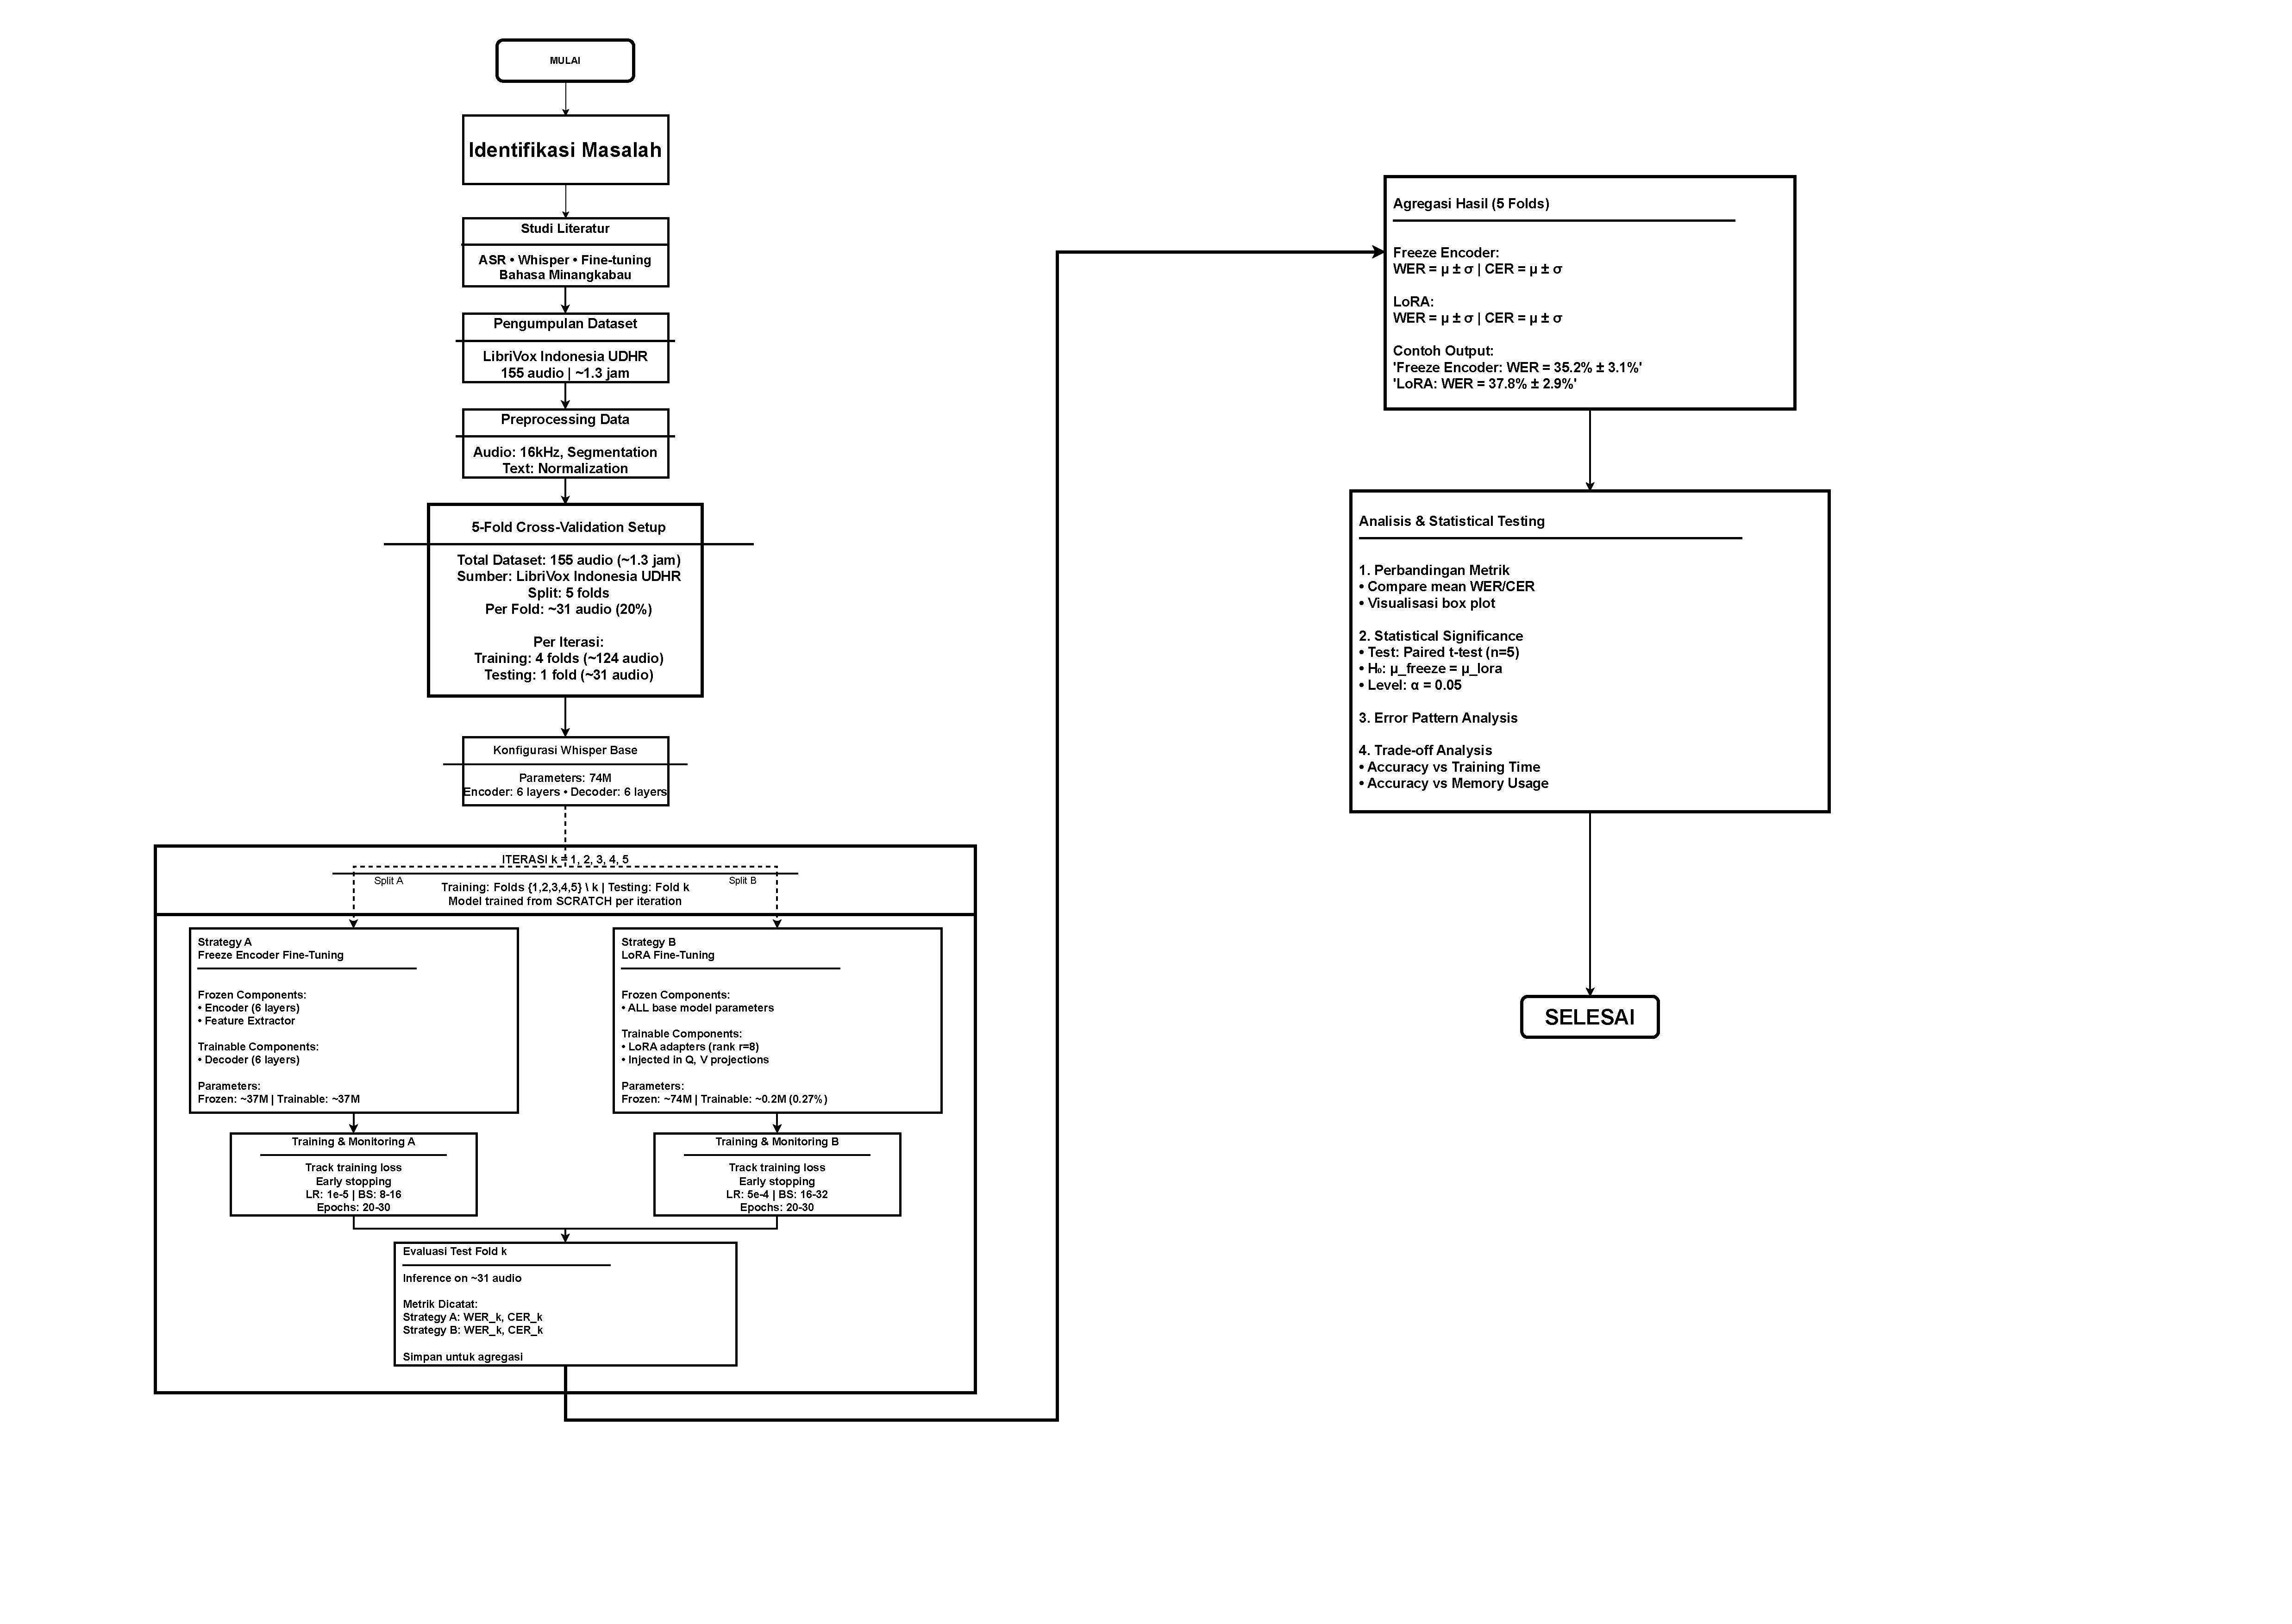
\includegraphics[width=0.6\textwidth]{figure/Alur_Penelitian.pdf}
\caption{Alur Penelitian Fine-Tuning Whisper untuk ASR Bahasa Minangkabau}
\label{fig:3.alur}
\end{figure}

\section{Penjabaran Langkah Penelitian}
\label{III.Jabar Alur}

Penelitian ini dilakukan secara sistematis melalui beberapa tahapan utama yang saling terkait. Setiap tahapan dirancang untuk memastikan model Whisper Small dapat diadaptasi secara optimal untuk mengenali bahasa Minangkabau. Berikut adalah penjabaran detail dari setiap langkah penelitian yang telah digambarkan pada flowchart di Subbab \ref{III.Alur}.

\subsection{Identifikasi Masalah}
\label{III.Langkah1}

Tahap pertama dalam alur penelitian ini adalah identifikasi masalah, yang dilakukan untuk memetakan konteks serta urgensi dari penelitian yang akan dilakukan. Proses ini diawali dengan analisis terhadap permasalahan di dunia nyata, yaitu rendahnya ketersediaan sistem \textit{Automatic Speech Recognition} (ASR) untuk bahasa daerah Indonesia, khususnya bahasa Minangkabau. Analisis ini divalidasi dengan meninjau statistik dan studi terkait yang menunjukkan bahwa sebagian besar sistem ASR komersial yang tersedia saat ini dirancang untuk bahasa-bahasa dengan sumber daya tinggi seperti bahasa Inggris, Mandarin, dan bahasa Eropa lainnya, sementara bahasa daerah Nusantara masih sangat terbatas representasinya.

Setelah urgensi masalah teridentifikasi, proses dilanjutkan dengan menganalisis tantangan spesifik yang dihadapi dalam pengembangan ASR untuk bahasa \textit{low-resource} seperti Minangkabau. Hasil analisis menemukan bahwa tantangan utama terletak pada minimnya ketersediaan dataset audio-transkrip berkualitas tinggi yang diperlukan untuk melatih model ASR. Kondisi ini berbeda dengan bahasa-bahasa besar yang memiliki ribuan jam data audio teranotasi. Identifikasi tantangan \textit{low-resource} ini menegaskan kebutuhan akan pendekatan yang efisien, sehingga penelitian ini difokuskan pada pemanfaatan model \textit{pre-trained} seperti Whisper yang telah dilatih pada skala besar dan dapat diadaptasi untuk bahasa target dengan data yang relatif terbatas.

Berdasarkan analisis tersebut, penelitian ini merumuskan \textit{research gap} yang jelas: belum ada penelitian yang secara komprehensif membandingkan strategi \textit{fine-tuning} yang berbeda (\textit{Full Fine-Tuning} vs LoRA) untuk adaptasi Whisper pada bahasa Minangkabau. Identifikasi masalah ini mencakup beberapa aspek kunci berikut:

\begin{enumerate}[noitemsep]
    \item Analisis keterbatasan sistem ASR \textit{existing} untuk bahasa daerah Indonesia, khususnya dari perspektif ketersediaan model dan dataset
    \item Identifikasi tantangan bahasa \textit{low-resource}: minimnya dataset audio-transkrip Minangkabau yang berkualitas dan teranotasi
    \item Perumusan \textit{research gap}: perlunya adaptasi model \textit{pre-trained} (Whisper) untuk bahasa Minangkabau dengan pendekatan yang efisien secara komputasi
    \item Penetapan objektif penelitian: membandingkan efektivitas strategi \textit{fine-tuning} (\textit{Full Fine-Tuning} vs LoRA) dalam hal akurasi dan efisiensi
    \item Penentuan metrik evaluasi utama: \textit{Word Error Rate} (WER) dan \textit{Character Error Rate} (CER) sebagai indikator kinerja model
\end{enumerate}

\subsection{Studi Literatur}
\label{III.Langkah2}

Setelah masalah utama teridentifikasi, langkah selanjutnya dalam alur penelitian adalah melakukan studi literatur secara sistematis dan komprehensif. Proses ini bertujuan untuk memvalidasi \textit{research gap} yang telah diidentifikasi pada tahap sebelumnya, mengumpulkan landasan teori yang relevan, serta memetakan metode \textit{state-of-the-art} yang akan digunakan sebagai dasar perbandingan dalam penelitian ini. Studi literatur dilakukan dengan pendekatan yang terstruktur untuk memastikan bahwa semua aspek penting dari penelitian tercakup dengan baik.

Studi literatur difokuskan pada empat area utama yang saling berkaitan. Pertama, mendalami arsitektur dan kemampuan model Whisper dari OpenAI, termasuk mekanisme \textit{encoder-decoder Transformer}, proses \textit{pre-training} pada 680,000 jam data multibahasa, dan karakteristik yang membuat Whisper unggul dalam skenario \textit{zero-shot} maupun \textit{few-shot}. Kedua, mengidentifikasi dan menganalisis strategi \textit{fine-tuning} yang telah terbukti efektif untuk bahasa \textit{low-resource}, dengan fokus khusus pada perbandingan antara \textit{Full Fine-Tuning} yang meng-\textit{update} seluruh parameter model versus teknik \textit{Parameter-Efficient Fine-Tuning} (PEFT) seperti LoRA yang hanya melatih sebagian kecil parameter. Ketiga, mempelajari penelitian-penelitian terdahulu yang telah menerapkan Whisper atau model ASR lainnya pada bahasa Indonesia dan bahasa daerah Nusantara, untuk memahami tantangan spesifik dan solusi yang telah dicoba. Keempat, memahami karakteristik linguistik bahasa Minangkabau, termasuk fonologi, morfologi, dan pola ucapan yang dapat mempengaruhi performa model ASR.

Proses studi literatur dilaksanakan melalui tahapan-tahapan berikut:

\begin{enumerate}[noitemsep]
    \item \textit{Review} paper ilmiah terkait Whisper dan strategi \textit{fine-tuning} dari jurnal internasional bereputasi (\textit{e.g.}, ICASSP, Interspeech, ACL) dan \textit{conference proceedings} di bidang \textit{speech processing}
    \item Analisis mendalam terhadap penelitian terdahulu tentang ASR untuk bahasa Indonesia dan bahasa daerah Nusantara, dengan fokus pada metodologi, dataset yang digunakan, dan hasil yang dicapai
    \item Studi dokumentasi teknis OpenAI Whisper dan ekosistem Hugging Face Transformers \textit{library}, termasuk \textit{API reference}, \textit{model cards}, dan \textit{best practices} untuk \textit{fine-tuning}
    \item Eksplorasi metode \textit{fine-tuning} yang tersedia, membandingkan karakteristik \textit{full fine-tuning} dengan pendekatan PEFT seperti LoRA, Adapter, dan Prefix-Tuning
    \item Pemahaman mendalam tentang metrik evaluasi ASR, khususnya \textit{Word Error Rate} (WER) dan \textit{Character Error Rate} (CER), termasuk interpretasi dan keterbatasannya
\end{enumerate}

Hasil dari studi literatur ini menjadi landasan teoritis yang kokoh dalam memilih arsitektur model, menentukan strategi \textit{fine-tuning} yang optimal, dan merancang metodologi evaluasi yang tepat untuk penelitian ini. Selain itu, studi literatur juga mengonfirmasi validitas \textit{research gap} yang telah diidentifikasi dan memberikan justifikasi ilmiah untuk pendekatan yang diusulkan.

\subsection{Pengumpulan Dataset}
\label{III.Langkah3}

Penelitian ini menggunakan dataset publik LibriVox Indonesia versi 1.0, yang merupakan koleksi rekaman audio dari buku-buku domain publik dalam berbagai bahasa daerah Indonesia. Secara spesifik, dataset bahasa Minangkabau yang digunakan berisi rekaman pembacaan \textit{Universal Declaration of Human Rights} (Pernyataan Umum tentang Hak-Hak Asasi Manusia) dalam bahasa Minangkabau. Pemilihan dataset LibriVox Indonesia sebagai sumber data didasarkan pada beberapa pertimbangan penting. Pertama, LibriVox menyediakan audio dengan kualitas rekaman yang relatif baik karena mengikuti standar produksi \textit{audiobook} dengan \textit{sampling rate} 44.1 kHz. Kedua, setiap audio dilengkapi dengan transkrip teks yang akurat karena dibacakan dari naskah tertulis (teks UDHR), sehingga mengurangi beban anotasi manual dan menjamin akurasi transkrip. Ketiga, dataset ini tersedia secara publik dengan lisensi \textit{Public Domain} (CC-0), memungkinkan penggunaan bebas untuk penelitian akademis.

Proses pengumpulan dataset dirancang secara sistematis menggunakan \textit{forced alignment software} yang dikembangkan oleh kontributor LibriVox Indonesia untuk mengkonversi rekaman \textit{audiobook} panjang menjadi segmen-segmen pendek yang sesuai untuk pelatihan ASR. Tahap awal dimulai dengan mengunduh dataset bahasa Minangkabau dari repositori LibriVox Indonesia melalui platform Hugging Face Datasets. Setelah dataset diunduh, dilakukan proses verifikasi kualitas untuk memastikan bahwa setiap segmen audio memiliki kejernihan ucapan yang baik (\textit{clear speech}), minim \textit{background noise}, dan tidak mengandung distorsi audio yang signifikan. Dataset LibriVox Indonesia telah melalui proses segmentasi otomatis yang membagi rekaman panjang menjadi klip-klip pendek dengan durasi beberapa detik hingga maksimal 20 detik, yang ideal untuk pelatihan model ASR.

Dataset bahasa Minangkabau dalam LibriVox Indonesia 1.0 mencakup total sekitar 8 jam rekaman audio dari 7 bahasa Indonesia yang berbeda, dengan porsi spesifik untuk bahasa Minangkabau yang akan digunakan dalam penelitian ini. Meskipun konten terbatas pada pembacaan UDHR, dataset ini tetap mencakup keberagaman \textit{speaker} dengan variasi karakteristik suara yang berbeda. Proses pengumpulan dan persiapan dataset mencakup langkah-langkah berikut:

\begin{enumerate}[noitemsep]
    \item Mengunduh dataset LibriVox Indonesia 1.0 dari Hugging Face Datasets, dengan fokus pada subset bahasa Minangkabau yang berisi pembacaan UDHR
    \item Verifikasi kualitas audio secara teknis untuk setiap segmen: \textit{clear speech}, minimal \textit{background noise}, tidak ada distorsi atau \textit{clipping}
    \item Validasi transkrip teks yang sesuai dengan setiap segmen audio, memastikan akurasi dan kelengkapan transkrip berdasarkan teks UDHR dalam bahasa Minangkabau
    \item Ekstraksi metadata \textit{speaker} (\\textit{reader ID}) untuk analisis keberagaman pembicara dalam dataset
    \item Inventarisasi total durasi audio yang tersedia dan perencanaan penggunaan data untuk mencapai cakupan yang memadai bagi proses \textit{fine-tuning}
\end{enumerate}

Dataset yang berhasil dikumpulkan dari LibriVox Indonesia mencakup rekaman pembacaan UDHR dalam bahasa Minangkabau, yang meskipun terbatas pada satu jenis teks (dokumen deklarasi HAM), tetap merepresentasikan bahasa Minangkabau formal dan standar. Karakteristik dataset ini sesuai untuk penelitian \textit{fine-tuning} model ASR pada bahasa \textit{low-resource}, di mana ketersediaan data yang terbatas merupakan tantangan utama yang perlu diatasi melalui pendekatan \textit{transfer learning} dari model \textit{pre-trained} seperti Whisper.

\subsection{Preprocessing Dataset}
\label{III.Langkah4}

Dataset mentah yang telah dikumpulkan akan melalui tahapan \textit{preprocessing} yang sistematis dan komprehensif untuk memastikan kompatibilitas dengan persyaratan teknis model Whisper serta mengoptimalkan kualitas data yang akan digunakan dalam proses \textit{fine-tuning}. \textit{Preprocessing} merupakan tahap kritis dalam penelitian ini karena kualitas dan konsistensi data input secara langsung mempengaruhi kinerja model ASR yang dilatih. Model Whisper memiliki spesifikasi teknis tertentu, terutama terkait format audio input, yang harus dipenuhi agar model dapat berfungsi secara optimal. Selain itu, \textit{preprocessing} juga bertujuan untuk standardisasi data sehingga mengurangi variabilitas yang tidak relevan dan memungkinkan model fokus pada pembelajaran pola linguistik yang penting.

Proses \textit{preprocessing} dirancang dalam tiga tahap utama yang saling melengkapi: \textit{audio preprocessing}, \textit{text preprocessing}, dan \textit{dataset splitting}. Setiap tahap memiliki tujuan spesifik dan menggunakan teknik-teknik yang telah terbukti efektif dalam penelitian ASR sebelumnya. Pendekatan sistematis ini memastikan bahwa dataset yang dihasilkan memiliki kualitas yang konsisten, kompatibel dengan arsitektur Whisper, dan siap digunakan untuk proses \textit{training}, \textit{validation}, dan \textit{testing}.

\subsubsection{Audio Preprocessing}

Tahap \textit{audio preprocessing} berfokus pada transformasi sinyal audio mentah menjadi format yang sesuai dengan spesifikasi teknis Whisper dan mengoptimalkan kualitas sinyal untuk pembelajaran model. Proses ini mencakup beberapa operasi penting:

\begin{enumerate}[noitemsep]
    \item \textbf{Format Conversion}: Konversi format audio dari MP3 (format asli LibriVox Indonesia) ke WAV (\textit{Waveform Audio File Format}). Konversi ini diperlukan karena format MP3 yang terkompresi dengan \textit{lossy compression} memerlukan proses \textit{decoding} tambahan yang dapat membebani komputasi Whisper. Format WAV yang \textit{uncompressed} memungkinkan akses langsung ke data audio mentah (\textit{raw audio samples}), sehingga mengurangi beban komputasi dan mempercepat proses \textit{preprocessing} serta \textit{training}
    \item \textbf{Resampling}: Konversi \textit{sampling rate} audio dari 44.1 kHz (format asli LibriVox Indonesia) ke 16 kHz, yang merupakan spesifikasi standar yang digunakan oleh model Whisper. Konversi ini penting karena model Whisper dilatih dengan data audio pada frekuensi 16 kHz dan akan menghasilkan performa optimal pada \textit{sampling rate} yang sama
    \item \textbf{Segmentation}: Pemotongan audio panjang menjadi \textit{clips} dengan durasi 10-30 detik untuk meningkatkan efisiensi \textit{training} dan mengurangi penggunaan memori GPU. Segmentasi juga membantu model mempelajari pola dalam konteks yang lebih terfokus
    \item \textbf{Normalization}: Normalisasi \textit{amplitude} audio untuk memastikan konsistensi volume di seluruh dataset, menghindari bias model terhadap audio dengan volume tertentu
    \item \textbf{Silence Removal}: Penghapusan periode \textit{silence} yang tidak informatif di awal dan akhir setiap \textit{clip}, sehingga model tidak perlu memproses bagian audio yang tidak mengandung informasi linguistik
    \item \textbf{Quality Check}: Penyaringan \textit{clips} dengan \textit{Signal-to-Noise Ratio} (SNR) rendah atau mengandung distorsi signifikan, untuk memastikan hanya data berkualitas tinggi yang digunakan dalam \textit{training}
\end{enumerate}

\subsubsection{Text Preprocessing}

Tahap \textit{text preprocessing} bertujuan untuk menstandarkan transkrip teks dan menghilangkan variasi yang tidak relevan untuk tugas ASR. Standarisasi teks penting untuk memastikan konsistensi dalam pelatihan model dan evaluasi hasil. Proses ini mencakup:

\begin{enumerate}[noitemsep]
    \item \textbf{Lowercase Conversion}: Konversi semua teks ke huruf kecil untuk mengurangi ukuran \textit{vocabulary} dan menghilangkan perbedaan yang tidak relevan antara kapitalisasi
    \item \textbf{Punctuation Normalization}: Standarisasi tanda baca untuk konsistensi format, termasuk normalisasi tanda kutip, tanda hubung, dan simbol-simbol khusus
    \item \textbf{Number Normalization}: Konversi representasi numerik menjadi bentuk kata (\textit{e.g.}, "10" $\rightarrow$ "sepuluh", "2025" $\rightarrow$ "dua ribu dua puluh lima") untuk konsistensi dengan bagaimana angka diucapkan dalam bahasa Minangkabau
    \item \textbf{Whitespace Normalization}: Pembersihan spasi berlebih, tab, dan karakter \textit{whitespace} lainnya untuk memastikan format teks yang konsisten
    \item \textbf{Special Character Handling}: Penanganan khusus untuk karakter-karakter yang spesifik dalam bahasa Minangkabau, termasuk diakritik atau simbol yang mungkin muncul dalam transkrip
\end{enumerate}

\subsubsection{Dataset Splitting}

Setelah \textit{preprocessing} audio dan teks selesai, dataset dibagi menjadi tiga subset dengan proporsi yang standar dalam penelitian \textit{machine learning}:

\begin{itemize}[noitemsep]
    \item \textit{Training set}: 80\% dari total data, digunakan untuk melatih parameter model
    \item \textit{Validation set}: 10\% dari total data, digunakan untuk memantau performa selama \textit{training} dan melakukan \textit{hyperparameter tuning}
    \item \textit{Test set}: 10\% dari total data, digunakan untuk evaluasi final dan tidak pernah dilihat oleh model selama \textit{training}
\end{itemize}

Pembagian dilakukan secara \textit{stratified} untuk memastikan distribusi \textit{speaker}, dialek Minangkabau, dan karakteristik lainnya seimbang di setiap subset. Pendekatan \textit{stratified splitting} ini penting untuk menghindari bias dalam evaluasi dan memastikan bahwa setiap subset merepresentasikan keberagaman yang ada dalam dataset lengkap.

\subsection{Konfigurasi Model Whisper Small}
\label{III.Langkah5}

Model Whisper Small dipilih sebagai arsitektur \textit{base model} dalam penelitian ini berdasarkan pertimbangan yang cermat terhadap \textit{trade-off} antara performa, efisiensi komputasi, dan kelayakan untuk skenario \textit{low-resource}. Whisper Small, dengan 244 juta parameter, merupakan varian menengah dari keluarga model Whisper yang menawarkan keseimbangan optimal: cukup besar untuk menangkap kompleksitas bahasa tetapi tidak terlalu besar sehingga memerlukan sumber daya komputasi yang tidak realistis untuk \textit{fine-tuning} pada infrastruktur \textit{cloud} yang tersedia seperti RunPod. Pemilihan ini juga didukung oleh studi-studi sebelumnya yang menunjukkan bahwa Whisper Small dapat mencapai performa yang kompetitif pada berbagai tugas ASR, terutama setelah di-\textit{fine-tune} pada bahasa target.

Arsitektur Whisper Small menggunakan \textit{encoder-decoder Transformer} dengan konfigurasi yang telah dioptimalkan untuk tugas \textit{speech recognition}. Model ini telah di-\textit{pre-train} pada dataset multibahasa yang sangat besar (680,000 jam audio) sehingga memiliki representasi yang kuat tentang pola akustik dan linguistik lintas bahasa. Karakteristik \textit{pre-trained} ini memungkinkan model untuk di-\textit{transfer} dengan efisien ke bahasa Minangkabau meskipun dengan data \textit{fine-tuning} yang relatif terbatas (10-20 jam). Proses konfigurasi model dilakukan secara sistematis untuk memastikan semua komponen berfungsi dengan benar dan siap untuk tahap \textit{fine-tuning}.

Tahap konfigurasi model Whisper Small mencakup beberapa langkah teknis penting:

\begin{enumerate}[noitemsep]
    \item \textit{Loading pre-trained} Whisper Small (244M \textit{parameters}) dari Hugging Face Model Hub menggunakan \textit{library} Transformers, memastikan model dalam keadaan \textit{pre-trained} yang telah terbukti efektif
    \item Verifikasi arsitektur model: 12 \textit{encoder layers} dan 12 \textit{decoder layers}, dengan \textit{hidden dimension} (\textit{width}) 768 dan 12 \textit{attention heads} per \textit{layer}, sesuai dengan spesifikasi resmi Whisper Small
    \item Inisialisasi \textit{tokenizer} dengan \textit{vocabulary} sebesar 51,864 \textit{tokens}, yang mencakup representasi karakter dan subword untuk berbagai bahasa termasuk kemampuan untuk mengakomodasi bahasa baru
    \item Konfigurasi \textit{feature extractor} untuk menghasilkan representasi \textit{log-Mel spectrogram} dengan 80 dimensi, menggunakan \textit{window size} 25ms dan \textit{hop length} 10ms, yang merupakan parameter standar untuk ekstraksi fitur audio dalam Whisper
    \item \textit{Setup device} (GPU/CPU) untuk \textit{training}, dengan preferensi GPU (NVIDIA GeForce RTX 4090 dengan 24 GB VRAM) untuk mempercepat komputasi matriks dalam proses \textit{fine-tuning}
\end{enumerate}

\subsection{Implementasi Fine-Tuning}
\label{III.Langkah6}

Penelitian ini menerapkan pendekatan komparatif dengan membandingkan dua strategi \textit{fine-tuning} yang berbeda: \textit{Full Fine-Tuning} dan \textit{Low-Rank Adaptation} (LoRA). Pemilihan kedua strategi ini didasarkan pada karakteristik yang saling melengkapi dalam konteks bahasa \textit{low-resource}. \textit{Full Fine-Tuning} merepresentasikan pendekatan tradisional yang meng-\textit{update} seluruh parameter model, berpotensi menghasilkan adaptasi yang paling optimal tetapi dengan biaya komputasi yang tinggi. Sebaliknya, LoRA merupakan teknik \textit{Parameter-Efficient Fine-Tuning} (PEFT) yang hanya melatih sebagian kecil parameter tambahan, menawarkan efisiensi komputasi yang signifikan dengan trade-off minimal dalam akurasi. Implementasi kedua metode dilakukan secara terpisah dan sistematis untuk memastikan perbandingan yang adil dan valid.

Pendekatan komparatif ini memungkinkan analisis mendalam terhadap \textit{trade-off} antara akurasi model dan efisiensi sumber daya. Dalam konteks bahasa Minangkabau sebagai bahasa \textit{low-resource}, pertanyaan penting yang perlu dijawab adalah: apakah efisiensi LoRA (dengan hanya melatih $\sim$2\% parameter) memberikan hasil yang sebanding dengan \textit{Full Fine-Tuning} (yang melatih 100\% parameter)? Jika LoRA dapat mencapai performa yang mendekati \textit{Full Fine-Tuning} dengan biaya komputasi yang jauh lebih rendah, maka LoRA menjadi solusi yang lebih praktis dan dapat diskalakan untuk bahasa-bahasa \textit{low-resource} lainnya. Untuk menjawab pertanyaan ini, implementasi kedua metode dirancang dengan cermat dengan pengaturan \textit{hyperparameter} yang dioptimalkan untuk masing-masing pendekatan.

\subsubsection{Full Fine-Tuning}

Pada metode \textit{Full Fine-Tuning}, seluruh 244 juta parameter model Whisper Small di-\textit{update} selama proses \textit{training}. Pendekatan ini memberikan fleksibilitas maksimal bagi model untuk beradaptasi dengan karakteristik spesifik bahasa Minangkabau, termasuk pola fonetik, intonasi, dan struktur linguistik yang unik. Konfigurasi \textit{training} untuk \textit{Full Fine-Tuning} adalah sebagai berikut:

\begin{enumerate}[noitemsep]
    \item \textbf{Optimizer}: AdamW (\textit{Adam with Weight Decay}) dengan \textit{weight decay} 0.01 untuk regularisasi dan mencegah \textit{overfitting}
    \item \textbf{Learning Rate}: $2 \times 10^{-5}$ dengan strategi \textit{linear warmup} (500 langkah) diikuti \textit{cosine decay} untuk konvergensi yang stabil
    \item \textbf{Batch Size}: 16 sampel per \textit{batch}, dengan opsi \textit{gradient accumulation} jika memori GPU tidak mencukupi
    \item \textbf{Epochs}: 10-15 \textit{epochs} dengan mekanisme \textit{early stopping} (\textit{patience}=5) untuk menghentikan \textit{training} jika tidak ada peningkatan pada \textit{validation} WER
    \item \textbf{Loss Function}: \textit{Cross-entropy loss} standar untuk tugas klasifikasi sekuens
\end{enumerate}

\subsubsection{LoRA Fine-Tuning}

Metode LoRA (\textit{Low-Rank Adaptation}) bekerja dengan menambahkan matriks \textit{low-rank} sebagai parameter yang dapat dilatih pada \textit{attention layers}, sementara seluruh parameter \textit{pre-trained} dari Whisper Small tetap \textit{frozen}. Pendekatan ini sangat efisien karena hanya melatih $\sim$2\% dari total parameter (sekitar 5 juta parameter dari 244 juta), namun tetap mampu mencapai performa yang kompetitif. Konfigurasi LoRA \textit{fine-tuning} adalah sebagai berikut:

\begin{enumerate}[noitemsep]
    \item \textbf{LoRA Configuration}:
    \begin{itemize}[noitemsep]
        \item \textit{Rank} ($r$): 8 (dimensi matriks \textit{low-rank} yang ditambahkan)
        \item \textit{Alpha}: 16 (\textit{scaling factor} untuk LoRA \textit{updates})
        \item \textit{Dropout}: 0.1 (regularisasi pada LoRA \textit{layers})
        \item \textit{Target modules}: \textit{Query} dan \textit{Value projections} dalam \textit{attention layers}, yang merupakan komponen paling kritis untuk adaptasi
    \end{itemize}
    \item \textbf{Trainable Parameters}: $\sim$2\% dari total parameter ($\sim$5 juta parameter), drastis lebih sedikit dibanding \textit{Full Fine-Tuning}
    \item \textbf{Optimizer}: AdamW dengan \textit{weight decay} 0.01
    \item \textbf{Learning Rate}: $5 \times 10^{-4}$ (lebih tinggi dibanding \textit{Full FT} karena hanya melatih sebagian kecil parameter pada \textit{frozen base model})
    \item \textbf{Batch Size}: 16 sampel per \textit{batch}
    \item \textbf{Epochs}: 10-15 \textit{epochs} dengan \textit{early stopping} (\textit{patience}=5)
\end{enumerate}

\subsubsection{Data Augmentation}

Untuk meningkatkan \textit{robustness} model pada skenario \textit{low-resource} dan mencegah \textit{overfitting} pada dataset yang relatif kecil, diterapkan beberapa teknik \textit{data augmentation} pada data audio selama \textit{training}:

\begin{enumerate}[noitemsep]
    \item \textbf{SpecAugment}: Teknik \textit{augmentation} pada representasi spektrogram dengan menerapkan \textit{time masking} (T=70) dan \textit{frequency masking} (F=27) untuk meningkatkan invariansi temporal dan frekuensi
    \item \textbf{Speed Perturbation}: Variasi kecepatan audio dengan faktor $\{0.9, 1.0, 1.1\}$ untuk mensimulasikan variasi kecepatan bicara alami
    \item \textbf{Noise Injection}: Penambahan \textit{environmental noise} dengan SNR 15-25 dB untuk meningkatkan \textit{robustness} model terhadap kondisi audio yang beragam
\end{enumerate}

\subsubsection{Regularization}

Selain \textit{data augmentation}, beberapa teknik \textit{regularization} juga diterapkan untuk mencegah \textit{overfitting} dan meningkatkan generalisasi model:

\begin{enumerate}[noitemsep]
    \item \textit{Dropout} pada \textit{attention layers} (p=0.1) dan \textit{feed-forward network} (FFN) \textit{layers} (p=0.3) untuk mengurangi \textit{co-adaptation} antar \textit{neurons}
    \item \textit{Label smoothing} ($\epsilon = 0.1$) untuk mencegah overconfidence pada prediksi dan meningkatkan kalibrasi model
    \item \textit{Gradient clipping} (\textit{max norm} = 1.0) untuk mencegah \textit{exploding gradients} selama \textit{training}
    \item \textit{Early stopping} berdasarkan \textit{validation} WER, menghentikan \textit{training} jika tidak ada perbaikan selama 5 \textit{epochs} berturut-turut
\end{enumerate}

\subsection{Training dan Monitoring}
\label{III.Langkah7}

Proses \textit{training} dilakukan dengan protokol \textit{monitoring} yang ketat dan sistematis untuk memastikan konvergensi yang optimal serta mendeteksi potensi masalah sejak dini. \textit{Monitoring} yang komprehensif sangat penting dalam penelitian ini mengingat kompleksitas model Whisper dan sifat dataset yang \textit{low-resource}. Tanpa \textit{monitoring} yang tepat, berbagai masalah seperti \textit{overfitting}, konvergensi yang lambat, atau konfigurasi \textit{hyperparameter} yang tidak optimal dapat tidak terdeteksi dan menghasilkan model dengan performa suboptimal. Oleh karena itu, strategi \textit{monitoring} dirancang untuk memberikan visibilitas penuh terhadap seluruh aspek proses \textit{training}, dari metrik performa hingga penggunaan sumber daya komputasi.

Infrastruktur \textit{training} menggunakan RunPod \textit{Cloud GPU Service} dengan NVIDIA GeForce RTX 4090 (24 GB VRAM), yang menyediakan performa komputasi tinggi untuk \textit{fine-tuning} model berukuran menengah seperti Whisper Small. Seluruh proses \textit{training} untuk kedua strategi (\textit{Full Fine-Tuning} dan LoRA) dilakukan pada infrastruktur yang sama untuk memastikan perbandingan yang adil. Metrik-metrik kunci dicatat secara otomatis menggunakan \textit{logging framework} yang terintegrasi, dan \textit{checkpointing} dilakukan secara berkala untuk menyimpan \textit{state} model terbaik.

Protokol \textit{training} dan \textit{monitoring} yang diterapkan mencakup aspek-aspek berikut:

\begin{enumerate}[noitemsep]
    \item \textit{Training} dilakukan pada RunPod dengan akselerasi GPU NVIDIA GeForce RTX 4090 (24 GB VRAM) untuk mempercepat komputasi matriks dalam \textit{backpropagation}
    \item \textit{Logging} metrik setiap 100 \textit{steps}: \textit{training loss}, \textit{learning rate} saat ini, dan waktu komputasi per \textit{batch}, untuk memantau progres \textit{training} secara real-time
    \item Evaluasi pada \textit{validation set} setiap \textit{epoch}: perhitungan WER, CER, dan \textit{validation loss} untuk memantau kemampuan generalisasi model
    \item \textit{Checkpoint} model terbaik berdasarkan \textit{lowest validation} WER, memastikan model yang disimpan adalah yang paling optimal untuk tugas ASR bahasa Minangkabau
    \item \textit{Tracking training time} dan penggunaan memori GPU untuk analisis efisiensi komputasi, terutama penting untuk membandingkan \textit{Full Fine-Tuning} dengan LoRA
    \item Visualisasi \textit{learning curves} (\textit{loss}, WER, CER vs \textit{epochs}) menggunakan \textit{TensorBoard} atau \textit{Weights \& Biases} untuk analisis visual terhadap konvergensi model
\end{enumerate}

\subsection{Evaluasi Model}
\label{III.Langkah8}

Model yang telah di-\textit{fine-tune} dievaluasi secara komprehensif menggunakan \textit{test set} yang tidak pernah dilihat oleh model selama proses \textit{training} maupun \textit{validation}. Prinsip isolasi \textit{test set} ini sangat penting untuk memastikan bahwa metrik evaluasi yang diperoleh merepresentasikan kemampuan generalisasi model yang sebenarnya pada data baru, bukan hanya kemampuan menghafal pola dalam data \textit{training}. Evaluasi dilakukan dengan protokol yang konsisten untuk kedua strategi \textit{fine-tuning} (\textit{Full Fine-Tuning} dan LoRA) untuk memungkinkan perbandingan yang adil dan valid.

Proses evaluasi dirancang untuk mengukur berbagai aspek performa model, tidak hanya akurasi transkrip tetapi juga \textit{error patterns} dan karakteristik kesalahan yang terjadi. Analisis \textit{error patterns} memberikan \textit{insights} penting tentang jenis kesalahan yang paling sering dibuat model (substitusi, penghapusan, atau penyisipan kata), yang dapat menjadi dasar untuk perbaikan model di masa depan. Selain itu, evaluasi juga mempertimbangkan variasi dialek Minangkabau jika memungkinkan, untuk memahami seberapa baik model dapat menangani keberagaman linguistik dalam bahasa target.

Protokol evaluasi yang diterapkan mencakup tahapan-tahapan berikut:

\begin{enumerate}[noitemsep]
    \item \textit{Inference} pada \textit{test set} menggunakan algoritma \textit{beam search} dengan \textit{beam size} = 5, yang memberikan keseimbangan antara kualitas transkrip dan kecepatan inferensi
    \item Perhitungan \textit{Word Error Rate} (WER) sebagai metrik utama untuk mengukur akurasi transkrip pada level kata
    \item Perhitungan \textit{Character Error Rate} (CER) sebagai metrik tambahan yang lebih sensitif terhadap kesalahan fonetik dan memberikan perspektif komplementer terhadap WER
    \item Normalisasi teks sebelum evaluasi (konversi ke \textit{lowercase}, penghapusan tanda baca, normalisasi\textit{whitespace}) untuk memastikan konsistensi dalam perhitungan metrik
    \item Analisis \textit{error patterns} detail dengan mengkategorikan kesalahan menjadi: substitusi (kata yang salah diganti), penghapusan (kata yang hilang), dan penyisipan (kata tambahan yang tidak seharusnya ada)
    \item Perbandingan performa antara model \textit{Full Fine-Tuning} dan LoRA menggunakan metrik WER, CER, serta analisis \textit{trade-off} dengan waktu \textit{training} dan penggunaan memori
    \item Evaluasi per-dialek Minangkabau (\textit{e.g.}, dialek Padang, Bukittinggi, Payakumbuh) jika distribusi data memungkinkan, untuk memahami kemampuan model menangani variasi linguistik
\end{enumerate}

\subsection{Analisis Hasil dan Perbandingan}
\label{III.Langkah9}

Tahap akhir dari alur penelitian adalah melakukan analisis mendalam terhadap hasil evaluasi dan membandingkan performa antara dua strategi \textit{fine-tuning} yang telah diimplementasikan. Analisis ini tidak hanya berfokus pada perbandingan metrik akurasi (WER dan CER), tetapi juga mempertimbangkan aspek-aspek praktis lainnya seperti efisiensi komputasi, waktu \textit{training}, penggunaan memori, dan kelayakan untuk deployment. Pendekatan analisis komparatif ini bertujuan untuk memberikan rekomendasi yang komprehensif dan berbasis bukti mengenai strategi \textit{fine-tuning} yang paling sesuai untuk adaptasi Whisper pada bahasa Minangkabau dan bahasa \textit{low-resource} lainnya.

Analisis dilakukan dengan mengintegrasikan evaluasi kuantitatif (metrik numerik) dan kualitatif (analisis transkrip), memberikan pemahaman yang holistik tentang kekuatan dan kelemahan masing-masing strategi. Evaluasi kuantitatif mencakup perbandingan statistik WER dan CER, sementara evaluasi kualitatif melibatkan inspeksi manual terhadap sampel transkrip untuk mengidentifikasi pola kesalahan yang mungkin tidak tertangkap oleh metrik numerik. Pendekatan ganda ini memastikan bahwa kesimpulan yang ditarik tidak hanya berdasarkan angka-angka tetapi juga didukung oleh pemahaman mendalam tentang perilaku model.

Proses analisis hasil dan perbandingan mencakup aspek-aspek berikut:

\begin{enumerate}[noitemsep]
    \item Perbandingan metrik WER dan CER antara \textit{Full Fine-Tuning} dan LoRA pada \textit{test set} yang sama, termasuk perhitungan selisih performa dan signifikansi statistik perbedaan tersebut
    \item Analisis \textit{trade-off} multidimensional: akurasi model vs efisiensi \textit{training} (waktu pelatihan, penggunaan memori GPU, jumlah parameter yang dilatih), untuk mengidentifikasi strategi yang menawarkan keseimbangan terbaik
    \item Evaluasi kualitas transkrip secara kualitatif melalui inspeksi manual terhadap sampel transkrip, mengidentifikasi jenis kesalahan yang paling umum dan konteks di mana setiap metode unggul atau lemah
    \item Identifikasi \textit{patterns of errors} yang spesifik (\textit{common misrecognitions}), seperti fonem atau kata Minangkabau yang sering salah dikenali, untuk memberikan \textit{insights} bagi penelitian lanjutan
    \item Analisis performa pada \textit{different speaking styles} (\textit{e.g.}, narasi formal vs informal) dan dialek Minangkabau yang berbeda, jika distribusi data memungkinkan
    \item Diskusi tentang \textit{limitations} penelitian (\textit{e.g.}, ukuran dataset yang terbatas, variasi dialek yang tidak sepenuhnya tercakup) dan \textit{potential improvements} untuk penelitian masa depan
    \item Perumusan rekomendasi strategi \textit{fine-tuning} terbaik untuk bahasa Minangkabau berdasarkan hasil analisis komprehensif, dengan pertimbangan terhadap konteks penggunaan (\textit{e.g.}, penelitian akademis vs aplikasi praktis)
\end{enumerate}

\section{Alat dan Bahan Tugas Akhir}
\label{III.Alat dan Bahan}

Penelitian ini memerlukan berbagai alat dan bahan untuk mendukung implementasi dan evaluasi model ASR bahasa Minangkabau.

\subsection{Alat}
\label{III.Alat}

Alat-alat yang digunakan dalam penelitian ini meliputi perangkat keras dan perangkat lunak:

\subsubsection{Perangkat Keras}

\begin{enumerate}[noitemsep]
    \item \textbf{Laptop}: ASUS VivoBook 14 K413 (11th Gen Intel), digunakan untuk \textit{development}, analisis data, dan penulisan kode
    \begin{itemize}[noitemsep]
        \item Processor: Intel Core i3 (11th Generation)
        \item RAM: 8 GB DDR4
        \item Storage: 512 GB SSD
        \item Sistem operasi: Linux/Windows
        \item Fungsi: \textit{Development environment}, eksplorasi data, dan analisis hasil
    \end{itemize}
    \item \textbf{RunPod Cloud GPU Service}: Platform \textit{cloud computing} untuk \textit{training} model dengan GPU
    \begin{itemize}[noitemsep]
        \item GPU: NVIDIA GeForce RTX 4090 (24 GB VRAM)
        \item RAM: 36 GB
        \item vCPU: 8 \textit{virtual cores}
        \item Storage: 80 GB \textit{disk space}
        \item Container: \texttt{runpod/pytorch:1.0.2-cu1281-torch280-ubuntu2404}
        \item Fungsi: \textit{Training} model \textit{Full Fine-Tuning} dan LoRA dengan akselerasi GPU
    \end{itemize}
\end{enumerate}

\subsubsection{Perangkat Lunak}

\begin{enumerate}[noitemsep]
    \item \textbf{Python 3.10+}: Bahasa pemrograman utama untuk implementasi model dan \textit{data processing}
    \item \textbf{PyTorch 2.8.0}: \textit{Deep learning framework} untuk \textit{training} dan \textit{inference} model Whisper
    \item \textbf{CUDA 12.8.1}: \textit{NVIDIA CUDA Toolkit} untuk akselerasi GPU pada RunPod
    \item \textbf{Ubuntu 24.04 LTS}: Sistem operasi \textit{Linux} pada \textit{container} RunPod (\texttt{runpod/pytorch:1.0.2-cu1281-torch280-ubuntu2404})
    \item \textbf{Hugging Face Transformers}: \textit{Library} untuk memuat dan \textit{fine-tune} model Whisper \textit{pre-trained}
    \item \textbf{Hugging Face Datasets}: \textit{Library} untuk manajemen dataset, \textit{data loading}, dan \textit{streaming} dari Hugging Face Hub
    \item \textbf{Hugging Face Accelerate}: \textit{Library} untuk \textit{distributed training}, optimisasi memori, dan akselerasi proses \textit{training} pada GPU
    \item \textbf{Hugging Face Evaluate}: \textit{Library} untuk evaluasi metrik model \textit{machine learning} secara standar dan konsisten
    \item \textbf{PEFT (Parameter-Efficient Fine-Tuning)}: \textit{Library} dari Hugging Face untuk implementasi LoRA dan metode \textit{fine-tuning} yang efisien parameter
    \item \textbf{torchaudio}: \textit{Library} PyTorch untuk \textit{audio processing}, transformasi, dan augmentasi data audio
    \item \textbf{torchcodec}: \textit{Library} untuk \textit{encoding} dan \textit{decoding} berbagai format audio dengan \textit{backend} PyTorch
    \item \textbf{audiomentations}: \textit{Library} untuk \textit{data augmentation} audio (\textit{noise injection}, \textit{pitch shifting}, \textit{time stretching})
    \item \textbf{jiwer}: \textit{Library} untuk perhitungan metrik evaluasi ASR (WER dan CER)
    \item \textbf{scikit-learn}: \textit{Library} untuk utilitas \textit{machine learning} (\textit{data splitting}, metrik evaluasi, \textit{preprocessing})
    \item \textbf{TensorBoard}: Platform visualisasi untuk \textit{monitoring} metrik \textit{training}, \textit{loss curves}, dan parameter model secara \textit{real-time}
    \item \textbf{Weights \& Biases (wandb)}: Platform untuk \textit{experiment tracking}, visualisasi \textit{learning curves}, perbandingan eksperimen, dan \textit{logging} metrik
    \item \textbf{Jupyter Notebook}: \textit{Interactive development environment} untuk eksplorasi data, eksperimen model, dan dokumentasi proses penelitian
    \item \textbf{Git/GitHub}: \textit{Version control system} dan repositori kode untuk manajemen proyek dan kolaborasi
    \item \textbf{Visual Studio Code}: \textit{Code editor} untuk \textit{local development} pada ASUS VivoBook 14 K413
\end{enumerate}

\subsection{Bahan}
\label{III.Bahan}

Bahan-bahan yang digunakan dalam penelitian ini meliputi dataset dan dokumen referensi:

\begin{enumerate}[noitemsep]
    \item \textbf{Dataset Audio Bahasa Minangkabau}:
    \begin{itemize}[noitemsep]
        \item Sumber: LibriVox Indonesia 1.0 via Hugging Face Datasets (\url{https://huggingface.co/datasets/indonesian-nlp/librivox-indonesia})
        \item Konten: Pembacaan \textit{Universal Declaration of Human Rights} dalam bahasa Minangkabau
        \item Format: Audio \textit{files} MP3 dengan \textit{sampling rate} 44.1 kHz
        \item Durasi: Sekitar 8 jam total (7 bahasa), subset Minangkabau digunakan untuk penelitian
        \item Segmentasi: Klip audio dengan durasi beberapa detik hingga maksimal 20 detik
        \item Lisensi: \textit{Public Domain} (CC-0)
    \end{itemize}
    \item \textbf{Model Pre-trained}:
    \begin{itemize}[noitemsep]
        \item Whisper Small dari OpenAI (via Hugging Face Model Hub)
        \item Model ID: \texttt{openai/whisper-small}
        \item Lisensi: MIT License
    \end{itemize}
    \item \textbf{Dokumen Referensi}:
    \begin{itemize}[noitemsep]
        \item Paper: "Robust Speech Recognition via Large-Scale Weak Supervision" \cite{radford2023whisper}
        \item Paper: "LoRA: Low-Rank Adaptation of Large Language Models" \cite{hu2022lora}
        \item Paper: "Exploration of Whisper Fine-Tuning Strategies for Low-Resource ASR" \cite{liu2024exploration}
        \item Dokumentasi Hugging Face Transformers
        \item Dokumentasi PEFT library
    \end{itemize}
\end{enumerate}

\section{Metode Pengembangan}
\label{III.Metode}

Penelitian ini menggunakan pendekatan eksperimental dengan metodologi yang terstruktur untuk memastikan validitas dan reproducibility hasil.

\subsection{Pendekatan Penelitian}
\label{III.Pendekatan}

Penelitian ini mengadopsi \textbf{pendekatan eksperimental} dengan karakteristik:

\begin{enumerate}[noitemsep]
    \item \textbf{Quantitative Evaluation}: Pengukuran performa menggunakan metrik objektif (WER, CER)
    \item \textbf{Comparative Study}: Perbandingan antara dua strategi fine-tuning (Full vs LoRA)
    \item \textbf{Controlled Experiment}: Dataset, hyperparameters, dan evaluation protocol dijaga konsisten
    \item \textbf{Reproducible Research}: Semua kode, konfigurasi, dan hasil didokumentasikan
\end{enumerate}

\subsection{Alur Pengembangan}
\label{III.Alur_Pengembangan}

Pengembangan sistem ASR bahasa Minangkabau mengikuti alur yang sistematis seperti digambarkan pada Gambar \ref{fig:3.alur_dev}:

\begin{figure}[H]
\centering
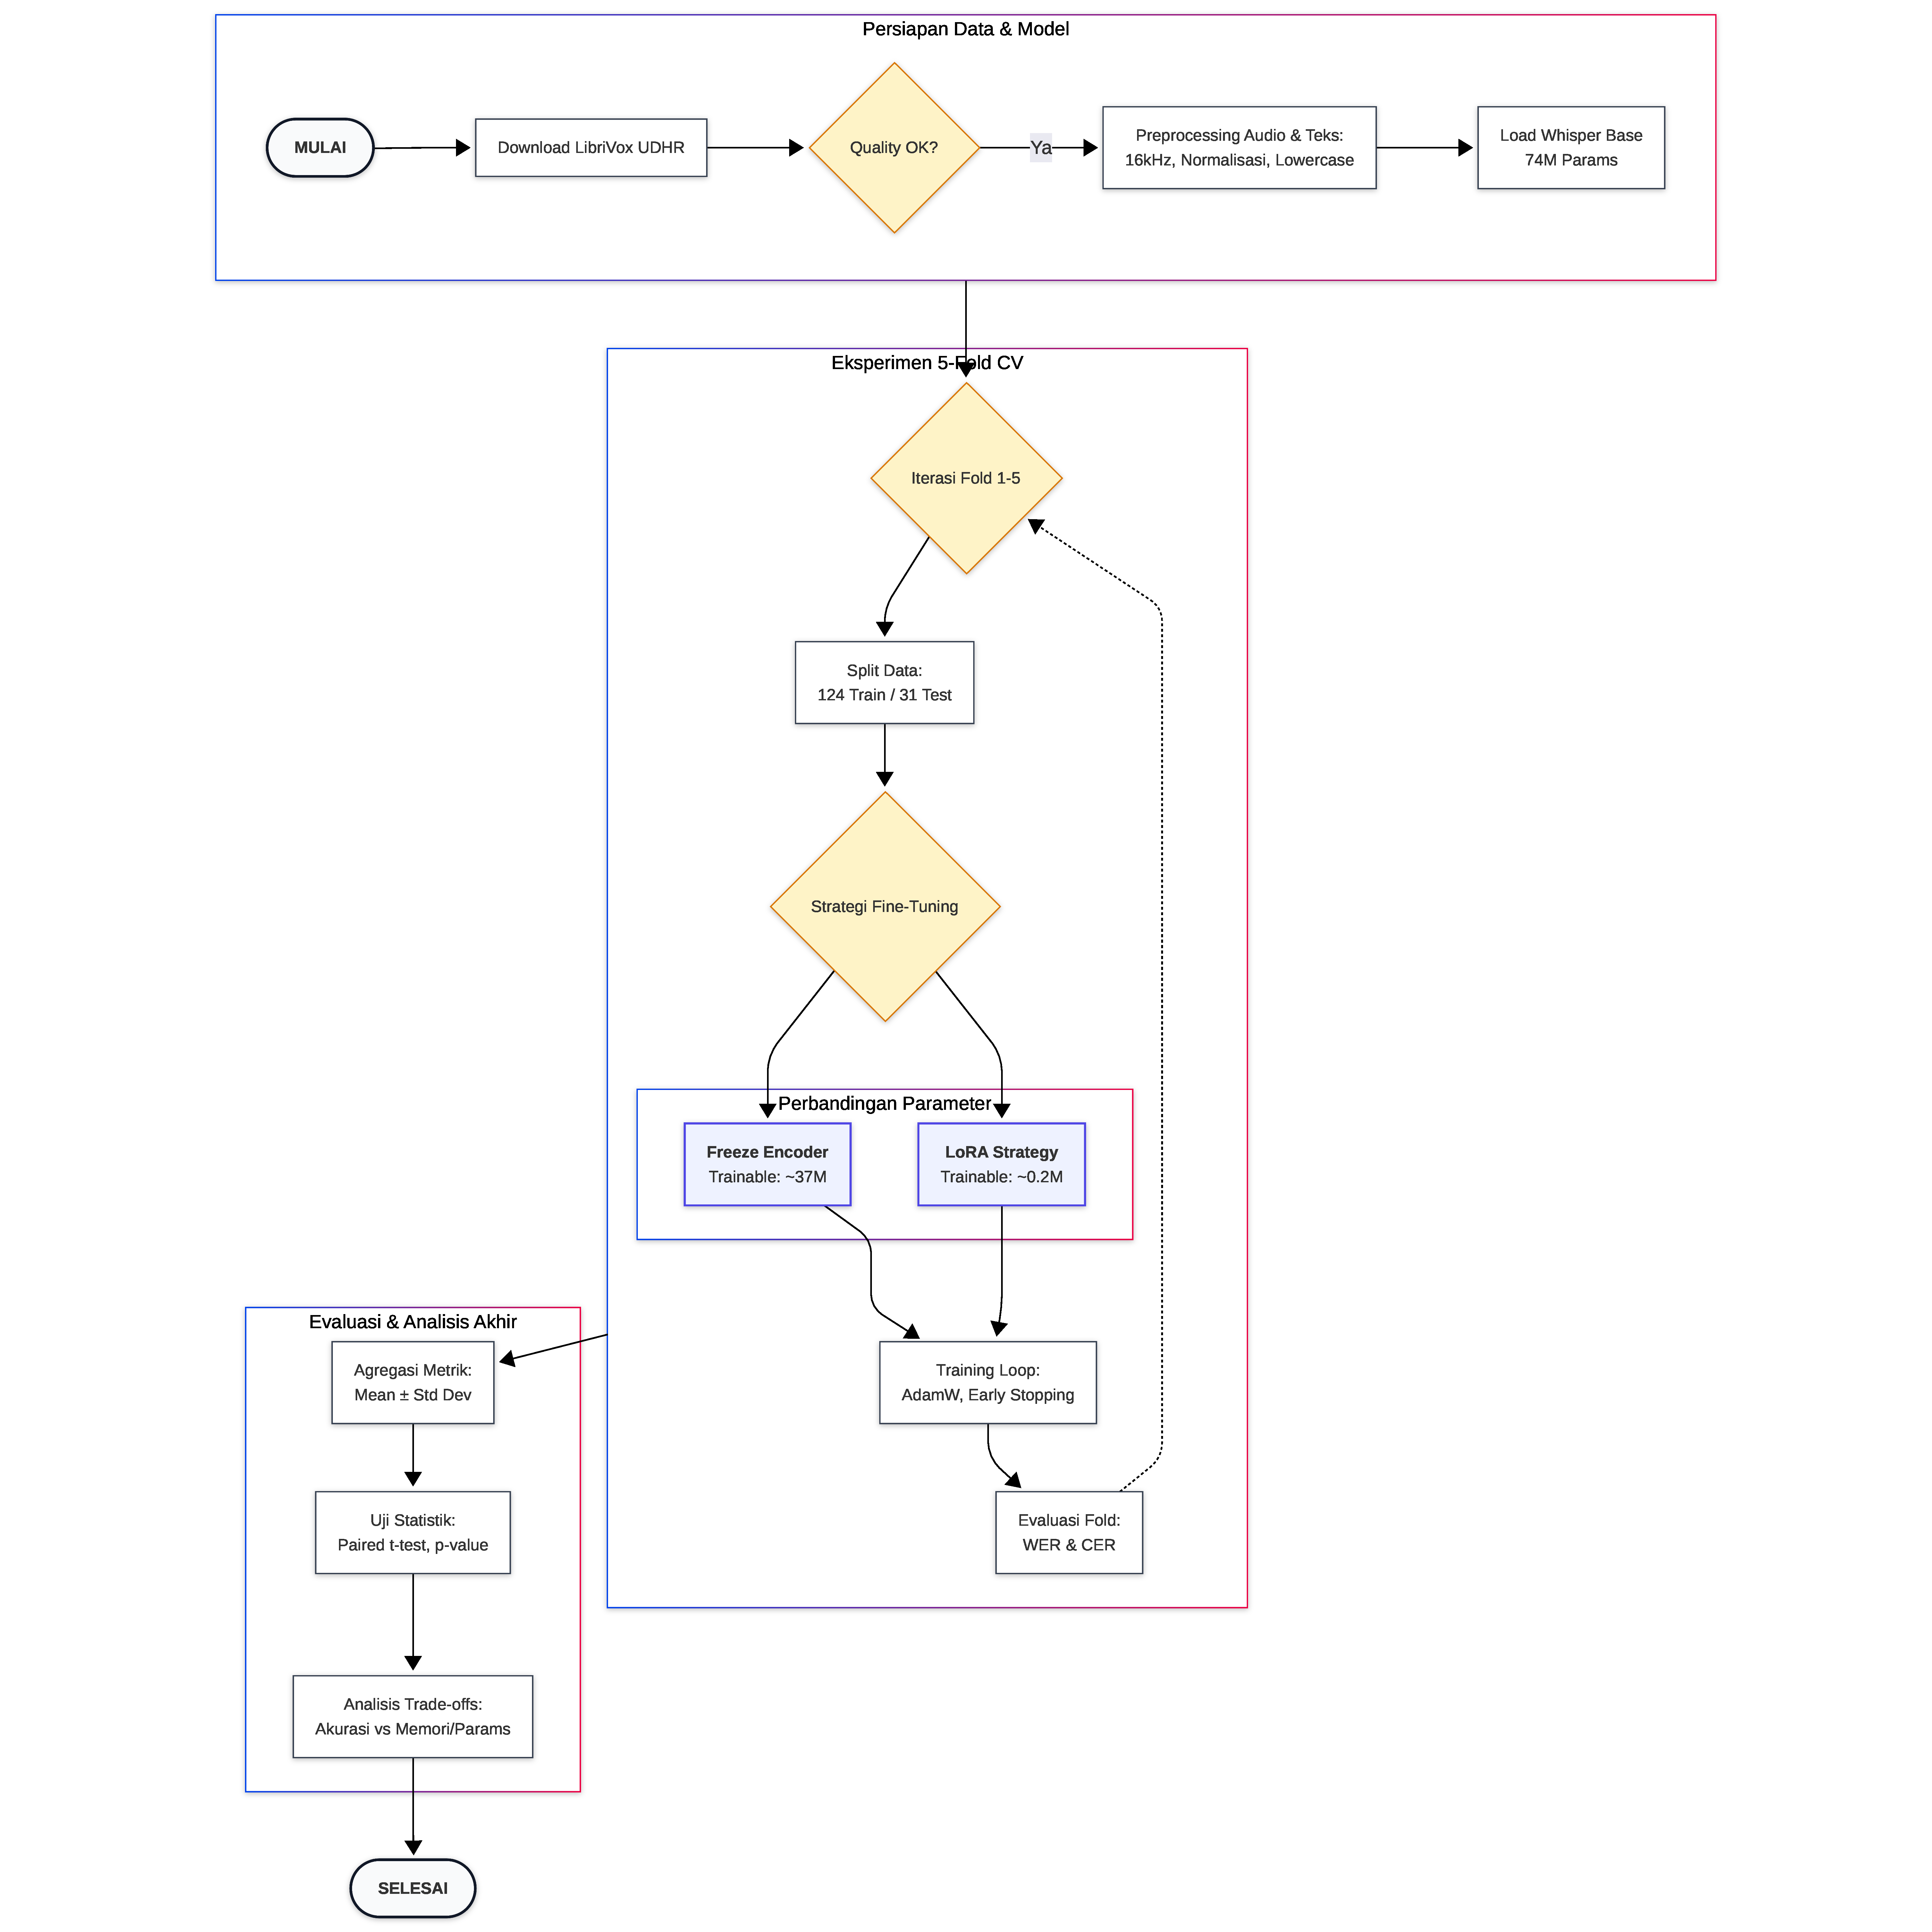
\includegraphics[width=0.8\textwidth]{figure/Development_Flow.pdf}
\caption{Alur Pengembangan Sistem}
\label{fig:3.alur_dev}
\end{figure}

\subsection{Metodologi Fine-Tuning}
\label{III.Metodologi_FT}

Metodologi fine-tuning mengikuti best practices untuk low-resource ASR:

\subsubsection{Full Fine-Tuning Methodology}

\begin{enumerate}[noitemsep]
    \item Initialize dari pre-trained Whisper Small checkpoint
    \item Freeze feature extractor (convolutional layers)
    \item Unfreeze encoder dan decoder Transformer blocks
    \item Training dengan supervised learning pada dataset Minangkabau
    \item Monitoring validation WER untuk early stopping
    \item Save best checkpoint berdasarkan validation performance
\end{enumerate}

\subsubsection{LoRA Fine-Tuning Methodology}

\begin{enumerate}[noitemsep]
    \item Initialize dari pre-trained Whisper Small checkpoint
    \item Freeze seluruh base model parameters
    \item Inject LoRA adapters pada Query dan Value projections
    \item Training hanya LoRA parameters ($\sim$2\% dari total)
    \item Monitoring validation WER untuk early stopping
    \item Merge LoRA weights dengan base model untuk inference
\end{enumerate}

\subsection{Metode Pengujian}
\label{III.Metode_Uji}

Pengujian dilakukan secara sistematis untuk memvalidasi performa model:

\subsubsection{Functional Testing}

\begin{enumerate}[noitemsep]
    \item \textbf{Audio Input Testing}: Verifikasi model dapat menerima berbagai format audio
    \item \textbf{Transcription Testing}: Verifikasi output transkrip dalam format text yang benar
    \item \textbf{Language Identification}: Verifikasi model mengenali bahasa Minangkabau dengan benar
    \item \textbf{Robustness Testing}: Test dengan audio berkualitas rendah, background noise
\end{enumerate}

\subsubsection{Performance Testing}

\begin{enumerate}[noitemsep]
    \item \textbf{Accuracy Testing}: Evaluasi WER dan CER pada test set
    \item \textbf{Inference Speed Testing}: Pengukuran Real-Time Factor (RTF)
    \item \textbf{Memory Usage Testing}: Monitoring GPU/CPU memory consumption
    \item \textbf{Scalability Testing}: Test dengan varying input lengths
\end{enumerate}

\subsubsection{Comparative Testing}

\begin{enumerate}[noitemsep]
    \item Perbandingan Base Whisper Small vs Fine-tuned models
    \item Perbandingan Full Fine-Tuning vs LoRA
    \item Statistical significance testing (paired t-test untuk WER/CER differences)
\end{enumerate}

\section{Ilustrasi Perhitungan Metode}
\label{III.Ilustrasi}

Bagian ini menjelaskan contoh perhitungan untuk metrik evaluasi utama yang digunakan dalam penelitian.

\subsection{Perhitungan Word Error Rate (WER)}
\label{III.Ilustrasi_WER}

WER mengukur edit distance pada level kata antara reference dan hypothesis transcription.

\subsubsection{Formula WER}

\vspace{0.3cm}
\begin{equation}
\label{eq:wer_def}
\text{WER} = \frac{S + D + I}{N} \times 100\%
\end{equation}
\myequations{Definisi WER (Word Error Rate)}
\vspace{0.2cm}

\noindent
di mana:
\begin{itemize}[noitemsep]
    \item $S$ = number of substitutions (kata salah diganti)
    \item $D$ = number of deletions (kata hilang)
    \item $I$ = number of insertions (kata tambahan)
    \item $N$ = total words dalam reference
\end{itemize}

\subsubsection{Contoh Perhitungan}

Misalkan kita memiliki pasangan reference-hypothesis berikut:

\textbf{Reference:} ``\textit{awak ingin pai ka pasar pagi iko}''

\textbf{Hypothesis:} ``\textit{awak ingin pergi pasar pagi ini}''

\textbf{Alignment:}
\begin{table}[H]
\centering
\begin{tabular}{|l|c|c|c|c|c|c|c|}
\hline
\textbf{Reference} & awak & ingin & pai & ka & pasar & pagi & iko \\
\hline
\textbf{Hypothesis} & awak & ingin & pergi & - & pasar & pagi & ini \\
\hline
\textbf{Operation} & C & C & S & D & C & C & S \\
\hline
\end{tabular}
\caption{Alignment untuk perhitungan WER (C=Correct, S=Substitution, D=Deletion)}
\end{table}

\textbf{Perhitungan:}
\begin{itemize}[noitemsep]
    \item Substitutions ($S$): 2 (``pai'' $\rightarrow$ ``pergi'', ``iko'' $\rightarrow$ ``ini'')
    \item Deletions ($D$): 1 (``ka'' dihapus)
    \item Insertions ($I$): 0
    \item Total words ($N$): 7
\end{itemize}

\vspace{0.3cm}
\begin{equation}
\label{eq:wer_example}
\text{WER} = \frac{2 + 1 + 0}{7} \times 100\% = \frac{3}{7} \times 100\% = 42.86\%
\end{equation}
\myequations{Contoh Perhitungan WER}
\vspace{0.2cm}

\subsection{Perhitungan Character Error Rate (CER)}
\label{III.Ilustrasi_CER}

CER mengukur edit distance pada level karakter, lebih sensitif terhadap phonetic errors.

\subsubsection{Formula CER}

\vspace{0.3cm}
\begin{equation}
\label{eq:cer_def}
\text{CER} = \frac{S_c + D_c + I_c}{N_c} \times 100\%
\end{equation}
\myequations{Definisi CER (Character Error Rate)}
\vspace{0.2cm}

\noindent
di mana:
\begin{itemize}[noitemsep]
    \item $S_c$ = number of character substitutions
    \item $D_c$ = number of character deletions
    \item $I_c$ = number of character insertions
    \item $N_c$ = total characters dalam reference
\end{itemize}

\subsubsection{Contoh Perhitungan}

Menggunakan contoh yang sama:

\textbf{Reference:} ``\textit{awakinginpaiakapasarpagiko}'' (tanpa spasi: 30 karakter)

\textbf{Hypothesis:} ``\textit{awakinginpergipasarpagini}'' (tanpa spasi: 28 karakter)

\textbf{Perhitungan:}
\begin{itemize}[noitemsep]
    \item Character substitutions ($S_c$): 5 (``p''→``p'', ``a''→``e'', ``i''→``r'', ``k''→``g'', ``o''→``i'')
    \item Character deletions ($D_c$): 2 (``k'', ``a'' dari kata ``ka'')
    \item Character insertions ($I_c$): 0
    \item Total characters ($N_c$): 30
\end{itemize}

\vspace{0.3cm}
\begin{equation}
\label{eq:cer_example}
\text{CER} = \frac{5 + 2 + 0}{30} \times 100\% = \frac{7}{30} \times 100\% = 23.33\%
\end{equation}
\myequations{Contoh Perhitungan CER}
\vspace{0.2cm}

\noindent
Perhatikan bahwa CER (23.33\%) lebih rendah dari WER (42.86\%) karena partial word matches dihargai pada level karakter.

\subsection{Perhitungan LoRA Parameters}
\label{III.Ilustrasi_LoRA}

Perhitungan jumlah trainable parameters untuk LoRA adaptation.

\subsubsection{Formula LoRA Parameters}

Untuk setiap attention layer dengan projection weight $W \in \mathbb{R}^{d \times k}$, LoRA menambahkan:

\vspace{0.3cm}
\begin{equation}
\label{eq:lora_params}
\text{LoRA params} = r \times (d + k)
\end{equation}
\myequations{Formula Parameter LoRA}
\vspace{0.2cm}

\noindent
di mana $r$ adalah rank.

\subsubsection{Contoh Perhitungan untuk Whisper Small}

Whisper Small memiliki:
\begin{itemize}[noitemsep]
    \item Total layers: 24 (12 encoder + 12 decoder)
    \item Hidden dimension ($d$): 768
    \item Projection dimension ($k$): 768
    \item LoRA rank ($r$): 8
    \item LoRA applied to: Query dan Value projections (2 per layer)
\end{itemize}

\textbf{Perhitungan per layer:}

\vspace{0.3cm}
\begin{equation}
\label{eq:lora_per_projection}
\text{Params per projection} = 8 \times (768 + 768) = 8 \times 1536 = 12,288
\end{equation}
\myequations{Parameter LoRA Per Projection}
\vspace{0.2cm}

\vspace{0.3cm}
\begin{equation}
\label{eq:lora_per_layer}
\text{Params per layer} = 2 \times 12,288 = 24,576
\end{equation}
\myequations{Parameter LoRA Per Layer}
\vspace{0.2cm}

\textbf{Total LoRA parameters:}

\vspace{0.3cm}
\begin{equation}
\label{eq:lora_total}
\text{Total LoRA params} = 24 \times 24,576 = 589,824 \approx 0.59\text{M}
\end{equation}
\myequations{Total Parameter LoRA}
\vspace{0.2cm}

\textbf{Percentage of total parameters:}

\vspace{0.3cm}
\begin{equation}
\label{eq:lora_percentage}
\text{Percentage} = \frac{589,824}{244,000,000} \times 100\% \approx 0.24\%
\end{equation}
\myequations{Persentase Parameter LoRA Terhadap Total}
\vspace{0.2cm}

\noindent
Ini menunjukkan bahwa LoRA hanya melatih $\sim$0.24\% dari total parameters Whisper Small, sangat efisien dibanding full fine-tuning.


    \newpage
\chapter{HASIL DAN PEMBAHASAN} \label{Bab IV}

\section{Pendahuluan}

Bab ini menyajikan hasil eksperimen \textit{fine-tuning} model Whisper Base pada bahasa Minangkabau menggunakan dua strategi: \textit{Freeze Encoder} dan \textit{Low-Rank Adaptation} (LoRA) \cite{hu2022lora}. Kedua strategi dievaluasi menggunakan metodologi 5-\textit{fold cross-validation} \cite{kohavi1995crossvalidation} pada dataset yang sama (156 file audio, $\sim$1,3 jam) untuk memastikan perbandingan yang adil. Bab ini dimulai dengan hasil masing-masing strategi, dilanjutkan dengan analisis perbandingan dan pembahasan.

%% ====================================================================
%% SECTION: HASIL FREEZE ENCODER
%% ====================================================================
\section{Hasil Strategi Freeze Encoder} \label{IV.FreezeEncoder}

\subsection{Perbandingan Eksperimen Freeze Encoder}

Selama proses penelitian, dilakukan lima kali percobaan pelatihan (\textit{run}) dengan strategi \textit{Freeze Encoder} untuk menemukan konfigurasi optimal. Tabel~\ref{tab:fe_run_configs} merangkum konfigurasi yang digunakan pada setiap percobaan, dan Tabel~\ref{tab:fe_run_comparison} merangkum hasilnya.

\begin{table}[H]
\centering
\caption{Konfigurasi Hyperparameter Lima Percobaan Freeze Encoder}
\label{tab:fe_run_configs}
\resizebox{\textwidth}{!}{%
\begin{tabular}{|l|c|c|c|c|c|}
\hline
\textbf{Parameter} & \textbf{Run 1} & \textbf{Run 2} & \textbf{Run 3} & \textbf{Run 4} & \textbf{Run 5} \\
 & \textbf{(22 Jan, 16:00)} & \textbf{(22 Jan, 16:57)} & \textbf{(22 Jan, 17:32)} & \textbf{(8 Feb, 14:51)} & \textbf{(12 Feb, 06:00)} \\
\hline
\hline
\multicolumn{6}{|c|}{\textbf{Konfigurasi Training}} \\
\hline
Learning Rate & 5$\times$10\textsuperscript{-6} & 1$\times$10\textsuperscript{-5} & 1$\times$10\textsuperscript{-5} & 1$\times$10\textsuperscript{-5} & 1$\times$10\textsuperscript{-5} \\
\hline
Batch Size & 16 & 16 & 16 & 32 & 32 \\
\hline
Gradient Accumulation & 2 & 2 & 2 & 1 & 1 \\
\hline
Effective Batch Size & 32 & 32 & 32 & 32 & 32 \\
\hline
Max Steps & 200 & 200 & 200 & 200 & 120 \\
\hline
Warmup Ratio & 0,2 & 0,2 & 0,2 & 0,2 & 0,2 \\
\hline
Weight Decay & 0,2 & 0,2 & 0,2 & 0,1 & 0,1 \\
\hline
Label Smoothing & --- & --- & --- & --- & 0,1 \\
\hline
LR Scheduler & Cosine & Cosine & Cosine & Cosine & Cosine \\
\hline
\hline
\multicolumn{6}{|c|}{\textbf{Konfigurasi Dropout Model}} \\
\hline
Decoder Dropout & 0,3 & 0,3 & 0,3 & 0,3 & 0,2 \\
\hline
Attention Dropout & 0,2 & 0,2 & 0,2 & 0,2 & 0,15 \\
\hline
Activation Dropout & 0,2 & 0,2 & 0,2 & 0,2 & 0,15 \\
\hline
\hline
\multicolumn{6}{|c|}{\textbf{Decoding}} \\
\hline
Beam Width & 1 (greedy) & 1 (greedy) & 1 (greedy) & 5 & 5 \\
\hline
\end{tabular}%
}
\end{table}

\begin{table}[H]
\centering
\caption{Perbandingan Hasil Lima Percobaan Freeze Encoder}
\label{tab:fe_run_comparison}
\resizebox{\textwidth}{!}{%
\begin{tabular}{|c|c|c|c|c|c|c|c|}
\hline
\textbf{Run} & \textbf{Learning Rate} & \textbf{Batch Size} & \textbf{Weight Decay} & \textbf{Label Smooth.} & \textbf{Beam} & \textbf{Mean WER (\%)} & \textbf{Mean CER (\%)} \\
\hline
1 (22 Jan, 16:00) & 5$\times$10\textsuperscript{-6} & 16$\times$2 & 0,2 & --- & 1 & 25,07 $\pm$ 2,86 & 5,60 $\pm$ 0,59 \\
\hline
2 (22 Jan, 16:57) & 1$\times$10\textsuperscript{-5} & 16$\times$2 & 0,2 & --- & 1 & 22,34 $\pm$ 1,89 & 4,93 $\pm$ 0,55 \\
\hline
3 (22 Jan, 17:32) & 1$\times$10\textsuperscript{-5} & 16$\times$2 & 0,2 & --- & 1 & 22,95 $\pm$ 2,70 & 5,52 $\pm$ 0,77 \\
\hline
4 (8 Feb, 14:51) & 1$\times$10\textsuperscript{-5} & 32$\times$1 & 0,1 & --- & 5 & 19,92 $\pm$ 2,42 & 4,53 $\pm$ 0,65 \\
\hline
\textbf{5 (12 Feb, 06:00)} & \textbf{1$\times$10\textsuperscript{-5}} & \textbf{32$\times$1} & \textbf{0,1} & \textbf{0,1} & \textbf{5} & \textbf{20,34 $\pm$ 2,41} & \textbf{4,46 $\pm$ 0,50} \\
\hline
\end{tabular}%
}
\end{table}

Run 5 mencapai performa terbaik dengan rata-rata WER \textbf{20,34\%} dan CER \textbf{4,46\%}. Meskipun WER rata-rata Run 5 sedikit lebih tinggi dibandingkan Run 4 (20,34\% vs 19,92\%), Run 5 mencapai CER yang lebih rendah (4,46\% vs 4,53\%) dan standar deviasi WER yang lebih kecil (2,41\% vs 2,42\%). Berdasarkan analisis konfigurasi pada Tabel~\ref{tab:fe_run_configs}, evolusi percobaan menunjukkan beberapa temuan:

\begin{enumerate}
    \item \textbf{Run 1 vs Run 2} (pengaruh \textit{learning rate}): Peningkatan \textit{learning rate} dari 5$\times$10\textsuperscript{-6} ke 1$\times$10\textsuperscript{-5} menghasilkan penurunan WER signifikan (25,07\% $\rightarrow$ 22,34\%), menunjukkan bahwa \textit{learning rate} awal terlalu kecil untuk konvergensi yang efektif.
    
    \item \textbf{Run 2 vs Run 3} (reproduktibilitas): Kedua run menggunakan konfigurasi identik namun menghasilkan WER yang berbeda (22,34\% vs 22,95\%), menunjukkan variabilitas dari \textit{stochastic training} yang perlu diperhatikan dalam interpretasi hasil.
    
    \item \textbf{Run 4} (optimasi multi-faktor): Penurunan \textit{weight decay} dari 0,2 ke 0,1, peningkatan \textit{batch size} fisik dari 16 menjadi 32, dan penggunaan \textit{beam search} (\textit{width}=5) menghasilkan penurunan WER signifikan (22,34\% $\rightarrow$ 19,92\%) \cite{radford2023whisper}.
    
    \item \textbf{Run 5} (\textit{label smoothing} + penyesuaian regularisasi): Penambahan \textit{label smoothing} 0,1 \cite{szegedy2016rethinking} dengan penurunan \textit{dropout} (0,2/0,15/0,15 vs 0,3/0,2/0,2 pada Run 4) dan pengurangan \textit{max steps} (120 vs 200) menghasilkan model dengan CER lebih rendah (4,46\% vs 4,53\%) dan konsistensi yang lebih baik (std WER 2,41\% vs 2,42\%). \textit{Label smoothing} membagi beban regularisasi dengan \textit{dropout}, sehingga \textit{dropout} dapat diturunkan tanpa meningkatkan risiko \textit{overfitting}.
\end{enumerate}

Analisis selanjutnya menggunakan hasil dari \textbf{Run 5} (run\_20260212\_060037) karena menggunakan konfigurasi regularisasi terlengkap dan menunjukkan keseimbangan terbaik antara performa dan konsistensi.

\subsection{Hasil Cross-Validation Freeze Encoder}

Tabel~\ref{tab:fe_cv_results} menunjukkan hasil evaluasi 5-\textit{fold cross-validation} untuk strategi \textit{Freeze Encoder}.

\begin{table}[H]
\centering
\caption{Hasil 5-Fold Cross-Validation Strategi Freeze Encoder}
\label{tab:fe_cv_results}
\begin{tabular}{|c|c|c|c|c|c|}
\hline
\textbf{Fold} & \textbf{Train} & \textbf{Eval} & \textbf{WER (\%)} & \textbf{CER (\%)} & \textbf{Steps} \\
\hline
0 & 124 & 32 & 20,36 & 4,28 & 96 \\
\hline
1 & 125 & 31 & 19,76 & 4,58 & 116 \\
\hline
2 & 125 & 31 & \textbf{16,81} & \textbf{3,60} & 108 \\
\hline
3 & 125 & 31 & 24,37 & 4,90 & 120 \\
\hline
4 & 125 & 31 & 20,41 & 4,96 & 116 \\
\hline
\hline
\textbf{Mean} & \textbf{125} & \textbf{31} & \textbf{20,34 $\pm$ 2,41} & \textbf{4,46 $\pm$ 0,50} & \textbf{111,2} \\
\hline
\end{tabular}
\end{table}

\textbf{Catatan Metodologi}: \textit{Evaluation set} juga digunakan untuk \textit{early stopping} selama training (setiap 4 steps). Pendekatan ini merupakan \textit{pragmatic trade-off} yang umum dalam riset \textit{extremely low-resource}, di mana memisahkan \textit{validation set} akan mengurangi data training secara signifikan. Metrik yang dilaporkan berasal dari \textit{best checkpoint} dan berpotensi sedikit optimistis. Catatan metodologi ini berlaku juga untuk strategi LoRA.

\textit{Fold}~2 mencapai performa terbaik (WER 16,81\%, CER 3,60\%), sedangkan \textit{Fold}~3 menunjukkan WER tertinggi (24,37\%). Rentang WER antar-\textit{fold} sebesar 7,56 poin persentase mencerminkan sensitivitas model terhadap pembagian data pada dataset kecil.

\subsection{Konvergensi Training Freeze Encoder}

Gambar~\ref{fig:fe_training_loss} menampilkan kurva \textit{training loss} untuk kelima \textit{fold} pada strategi \textit{Freeze Encoder}.

\begin{figure}[H]
\centering
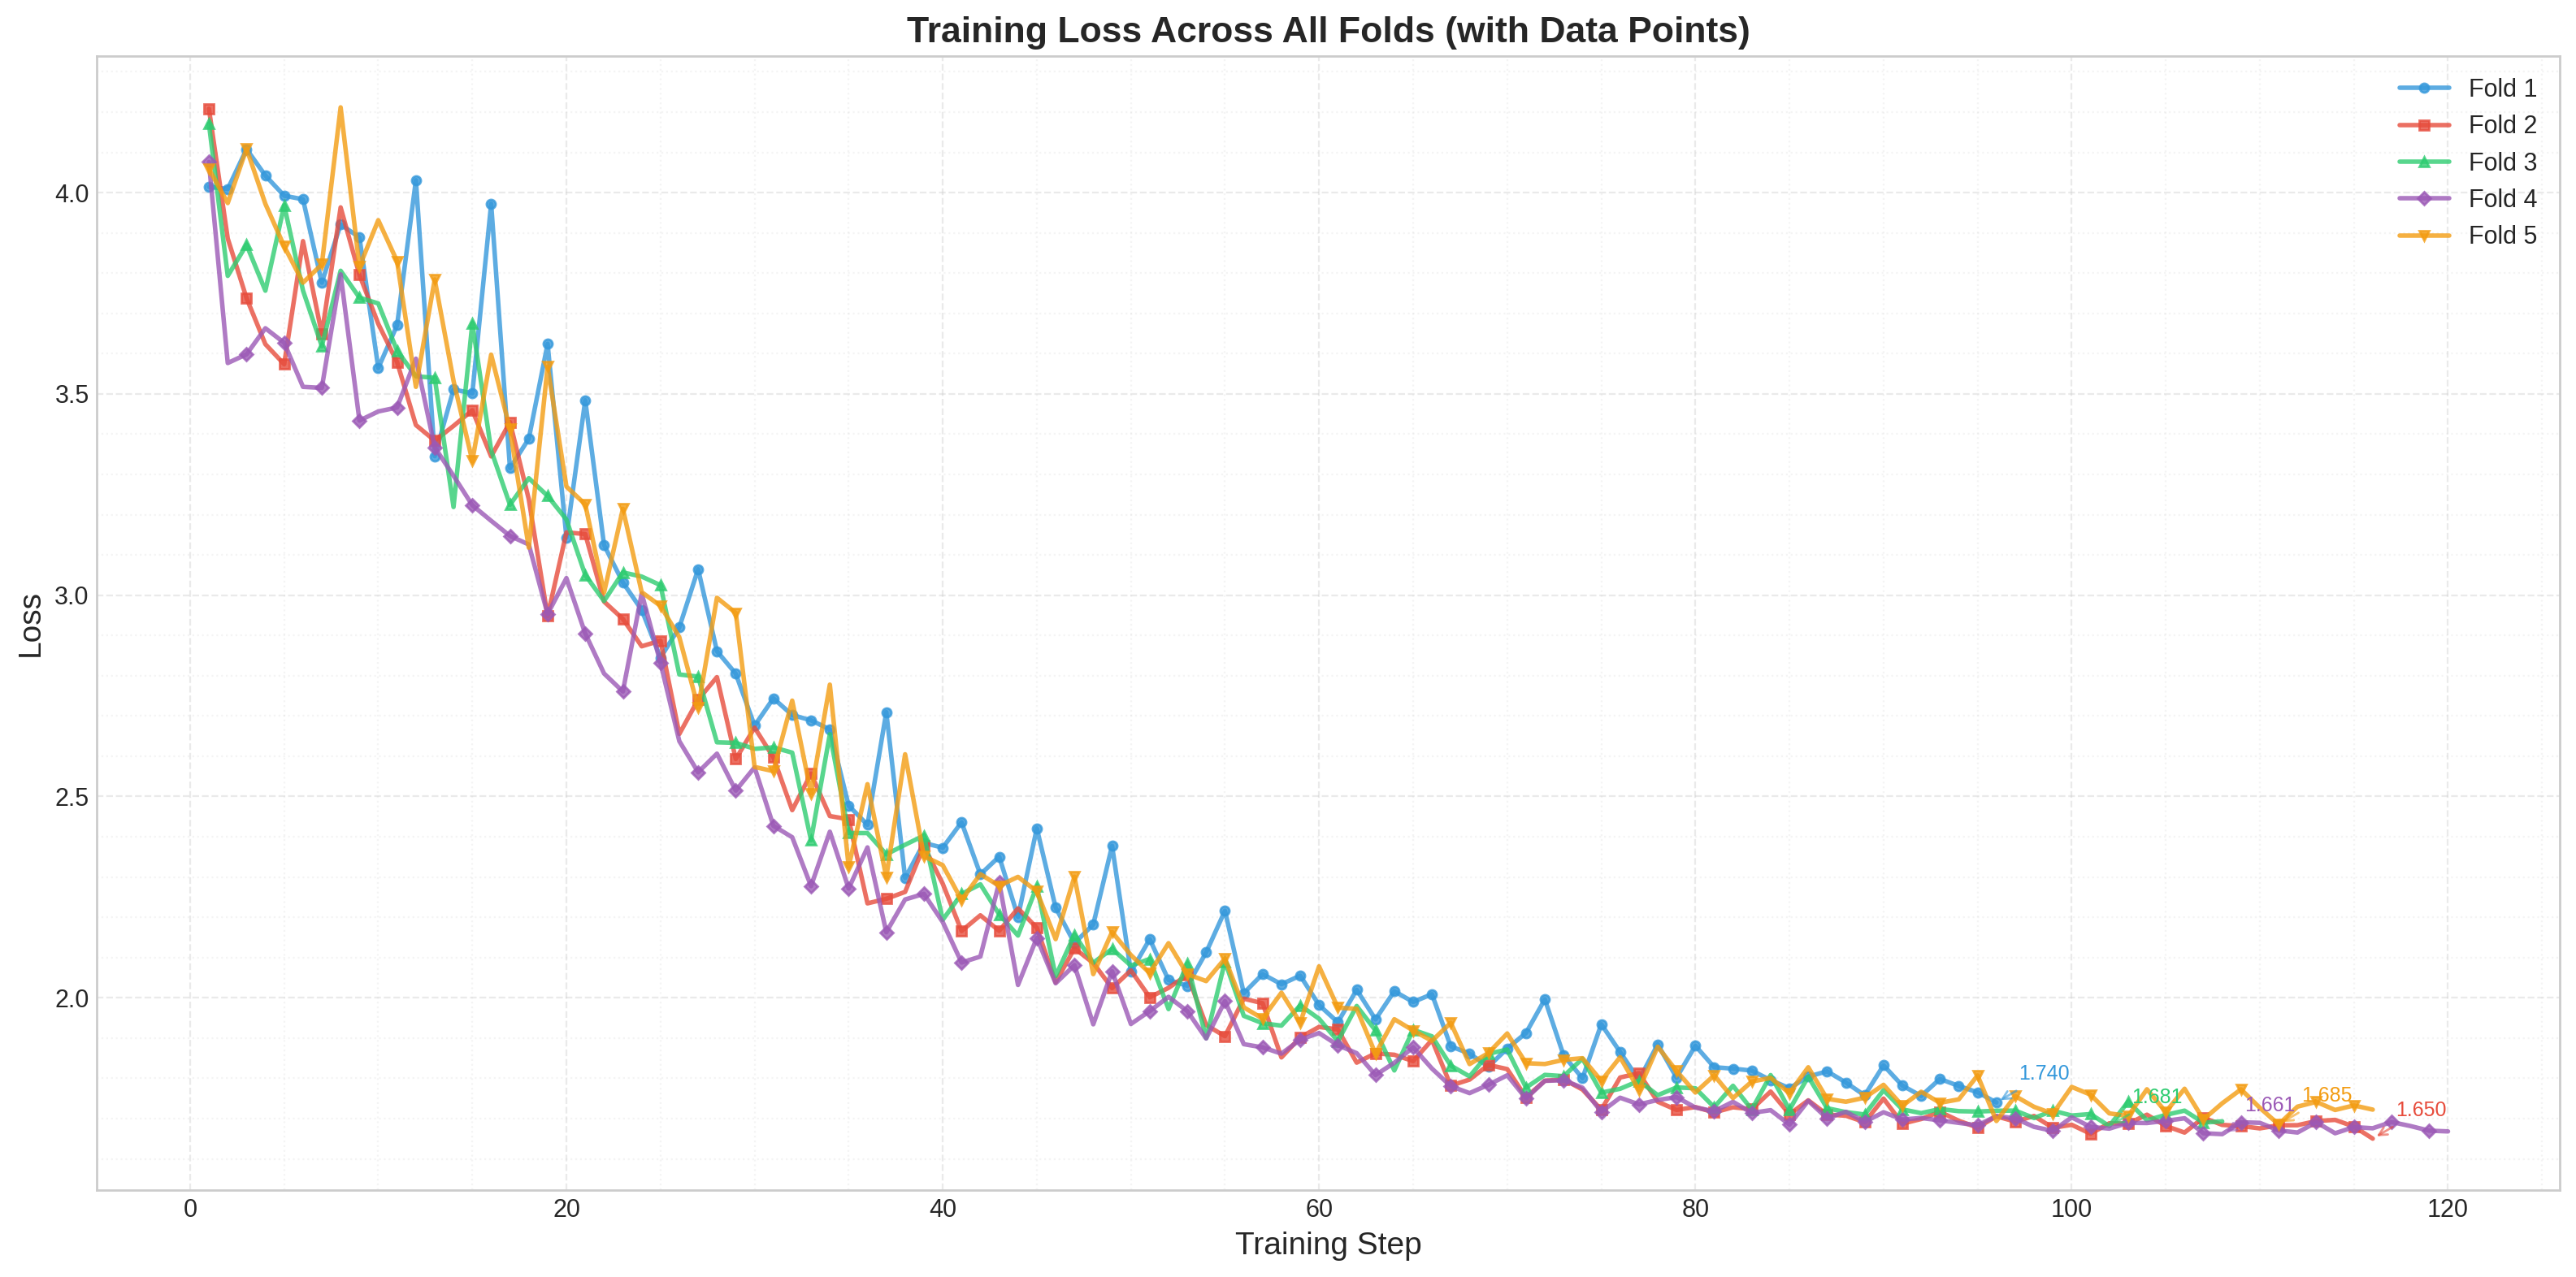
\includegraphics[width=0.8\textwidth]{code/freeze_encoder/outputs/metrics/run_20260212_060037/visualizations/training_loss_detailed.png}
\caption{Kurva Training Loss --- Strategi Freeze Encoder}
\label{fig:fe_training_loss}
\end{figure}

Tabel~\ref{tab:fe_training_summary} merangkum statistik training untuk setiap \textit{fold}:

\begin{table}[H]
\centering
\caption{Ringkasan Training Freeze Encoder per Fold}
\label{tab:fe_training_summary}
\begin{tabular}{|c|c|c|c|c|}
\hline
\textbf{Fold} & \textbf{Steps} & \textbf{Initial Loss} & \textbf{Final Loss} & \textbf{Epoch} \\
\hline
0 & 96 & 4,014 & 1,740 & 24 \\
\hline
1 & 116 & 4,208 & 1,650 & 29 \\
\hline
2 & 108 & 4,171 & 1,693 & 27 \\
\hline
3 & 120 & 4,076 & 1,668 & 30 \\
\hline
4 & 116 & 4,059 & 1,722 & 29 \\
\hline
\hline
\textbf{Mean} & \textbf{111,2} & \textbf{4,106} & \textbf{1,695} & \textbf{27,8} \\
\hline
\end{tabular}
\end{table}

Seluruh \textit{fold} berhasil menurunkan \textit{training loss} dari kisaran 4,0--4,2 menjadi $\sim$1,7. Tidak seperti Run 1--4 sebelumnya yang tanpa \textit{label smoothing} di mana loss menurun hingga $\sim$0,01, Run 5 menggunakan \textit{label smoothing factor} 0,1 yang secara sengaja mendistribusikan probabilitas ke seluruh \textit{vocabulary}, sehingga loss minimum teoritis bukan 0 melainkan $\sim$1,5 \cite{szegedy2016rethinking}. Hal ini mencegah model menjadi terlalu percaya diri (\textit{overconfident}) dan berfungsi sebagai regularisasi tambahan. \textit{Early stopping} (\textit{patience}=6 steps) berhasil menghentikan training sebelum batas 120 steps pada semua \textit{fold}.

\subsection{Metrik Evaluasi Freeze Encoder}

Gambar~\ref{fig:fe_eval_metrics} menunjukkan perkembangan WER dan CER selama evaluasi pada strategi \textit{Freeze Encoder}.

\begin{figure}[H]
\centering
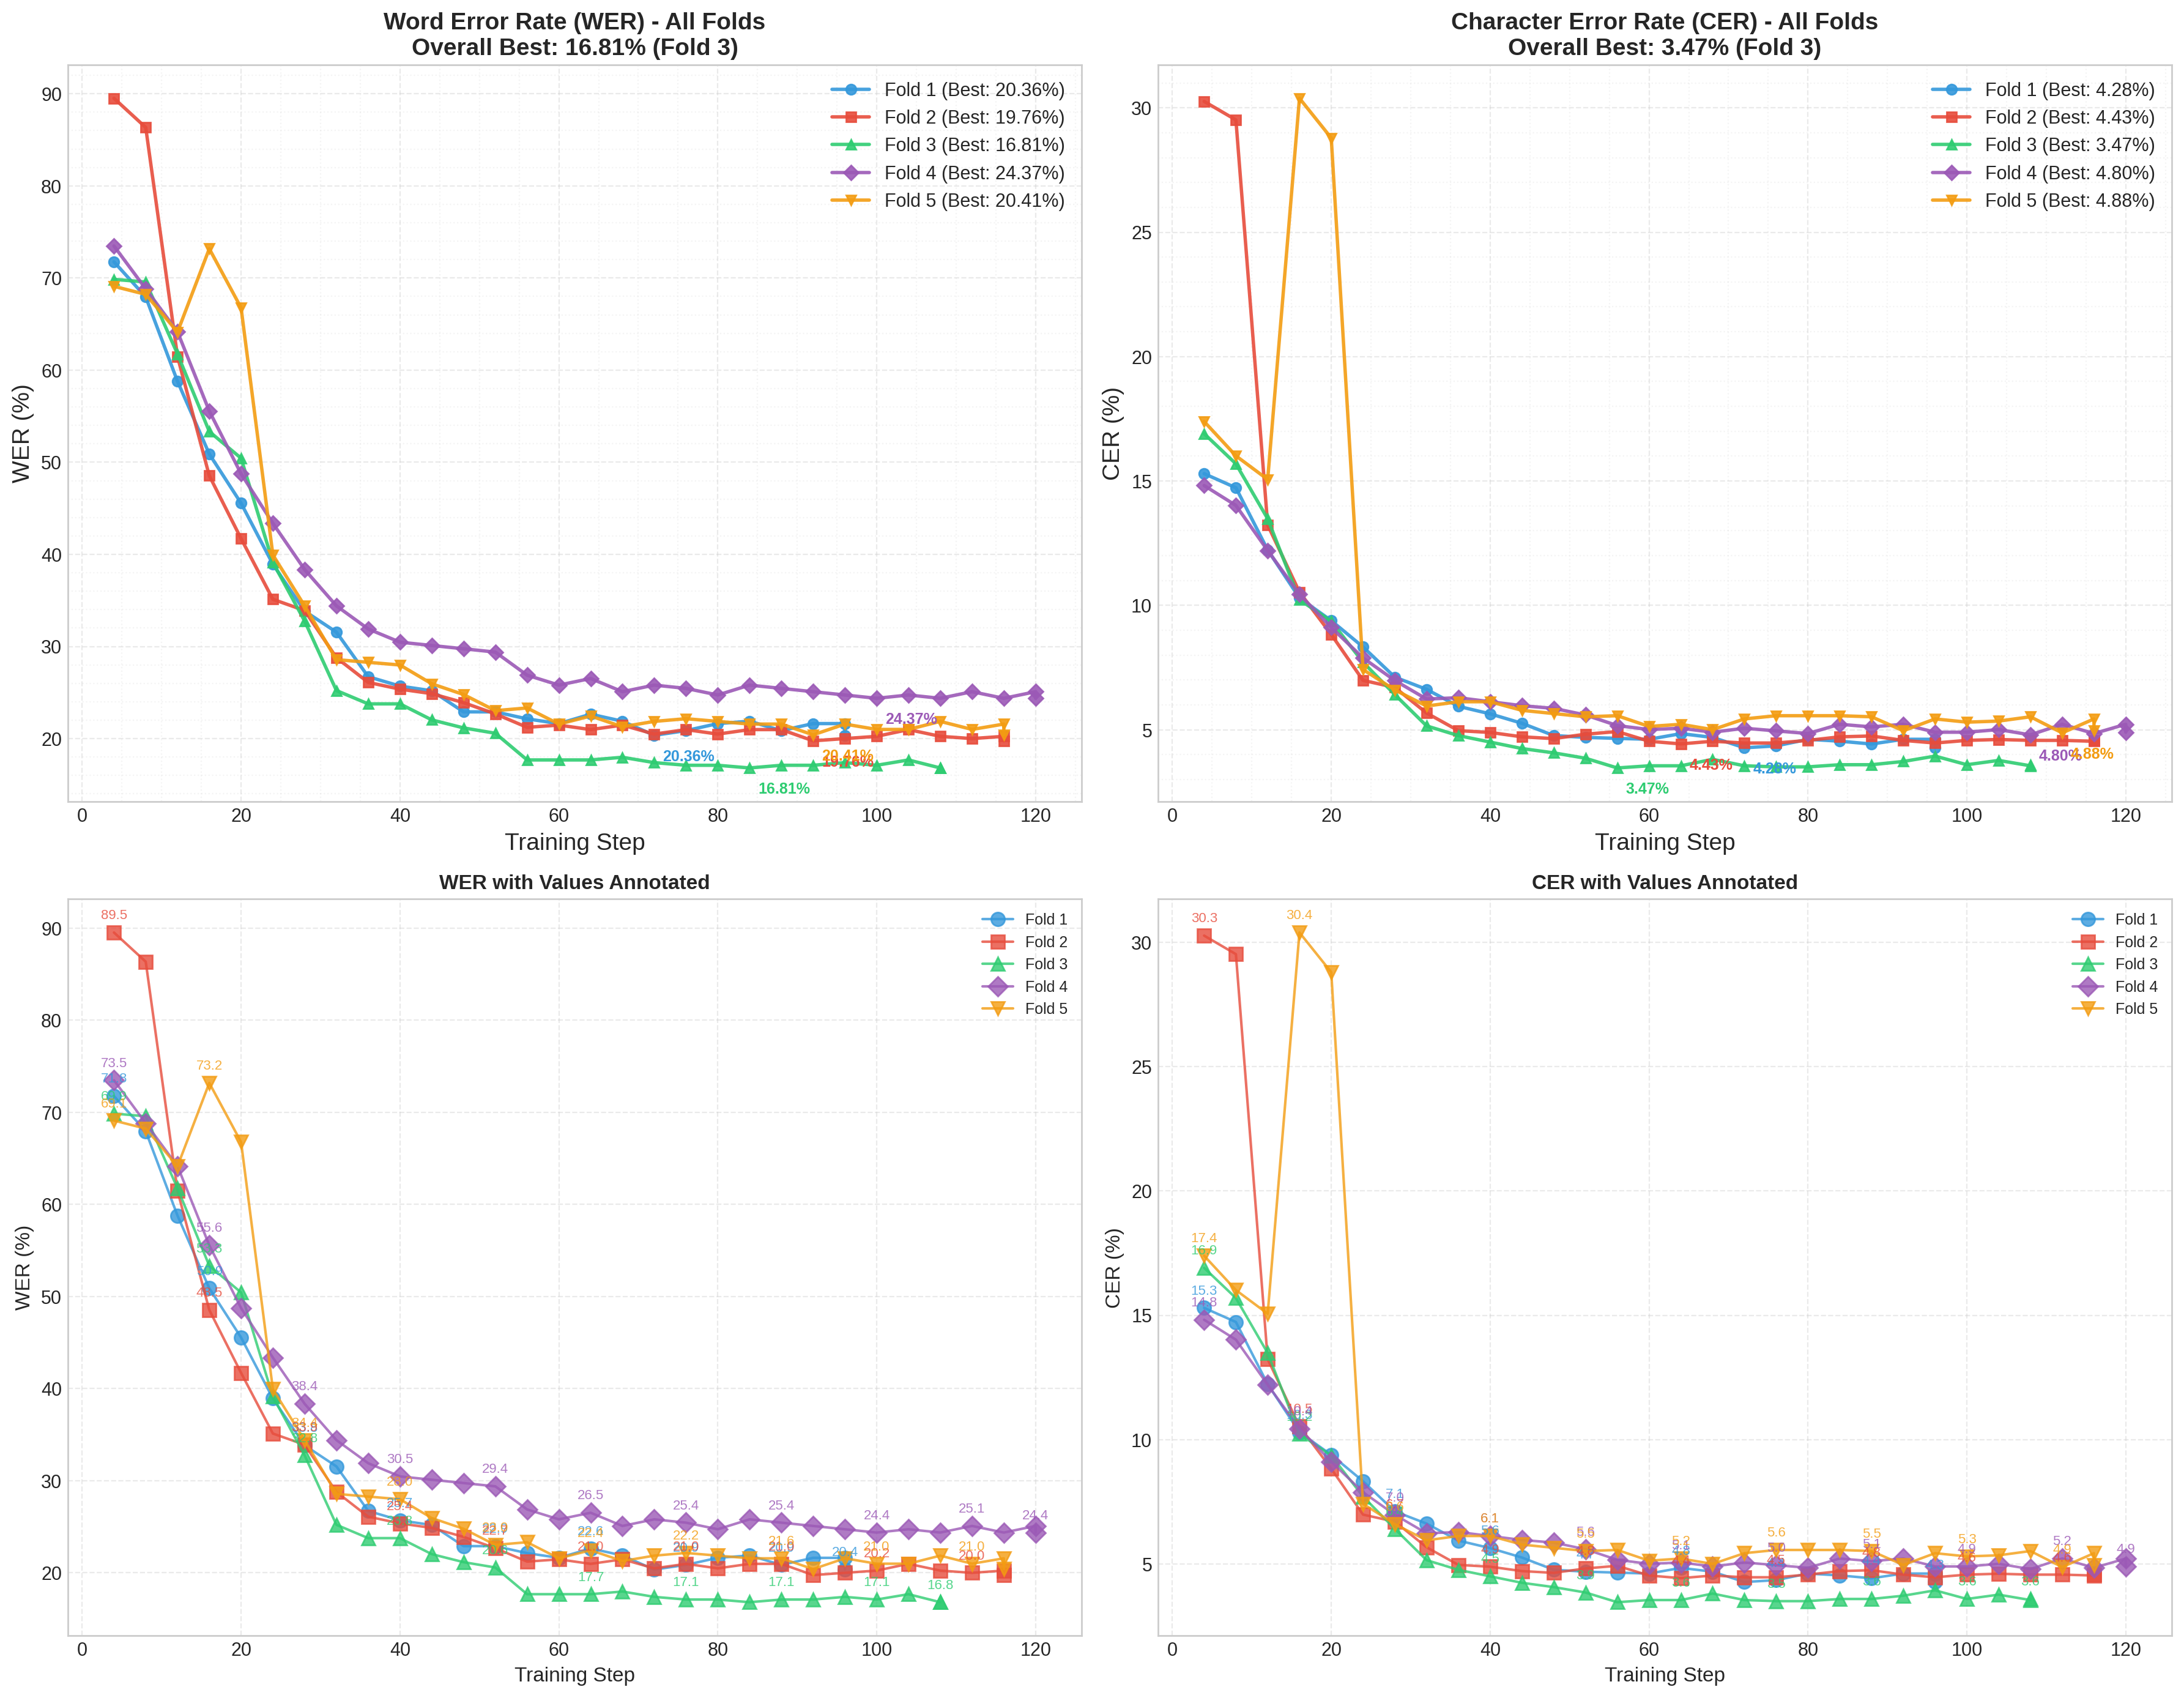
\includegraphics[width=0.9\textwidth]{code/freeze_encoder/outputs/metrics/run_20260212_060037/visualizations/evaluation_metrics_detailed.png}
\caption{Perkembangan WER dan CER --- Strategi Freeze Encoder}
\label{fig:fe_eval_metrics}
\end{figure}

Semua \textit{fold} menunjukkan penurunan WER yang signifikan dari rentang 70--73\% pada evaluasi awal menjadi 16--24\% pada evaluasi akhir. Beberapa pola penting yang teramati:

\begin{itemize}
    \item \textbf{Penurunan WER yang Cepat}: Sebagian besar penurunan WER terjadi pada 40--60 \textit{steps} pertama ($\sim$10--15 \textit{epochs}), di mana WER turun dari $>$70\% menjadi $\sim$25--30\%. Setelah itu, penurunan berlangsung lebih lambat dan bertahap menuju nilai konvergen.
    
    \item \textbf{Variasi Antar-Fold yang Tinggi}: Terdapat perbedaan yang cukup besar antar-\textit{fold} pada fase akhir training. \textit{Fold}~2 mencapai WER terendah (16,81\%) sementara \textit{Fold}~3 hanya mencapai 24,37\%, dengan rentang 7,56 poin persentase. Variasi ini mengindikasikan sensitivitas tinggi terhadap komposisi data training dan evaluasi pada dataset kecil.
    
    \item \textbf{CER Lebih Stabil}: Dibandingkan WER, kurva CER menunjukkan konvergensi yang lebih seragam antar-\textit{fold} dengan rentang akhir yang lebih sempit (3,60\%--4,96\%), menunjukkan bahwa kesalahan karakter lebih konsisten meskipun kesalahan kata bervariasi.
    
    \item \textbf{Fluktuasi pada Beberapa Fold}: Beberapa \textit{fold} menunjukkan fluktuasi metrik evaluasi pada fase pertengahan training, yang mengindikasikan ketidakstabilan optimasi akibat dataset yang sangat kecil dan jumlah parameter trainable yang besar (37M, 50\% dari total).
\end{itemize}

\subsection{Prediksi Model Freeze Encoder}

Tabel~\ref{tab:fe_predictions_fold2} menampilkan contoh prediksi pada \textit{Fold}~2 (fold terbaik, WER 16,81\%):

\begin{table}[H]
\centering
\caption{Contoh Prediksi Freeze Encoder pada Fold 2 (Fold Terbaik)}
\label{tab:fe_predictions_fold2}
\resizebox{\textwidth}{!}{%
\begin{tabular}{|p{0.42\textwidth}|p{0.42\textwidth}|c|c|}
\hline
\textbf{Referensi} & \textbf{Prediksi Model} & \textbf{WER} & \textbf{CER} \\
\hline
manusia sadonyo lahia ka dunia mambao hak hak dan kamardekaan mandasar nan samo dan indak dapek dipisahkan & 
manusia sadonyonyo lahia kadunian mambuh hak hak dan kamardekaan mandasar nan samo dan indak dapek dipisahkan & 
23,5\% & 5,7\% \\
\hline
sasungguahnyo ikrar negara negara anggota & 
susungguahnyo iklar negara negara anggota & 
40,0\% & 6,7\% \\
\hline
untuak mamajukan panghormatan taradok hak hak asasi manusia dan kamardekaan nan mandasar & 
untuak mamajukan pangormatan taradok hak hak asasi manusia dan kamardekaan nan mandasar & 
\textbf{8,3\%} & \textbf{1,1\%} \\
\hline
\end{tabular}%
}
\end{table}

Pola kesalahan utama pada \textit{Freeze Encoder} meliputi: (1) substitusi fonetik pada konsonan serupa (``deklarasi'' $\rightarrow$ ``rekelerasi'', ``sasungguahnyo'' $\rightarrow$ ``susungguahnyo''); (2) kesalahan segmentasi kata (``di antaro'' $\rightarrow$ ``diantaro'', ``anggota alah'' $\rightarrow$ ``anggotaalah''); dan (3) variasi partikel Minangkabau (``mampatahankannyo'' $\rightarrow$ ``mampatahankan jo'').

%% ====================================================================
%% SECTION: HASIL LoRA
%% ====================================================================
\section{Hasil Strategi LoRA} \label{IV.LoRA}

\subsection{Perbandingan Eksperimen LoRA}

Serupa dengan strategi \textit{Freeze Encoder}, dilakukan lima kali percobaan pelatihan (\textit{run}) dengan strategi LoRA untuk menemukan konfigurasi optimal. Setiap percobaan menggunakan variasi \textit{hyperparameter} yang berbeda, termasuk variasi \textit{rank}, \textit{learning rate}, \textit{weight decay}, dan \textit{dropout}. Tabel~\ref{tab:lora_run_configs} merangkum konfigurasi yang digunakan pada setiap percobaan.

\begin{table}[H]
\centering
\caption{Konfigurasi Hyperparameter Lima Percobaan LoRA}
\label{tab:lora_run_configs}
\resizebox{\textwidth}{!}{%
\begin{tabular}{|l|c|c|c|c|c|}
\hline
\textbf{Parameter} & \textbf{Run 1} & \textbf{Run 2} & \textbf{Run 3} & \textbf{Run 4} & \textbf{Run 5} \\
 & \textbf{(8 Feb, 16:30)} & \textbf{(8 Feb, 17:44)} & \textbf{(8 Feb, 18:51)} & \textbf{(8 Feb, 19:41)} & \textbf{(12 Feb, 06:32)} \\
\hline
\hline
\multicolumn{6}{|c|}{\textbf{Konfigurasi LoRA Adapter}} \\
\hline
Rank ($r$) & 8 & 8 & 16 & 8 & 8 \\
\hline
Alpha ($\alpha$) & 16 & 16 & 32 & 16 & 16 \\
\hline
Scaling ($\alpha / r$) & 2,0$\times$ & 2,0$\times$ & 2,0$\times$ & 2,0$\times$ & 2,0$\times$ \\
\hline
LoRA Dropout & 0,1 & 0,1 & 0,15 & 0,15 & 0,15 \\
\hline
Target Modules & \multicolumn{5}{c|}{q\_proj, v\_proj, k\_proj, out\_proj, fc1, fc2} \\
\hline
\hline
\multicolumn{6}{|c|}{\textbf{Konfigurasi Training}} \\
\hline
Learning Rate & 5$\times$10\textsuperscript{-4} & 5$\times$10\textsuperscript{-4} & 3$\times$10\textsuperscript{-4} & 7$\times$10\textsuperscript{-4} & 7$\times$10\textsuperscript{-4} \\
\hline
Batch Size & 32 & 32 & 32 & 32 & 32 \\
\hline
Max Steps & 400 & 400 & 250 & 250 & 200 \\
\hline
Warmup Ratio & 0,1 & 0,1 & 0,15 & 0,1 & 0,1 \\
\hline
Weight Decay & 0,01 & 0,01 & 0,03 & 0,05 & 0,05 \\
\hline
Label Smoothing & 0,1 & 0,1 & 0,05 & 0,1 & 0,1 \\
\hline
\hline
\multicolumn{6}{|c|}{\textbf{Konfigurasi Dropout Model}} \\
\hline
Decoder Dropout & 0,1 & 0,1 & 0,15 & 0,1 & 0,1 \\
\hline
Attention Dropout & 0,05 & 0,05 & 0,1 & 0,05 & 0,05 \\
\hline
Activation Dropout & 0,05 & 0,05 & 0,1 & 0,05 & 0,05 \\
\hline
\hline
\multicolumn{6}{|c|}{\textbf{Decoding}} \\
\hline
Beam Width & 5 & 5 & 5 & 5 & 5 \\
\hline
\end{tabular}%
}
\end{table}

Tabel~\ref{tab:lora_run_comparison} merangkum hasil performa dari seluruh percobaan LoRA.

\begin{table}[H]
\centering
\caption{Perbandingan Hasil Lima Percobaan LoRA}
\label{tab:lora_run_comparison}
\resizebox{\textwidth}{!}{%
\begin{tabular}{|c|c|c|c|c|c|c|c|}
\hline
\textbf{Run} & \textbf{Rank} & \textbf{LR} & \textbf{Weight Decay} & \textbf{Label Smooth.} & \textbf{Mean WER (\%)} & \textbf{Mean CER (\%)} & \textbf{Std WER (\%)} \\
\hline
\textbf{1 (16:30)} & \textbf{8} & \textbf{5$\times$10\textsuperscript{-4}} & \textbf{0,01} & \textbf{0,1} & \textbf{17,32 $\pm$ 0,83} & \textbf{3,49 $\pm$ 0,43} & \textbf{0,83} \\
\hline
2 (17:44) & 8 & 5$\times$10\textsuperscript{-4} & 0,01 & 0,1 & 17,73 $\pm$ 1,91 & 3,57 $\pm$ 0,33 & 1,91 \\
\hline
3 (18:51) & 16 & 3$\times$10\textsuperscript{-4} & 0,03 & 0,05 & 18,03 $\pm$ 1,01 & 3,80 $\pm$ 0,39 & 1,01 \\
\hline
4 (19:41) & 8 & 7$\times$10\textsuperscript{-4} & 0,05 & 0,1 & 17,43 $\pm$ 1,74 & 3,78 $\pm$ 0,53 & 1,74 \\
\hline
5 (12 Feb) & 8 & 7$\times$10\textsuperscript{-4} & 0,05 & 0,1 & 17,87 $\pm$ 2,06 & 3,51 $\pm$ 0,53 & 2,06 \\
\hline
\end{tabular}%
}
\end{table}

Run 1 tetap mencapai WER rata-rata terbaik (\textbf{17,32\%}) dan konsistensi tertinggi (std WER 0,83\%), namun Run 5 dipilih sebagai konfigurasi akhir karena menggunakan \textit{learning rate} yang lebih tinggi (7$\times$10\textsuperscript{-4}) dan \textit{weight decay} yang lebih kuat (0,05) sehingga konfigurasi regularisasinya lebih seimbang. Run 5 mencapai WER 17,87\% dengan CER yang kompetitif (3,51\%). Beberapa temuan dari eksplorasi \textit{hyperparameter} LoRA:

\begin{enumerate}
    \item \textbf{Run 1 vs Run 2} (konfigurasi identik): Run 2 merupakan pengulangan Run 1 dengan konfigurasi yang sama, menghasilkan WER rata-rata yang sangat mirip (17,73\% vs 17,32\%), namun dengan standar deviasi yang lebih tinggi (1,91\% vs 0,83\%). Perbedaan ini menunjukkan variabilitas inheren dari \textit{stochastic training} dan inisialisasi \textit{adapter} LoRA yang acak.
    
    \item \textbf{Run 3} (rank lebih tinggi, LR lebih rendah): Peningkatan \textit{rank} dari 8 ke 16 (menggandakan parameter trainable) dengan \textit{learning rate} yang lebih rendah (3$\times$10\textsuperscript{-4}) dan \textit{label smoothing} yang lebih kecil (0,05) justru menghasilkan WER yang lebih tinggi (18,03\%). Hal ini mengindikasikan bahwa pada dataset sekecil ini, peningkatan kapasitas model tidak selalu bermanfaat---\textit{rank} 8 sudah cukup untuk mengkodekan adaptasi yang diperlukan.
    
    \item \textbf{Run 4 vs Run 5} (reproduktibilitas \textit{v3 config}): Kedua run menggunakan konfigurasi yang identik (LR=7$\times$10\textsuperscript{-4}, WD=0,05, LS=0,1, LoRA dropout=0,15), namun menghasilkan WER yang berbeda (17,43\% vs 17,87\%) dengan standar deviasi yang juga berbeda (1,74\% vs 2,06\%). Variasi ini konsisten dengan temuan Run 1 vs Run 2, mengkonfirmasi bahwa variabilitas $\sim$0,5 poin persentase WER merupakan \textit{noise} inheren dari \textit{stochastic training}.
\end{enumerate}

Analisis selanjutnya menggunakan hasil dari \textbf{Run 5} (lora\_20260212\_063207) karena menggunakan konfigurasi akhir yang telah dioptimasi berdasarkan temuan Run 1--4.

\subsection{Konfigurasi LoRA Terbaik}

Tabel~\ref{tab:lora_config} merangkum konfigurasi LoRA pada Run 1 yang digunakan untuk analisis mendalam.

\begin{table}[H]
\centering
\caption{Konfigurasi LoRA Terbaik (Run 1)}
\label{tab:lora_config}
\begin{tabular}{|l|l|}
\hline
\textbf{Parameter} & \textbf{Nilai} \\
\hline
Rank ($r$) & 8 \\
\hline
Alpha ($\alpha$) & 16 \\
\hline
Scaling ($\alpha / r$) & 2,0$\times$ \\
\hline
LoRA Dropout & 0,1 \\
\hline
Target Modules & q\_proj, v\_proj, k\_proj, out\_proj, fc1, fc2 \\
\hline
Modules to Save & --- (kosong) \\
\hline
Bias & none \\
\hline
\hline
\textbf{Total Parameter} & \textbf{73.675.264} \\
\hline
\textbf{Parameter Trainable} & \textbf{1.081.344 (1,47\%)} \\
\hline
\textbf{Parameter Frozen} & \textbf{72.593.920 (98,53\%)} \\
\hline
\end{tabular}
\end{table}

Dengan konfigurasi ini, hanya \textbf{1,47\%} parameter yang dilatih---jauh lebih efisien dibandingkan \textit{Freeze Encoder} (50\%) maupun \textit{full fine-tuning} (100\%). LoRA menargetkan semua enam \textit{linear layer} pada setiap blok \textit{attention} dan \textit{feed-forward}: \texttt{q\_proj}, \texttt{v\_proj}, \texttt{k\_proj}, \texttt{out\_proj}, \texttt{fc1}, dan \texttt{fc2} \cite{hu2022lora}. Konfigurasi training menggunakan \textit{learning rate} 5$\times$10\textsuperscript{-4} (50$\times$ lebih tinggi dari \textit{Freeze Encoder}), \textit{weight decay} 0,01, \textit{label smoothing} 0,1, dan skema \textit{dropout} yang lebih ringan (\textit{dropout}=0,1; \textit{attention dropout}=0,05; \textit{activation dropout}=0,05) karena jumlah parameter trainable yang jauh lebih kecil mengurangi risiko \textit{overfitting} secara inheren.

\subsection{Hasil Cross-Validation LoRA}

Tabel~\ref{tab:lora_cv_results} menunjukkan hasil evaluasi 5-\textit{fold cross-validation} untuk strategi LoRA.

\begin{table}[H]
\centering
\caption{Hasil 5-Fold Cross-Validation Strategi LoRA}
\label{tab:lora_cv_results}
\begin{tabular}{|c|c|c|c|c|c|}
\hline
\textbf{Fold} & \textbf{Train} & \textbf{Eval} & \textbf{WER (\%)} & \textbf{CER (\%)} & \textbf{Steps} \\
\hline
0 & 124 & 32 & 16,79 & 3,22 & 72 \\
\hline
1 & 125 & 31 & 17,32 & 3,48 & 68 \\
\hline
2 & 125 & 31 & \textbf{15,36} & \textbf{2,86} & 136 \\
\hline
3 & 125 & 31 & 21,51 & 3,57 & 76 \\
\hline
4 & 125 & 31 & 18,37 & 4,45 & 76 \\
\hline
\hline
\textbf{Mean} & \textbf{125} & \textbf{31} & \textbf{17,87 $\pm$ 2,06} & \textbf{3,51 $\pm$ 0,53} & \textbf{85,6} \\
\hline
\end{tabular}
\end{table}

Strategi LoRA mencapai rata-rata WER \textbf{17,87\% $\pm$ 2,06\%} dan CER \textbf{3,51\% $\pm$ 0,53\%}. Beberapa observasi penting:

\begin{itemize}
    \item \textbf{Variasi antar-Fold}: Rentang WER antar-\textit{fold} mencapai 6,15 poin persentase (15,36\%--21,51\%), yang menunjukkan bahwa komposisi data pada tiap \textit{fold} cukup mempengaruhi performa model. Standar deviasi WER (2,06\%) sebanding dengan \textit{Freeze Encoder} (2,41\%), mengindikasikan bahwa variabilitas ini lebih disebabkan oleh karakteristik dataset daripada metode pelatihan.
    
    \item \textbf{Fold Terbaik}: \textit{Fold}~2 mencapai WER terendah (15,36\%) sekaligus CER terendah (2,86\%). Konsistensi antara WER dan CER terbaik pada \textit{fold} yang sama menunjukkan bahwa \textit{Fold}~2 memiliki distribusi data evaluasi yang paling sesuai dengan pola yang dipelajari model.
    
    \item \textbf{Fold Terburuk}: \textit{Fold}~3 menunjukkan WER tertinggi (21,51\%) dengan CER 3,57\%. Kesenjangan besar antara \textit{Fold}~3 dan \textit{fold} lainnya ($>$3 poin persentase WER) mengindikasikan adanya sampel-sampel sulit yang terkonsentrasi pada \textit{fold} ini.
    
    \item \textbf{Efisiensi \textit{Steps}}: Rata-rata \textit{steps} hanya 85,6 (dari maks 200), jauh lebih rendah dibanding Run 1 (136,0 \textit{steps} dari maks 400). \textit{Early stopping} yang lebih cepat menunjukkan bahwa model dengan konfigurasi \textit{weight decay} 0,05 konvergen lebih cepat.
\end{itemize}

\subsection{Konvergensi Training LoRA}

Gambar~\ref{fig:lora_training_loss} menampilkan kurva \textit{training loss} untuk strategi LoRA.

\begin{figure}[H]
\centering
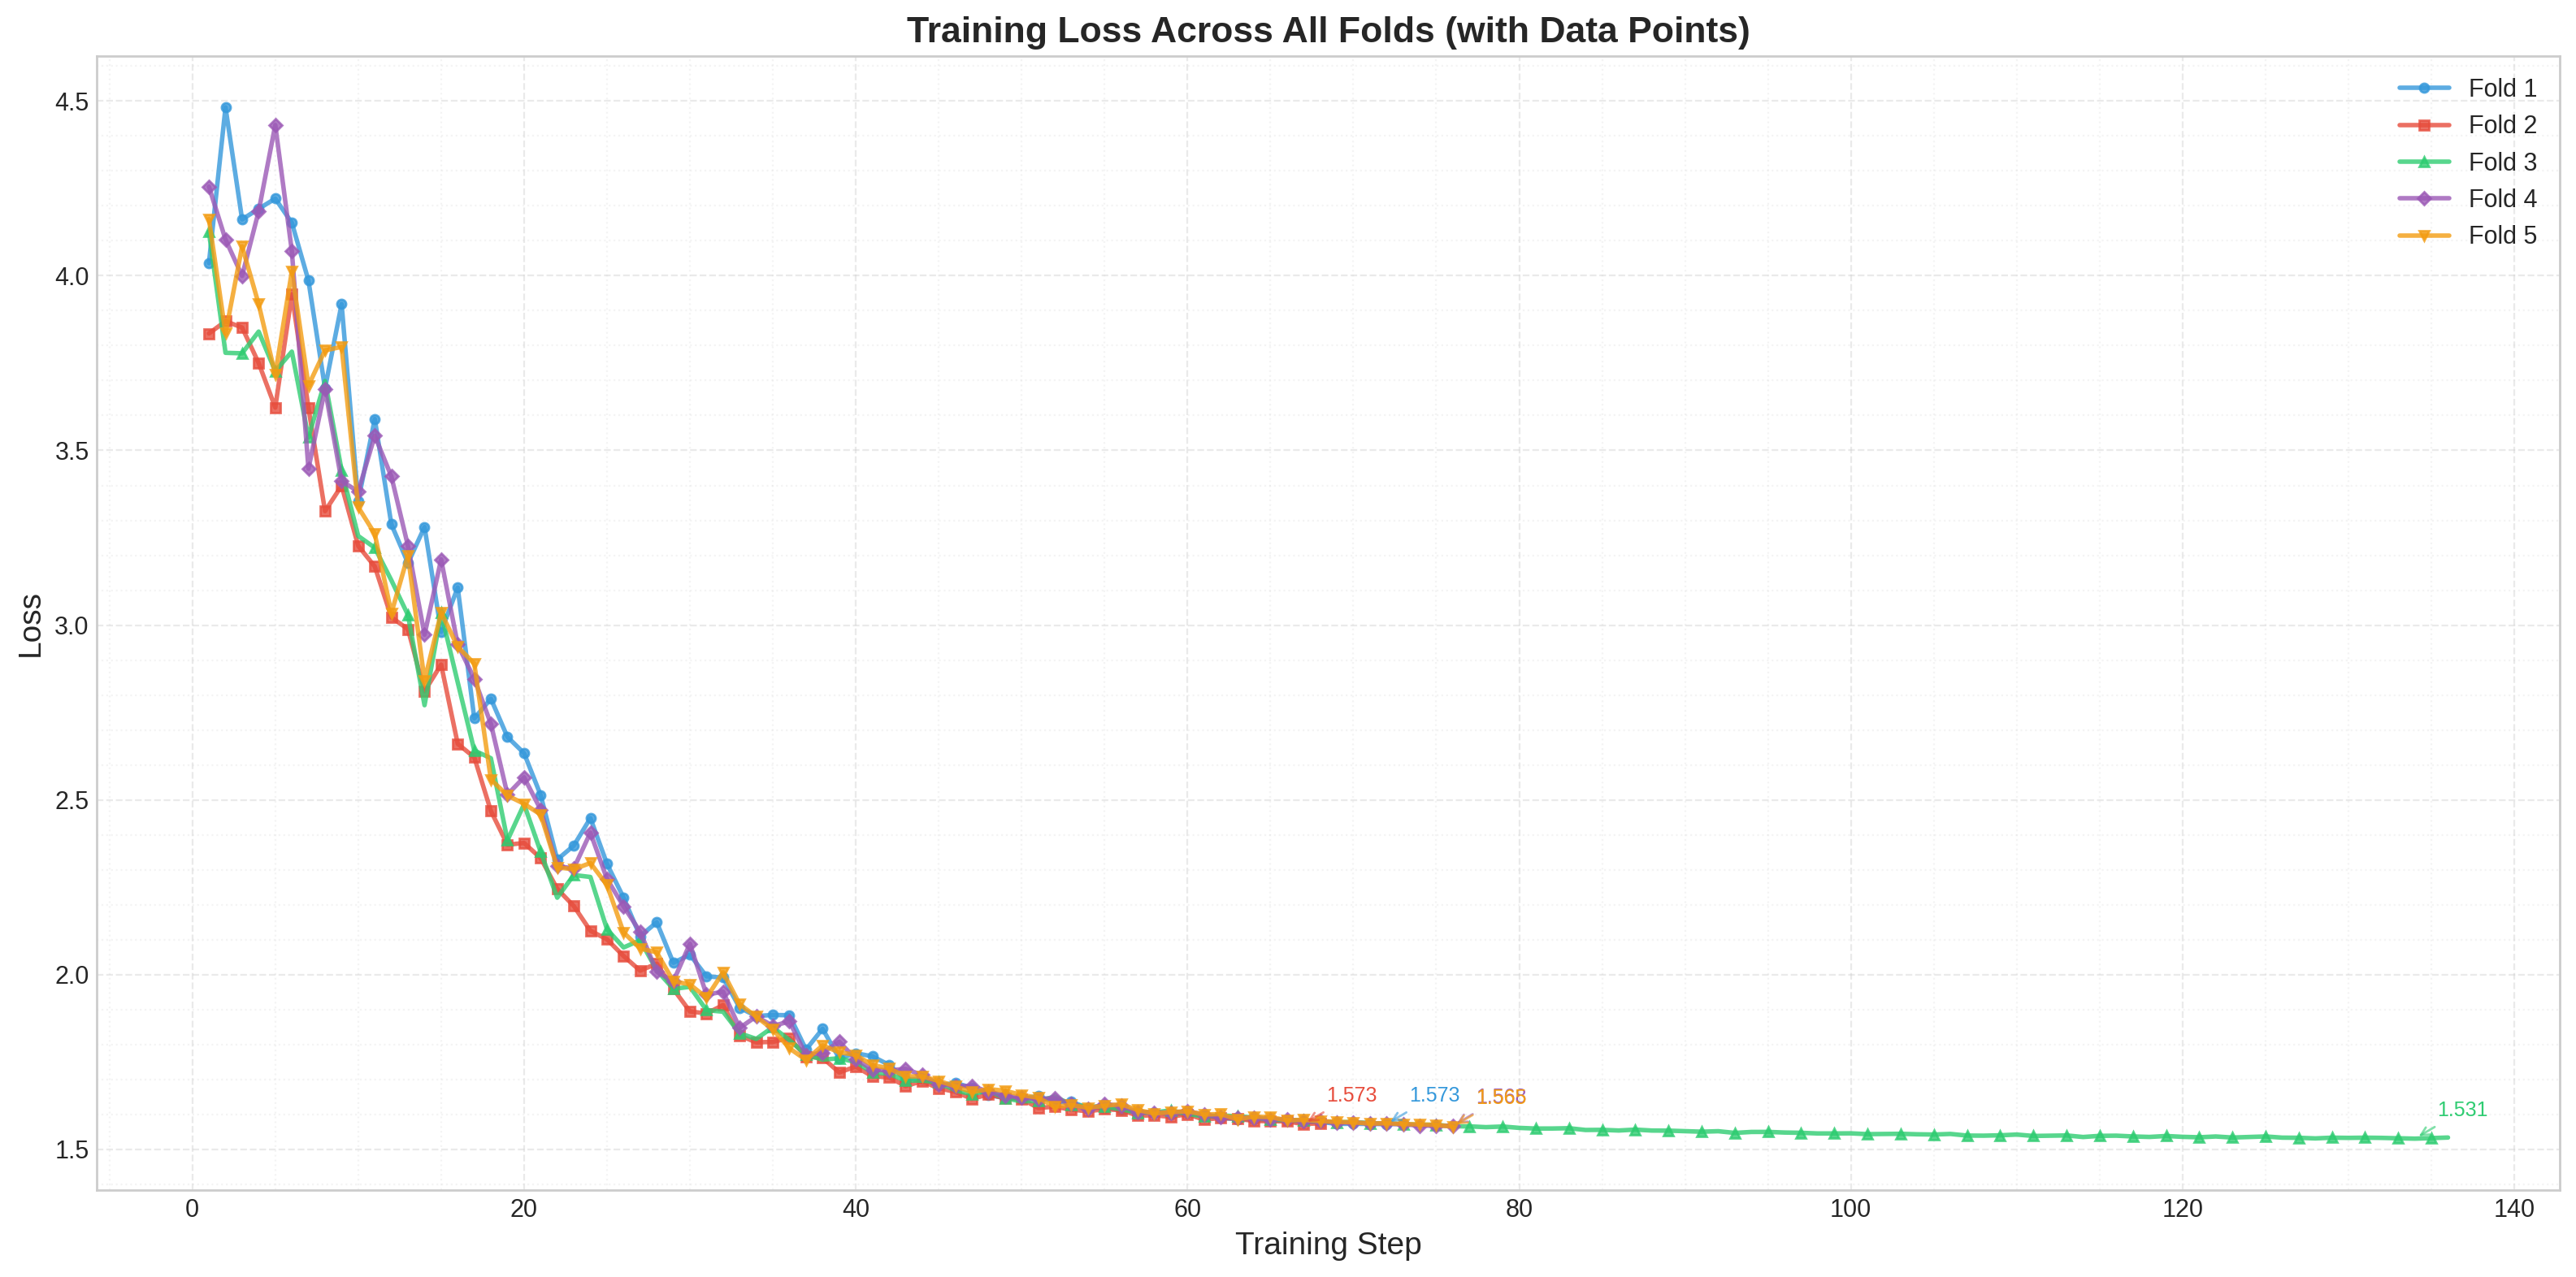
\includegraphics[width=0.8\textwidth]{code/lora/outputs/metrics/lora_20260212_063207/visualizations/training_loss_detailed.png}
\caption{Kurva Training Loss --- Strategi LoRA}
\label{fig:lora_training_loss}
\end{figure}

Tabel~\ref{tab:lora_training_summary} merangkum statistik training LoRA:

\begin{table}[H]
\centering
\caption{Ringkasan Training LoRA per Fold}
\label{tab:lora_training_summary}
\begin{tabular}{|c|c|c|c|c|}
\hline
\textbf{Fold} & \textbf{Steps} & \textbf{Initial Loss} & \textbf{Final Loss} & \textbf{Epoch} \\
\hline
0 & 72 & 4,036 & 1,573 & 18 \\
\hline
1 & 68 & 3,835 & 1,575 & 17 \\
\hline
2 & 136 & 4,126 & 1,534 & 34 \\
\hline
3 & 76 & 4,255 & 1,568 & 19 \\
\hline
4 & 76 & 4,162 & 1,565 & 19 \\
\hline
\hline
\textbf{Mean} & \textbf{85,6} & \textbf{4,083} & \textbf{1,563} & \textbf{21,4} \\
\hline
\end{tabular}
\end{table}

Pola konvergensi LoRA menunjukkan karakteristik yang berbeda dari \textit{Freeze Encoder}:

\begin{itemize}
    \item \textbf{Initial Loss yang Konsisten}: LoRA memulai dengan loss rata-rata 4,08 (rentang 3,84--4,26), mirip dengan \textit{Freeze Encoder} yang juga menggunakan \textit{label smoothing} (4,00--4,20). Kesamaan \textit{initial loss} ini diharapkan karena kedua strategi menggunakan \textit{label smoothing factor} yang sama (0,1) yang mendominasi nilai loss awal.
    
    \item \textbf{Final Loss Konvergen}: Loss akhir LoRA ($\sim$1,56) konvergen ke nilai yang serupa dengan \textit{Freeze Encoder} ($\sim$1,70), keduanya di sekitar batas minimum teoritis yang ditentukan oleh \textit{label smoothing}. Loss LoRA sedikit lebih rendah karena jumlah parameter trainable yang lebih kecil (1,47\% vs 50\%) memberikan regularisasi implisit tambahan \cite{szegedy2016rethinking}.
    
    \item \textbf{Konvergensi Cepat dengan \textit{Early Stopping}}: Rata-rata hanya memerlukan 85,6 \textit{steps} (21,4 epoch), jauh lebih sedikit dibanding \textit{Freeze Encoder} (111,2 \textit{steps}, 27,8 epoch). Namun \textit{Fold}~2 memerlukan 136 \textit{steps} (34 epoch), hampir dua kali lipat rata-rata \textit{fold} lainnya, menunjukkan bahwa fold ini memiliki distribusi data yang memerlukan waktu adaptasi lebih lama---dan justru menghasilkan performa terbaik.
    
    \item \textbf{Efisiensi Parameter}: Meskipun hanya melatih 1,47\% parameter (vs 50\%), LoRA mencapai WER rata-rata yang lebih baik (17,87\% vs 20,34\%). Hal ini menunjukkan bahwa \textit{low-rank adaptation} mampu mengekstraksi kapasitas pembelajaran yang cukup dari modifikasi parameter yang sangat terbatas.
\end{itemize}

\subsection{Metrik Evaluasi LoRA}

Gambar~\ref{fig:lora_eval_metrics} menunjukkan perkembangan WER dan CER selama evaluasi.

\begin{figure}[H]
\centering
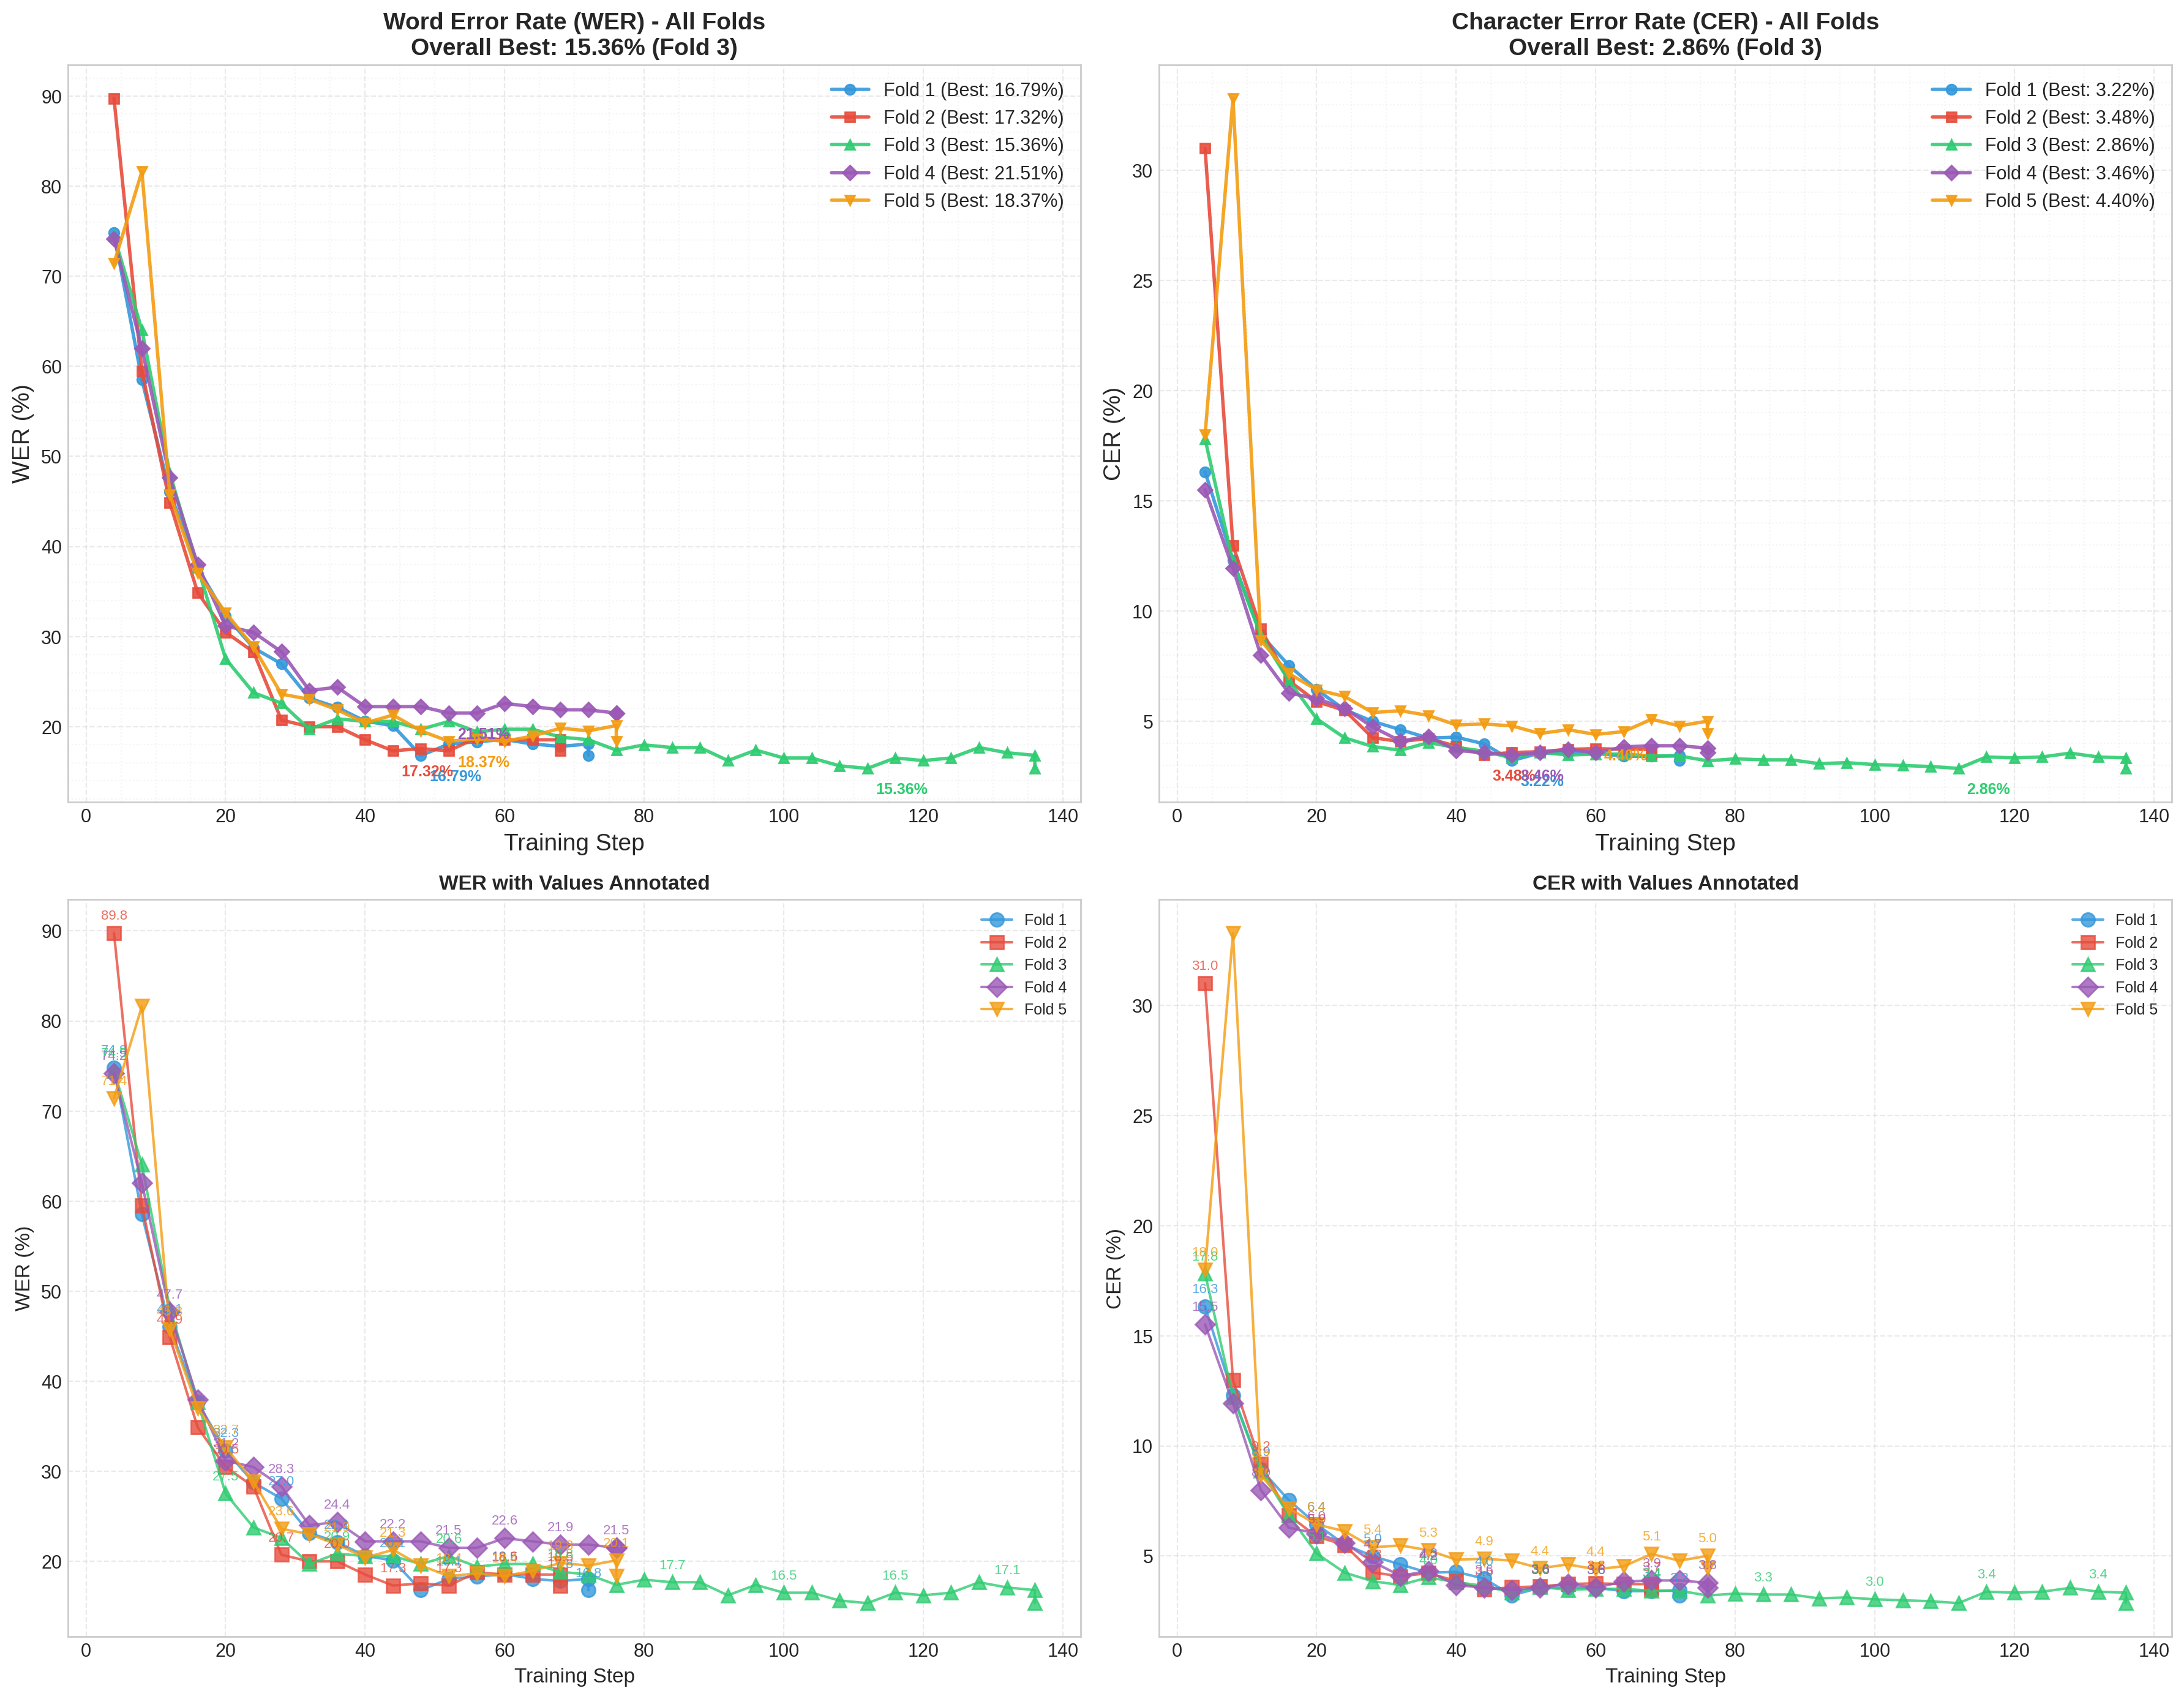
\includegraphics[width=0.9\textwidth]{code/lora/outputs/metrics/lora_20260212_063207/visualizations/evaluation_metrics_detailed.png}
\caption{Perkembangan WER dan CER --- Strategi LoRA}
\label{fig:lora_eval_metrics}
\end{figure}

Semua \textit{fold} menunjukkan penurunan WER dari rentang tinggi pada evaluasi awal menjadi 15--22\% pada evaluasi akhir. \textit{Fold}~2 yang memerlukan \textit{steps} terbanyak (136) menunjukkan kurva konvergensi yang lebih gradual, sementara \textit{fold} lainnya (68--76 \textit{steps}) konvergen lebih cepat. Konvergensi metrik evaluasi menunjukkan stabilitas yang baik tanpa fluktuasi berlebihan, konsisten dengan efek regularisasi dari \textit{label smoothing} dan jumlah parameter trainable yang sangat terbatas.

\subsection{Prediksi Model LoRA}

Tabel~\ref{tab:lora_predictions_fold2} menampilkan contoh prediksi pada \textit{Fold}~2 (fold terbaik WER, 15,36\%):

\begin{table}[H]
\centering
\caption{Contoh Prediksi LoRA pada Fold 2 (Fold Terbaik WER)}
\label{tab:lora_predictions_fold2}
\resizebox{\textwidth}{!}{%
\begin{tabular}{|p{0.42\textwidth}|p{0.42\textwidth}|c|c|}
\hline
\textbf{Referensi} & \textbf{Prediksi Model} & \textbf{WER} & \textbf{CER} \\
\hline
dalam deklarasi sadunia hak hak asasi manusia & 
dalam deklarasi sadunia hak hak asasi manusia & 
\textbf{0,0\%} & \textbf{0,0\%} \\
\hline
untuak mamajukan panghormatan taradok hak hak asasi manusia dan kamardekaan nan mandasar & 
untuak mamajukan panghormatan taradok hak hak asasi manusia dan kamardekaan nan mandasar & 
\textbf{0,0\%} & \textbf{0,0\%} \\
\hline
punyo hak mandapek linduangan masyarakat jo negara & 
punyo hak mandapek linduangan masyarakat jo negara & 
\textbf{0,0\%} & \textbf{0,0\%} \\
\hline
hak ko indak balaku untuak dakwaan kajahatan non politik & 
hak ko indak balaku untuak daquan kajahatan non politik & 
11,1\% & 5,4\% \\
\hline
\end{tabular}%
}
\end{table}

Sebagai perbandingan, Tabel~\ref{tab:lora_predictions_fold3} menampilkan contoh prediksi dari \textit{Fold}~3 (fold terburuk WER, 21,51\%):

\begin{table}[H]
\centering
\caption{Contoh Prediksi LoRA pada Fold 3 (Fold Terburuk WER)}
\label{tab:lora_predictions_fold3}
\resizebox{\textwidth}{!}{%
\begin{tabular}{|p{0.42\textwidth}|p{0.42\textwidth}|c|c|}
\hline
\textbf{Referensi} & \textbf{Prediksi Model} & \textbf{WER} & \textbf{CER} \\
\hline
hak hak ko adolah milik awak & 
hak hak ko adolah milik awak & 
\textbf{0,0\%} & \textbf{0,0\%} \\
\hline
hak hak asasi manusia paralu dijamin malalui tartib hukum & 
hak hak asasi manusia paralu dijamin malalui tartib hukum & 
\textbf{0,0\%} & \textbf{0,0\%} \\
\hline
kalompok atau sasaurang & 
kalompok atau saso urang & 
66,7\% & 8,7\% \\
\hline
baitu pulo kahormatan jo namo baiaknyo & 
baitu pulo kah rumah tan jo nan mo baiknyo & 
100,0\% & 18,4\% \\
\hline
\end{tabular}%
}
\end{table}

Pola kesalahan LoRA menunjukkan karakteristik yang khas:

\begin{enumerate}
    \item \textbf{Prediksi Sempurna}: Pada \textit{Fold}~2, 9 dari 31 sampel (29\%) diprediksi sempurna, sementara pada \textit{Fold}~3 hanya 5 dari 31 (16\%). Kalimat pendek cenderung diprediksi dengan benar.
    
    \item \textbf{Segmentasi Kata}: Kesalahan ``dakwaan'' $\rightarrow$ ``daquan'' dan ``sasaurang'' $\rightarrow$ ``saso urang'' menunjukkan tantangan dalam mengenali batas kata dan \textit{compound word} dalam bahasa Minangkabau. Kata ``sasaurang'' yang seharusnya satu kata dipecah menjadi dua kata oleh model.
    
    \item \textbf{Hallusinasi pada Kalimat Pendek}: Pada \textit{Fold}~3, prediksi ``kahormatan jo namo baiaknyo'' $\rightarrow$ ``kah rumah tan jo nan mo baiknyo'' (WER 100\%) menunjukkan \textit{hallucination} yang signifikan dimana model menghasilkan kata-kata yang secara fonetik mirip tetapi secara semantik berbeda. Ini merupakan tantangan khas pada dataset kecil.
    
    \item \textbf{CER Tetap Terkontrol}: Bahkan pada prediksi dengan WER tertinggi (100\%), CER tetap moderat (18,4\%), mengkonfirmasi bahwa kesalahan lebih bersifat \textit{word-level} daripada \textit{character-level}.
\end{enumerate}

%% ====================================================================
%% SECTION: PERBANDINGAN STRATEGI
%% ====================================================================
\section{Perbandingan Strategi Fine-Tuning} \label{IV.Perbandingan}

\subsection{Ringkasan Seluruh Percobaan}

Tabel~\ref{tab:all_runs_summary} menyajikan ringkasan hasil dari seluruh sepuluh percobaan (lima \textit{Freeze Encoder} dan lima LoRA) yang dilakukan selama penelitian.

\begin{table}[H]
\centering
\caption{Ringkasan Seluruh Percobaan Training}
\label{tab:all_runs_summary}
\resizebox{\textwidth}{!}{%
\begin{tabular}{|c|l|c|c|c|c|c|c|}
\hline
\textbf{No.} & \textbf{Strategi} & \textbf{LR} & \textbf{Batch} & \textbf{W. Decay} & \textbf{Beam} & \textbf{Mean WER (\%)} & \textbf{Mean CER (\%)} \\
\hline
\hline
\multicolumn{8}{|c|}{\textbf{Freeze Encoder}} \\
\hline
FE-1 & Freeze Encoder & 5$\times$10\textsuperscript{-6} & 16$\times$2 & 0,2 & 1 & 25,07 $\pm$ 2,86 & 5,60 $\pm$ 0,59 \\
\hline
FE-2 & Freeze Encoder & 1$\times$10\textsuperscript{-5} & 16$\times$2 & 0,2 & 1 & 22,34 $\pm$ 1,89 & 4,93 $\pm$ 0,55 \\
\hline
FE-3 & Freeze Encoder & 1$\times$10\textsuperscript{-5} & 16$\times$2 & 0,2 & 1 & 22,95 $\pm$ 2,70 & 5,52 $\pm$ 0,77 \\
\hline
FE-4 & Freeze Encoder & 1$\times$10\textsuperscript{-5} & 32$\times$1 & 0,1 & 5 & 19,92 $\pm$ 2,42 & 4,53 $\pm$ 0,65 \\
\hline
\textbf{FE-5} & \textbf{Freeze Encoder} & \textbf{1$\times$10\textsuperscript{-5}} & \textbf{32$\times$1} & \textbf{0,1} & \textbf{5} & \textbf{20,34 $\pm$ 2,41} & \textbf{4,46 $\pm$ 0,50} \\
\hline
\hline
\multicolumn{8}{|c|}{\textbf{LoRA}} \\
\hline
L-1 & LoRA ($r$=8) & 5$\times$10\textsuperscript{-4} & 32 & 0,01 & 5 & 17,32 $\pm$ 0,83 & 3,49 $\pm$ 0,43 \\
\hline
L-2 & LoRA ($r$=8) & 5$\times$10\textsuperscript{-4} & 32 & 0,01 & 5 & 17,73 $\pm$ 1,91 & 3,57 $\pm$ 0,33 \\
\hline
L-3 & LoRA ($r$=16) & 3$\times$10\textsuperscript{-4} & 32 & 0,03 & 5 & 18,03 $\pm$ 1,01 & 3,80 $\pm$ 0,39 \\
\hline
L-4 & LoRA ($r$=8) & 7$\times$10\textsuperscript{-4} & 32 & 0,05 & 5 & 17,43 $\pm$ 1,74 & 3,78 $\pm$ 0,53 \\
\hline
\textbf{L-5} & \textbf{LoRA ($r$=8)} & \textbf{7$\times$10\textsuperscript{-4}} & \textbf{32} & \textbf{0,05} & \textbf{5} & \textbf{17,87 $\pm$ 2,06} & \textbf{3,51 $\pm$ 0,53} \\
\hline
\end{tabular}%
}
\end{table}

Dari Tabel~\ref{tab:all_runs_summary}, terlihat jelas bahwa \textbf{seluruh percobaan LoRA} (WER 17,32\%--18,03\%) mengungguli \textbf{seluruh percobaan Freeze Encoder} (WER 19,92\%--25,07\%) dalam hal rata-rata WER. Bahkan percobaan LoRA terburuk (L-3, WER 18,03\%) masih lebih baik 1,89 poin persentase dari percobaan \textit{Freeze Encoder} terbaik (FE-4, WER 19,92\%). Hal ini menunjukkan keunggulan yang konsisten dan \textit{robust} dari strategi LoRA pada skenario \textit{low-resource} ini. Run terakhir pada masing-masing strategi (FE-5 dan L-5) dipilih sebagai konfigurasi final karena menggunakan \textit{label smoothing} dan konfigurasi regularisasi yang telah dioptimasi berdasarkan temuan Run 1--4.

\subsection{Perbandingan Metrik Utama}

Tabel~\ref{tab:strategy_comparison} menyajikan perbandingan komprehensif antara kedua strategi \textit{fine-tuning}.

\begin{table}[H]
\centering
\caption{Perbandingan Strategi Freeze Encoder vs LoRA}
\label{tab:strategy_comparison}
\resizebox{\textwidth}{!}{%
\begin{tabular}{|l|c|c|c|}
\hline
\textbf{Metrik} & \textbf{Freeze Encoder} & \textbf{LoRA} & \textbf{Selisih} \\
\hline
\hline
\multicolumn{4}{|c|}{\textbf{Performa}} \\
\hline
Mean WER (\%) & 20,34 $\pm$ 2,41 & \textbf{17,87 $\pm$ 2,06} & $\downarrow$ 2,47 pp \\
\hline
Mean CER (\%) & 4,46 $\pm$ 0,50 & \textbf{3,51 $\pm$ 0,53} & $\downarrow$ 0,95 pp \\
\hline
Best Fold WER (\%) & 16,81 & \textbf{15,36} & $\downarrow$ 1,45 pp \\
\hline
Worst Fold WER (\%) & 24,37 & \textbf{21,51} & $\downarrow$ 2,86 pp \\
\hline
Rentang WER (\%) & 7,56 & \textbf{6,15} & $\downarrow$ 1,41 pp \\
\hline
Std WER (\%) & 2,41 & \textbf{2,06} & $\downarrow$ 0,35 pp \\
\hline
\hline
\multicolumn{4}{|c|}{\textbf{Efisiensi}} \\
\hline
Parameter Trainable & $\sim$37M (50,0\%) & \textbf{$\sim$1,1M (1,47\%)} & 34$\times$ lebih efisien \\
\hline
Rata-rata Steps & 111,2 & \textbf{85,6} & $\downarrow$ 25,6 \\
\hline
Rata-rata Epoch & 27,8 & \textbf{21,4} & $\downarrow$ 6,4 \\
\hline
Learning Rate & 1$\times$10\textsuperscript{-5} & 7$\times$10\textsuperscript{-4} & 70$\times$ lebih tinggi \\
\hline
Weight Decay & 0,1 & 0,05 & 2$\times$ lebih ringan \\
\hline
Label Smoothing & 0,1 & 0,1 & Sama \\
\hline
Dropout (dec/attn/act) & 0,2 / 0,15 / 0,15 & 0,1 / 0,05 / 0,05 & Lebih ringan \\
\hline
\end{tabular}%
}
\end{table}

\subsection{Analisis Perbandingan}

Dari Tabel~\ref{tab:strategy_comparison}, dapat diidentifikasi beberapa temuan kunci:

\begin{enumerate}
    \item \textbf{LoRA Mengungguli Freeze Encoder pada Metrik Rata-Rata}: LoRA mencapai WER \cite{morris2004wer} 17,87\% dibandingkan 20,34\% pada \textit{Freeze Encoder} (penurunan relatif 12,1\%). Penurunan CER juga signifikan: 3,51\% vs 4,46\% (penurunan relatif 21,3\%). Keunggulan ini dicapai dengan hanya melatih 1,47\% parameter---34 kali lebih sedikit dari \textit{Freeze Encoder}.
    
    \item \textbf{LoRA Lebih Konsisten}: Standar deviasi WER LoRA (2,06\%) lebih rendah dibandingkan \textit{Freeze Encoder} (2,41\%), dan rentang WER antar-\textit{fold} LoRA (6,15 pp) juga lebih sempit dibanding \textit{Freeze Encoder} (7,56 pp). Meskipun perbedaan konsistensi tidak sedramatis pada konfigurasi sebelumnya, LoRA tetap menunjukkan stabilitas yang lebih baik.
    
    \item \textbf{LoRA Unggul pada Semua Fold}: Berbeda dengan perbandingan sebelumnya, LoRA kini juga mencapai \textit{best-case fold} yang lebih baik (15,36\% vs 16,81\%). Baik \textit{best-case} maupun \textit{worst-case} LoRA lebih baik dari \textit{Freeze Encoder}, mengkonfirmasi keunggulan yang konsisten di seluruh pembagian data.
    
    \item \textbf{Konvergensi Lebih Cepat}: LoRA rata-rata memerlukan 85,6 \textit{steps} (21,4 epoch) dibandingkan \textit{Freeze Encoder} yang memerlukan 111,2 \textit{steps} (27,8 epoch). Konvergensi yang lebih cepat ini konsisten dengan \textit{learning rate} yang lebih tinggi (70$\times$) dan jumlah parameter trainable yang lebih kecil.
    
    \item \textbf{Strategi Regularisasi Berbeda}: Kedua strategi kini menggunakan \textit{label smoothing} yang sama (0,1), namun \textit{Freeze Encoder} masih memerlukan \textit{dropout} dan \textit{weight decay} yang lebih tinggi karena 50\% parameter yang dilatih berisiko \textit{overfitting} pada dataset kecil. LoRA menggunakan regularisasi yang lebih ringan karena \textit{low-rank constraint} ($r$=8) sendiri sudah berfungsi sebagai regularisasi struktural yang membatasi kapasitas model secara inheren \cite{hu2022lora}.
\end{enumerate}

Gambar~\ref{fig:comparison_cv} mengilustrasikan perbandingan visual performa kedua strategi.

\begin{figure}[H]
\centering
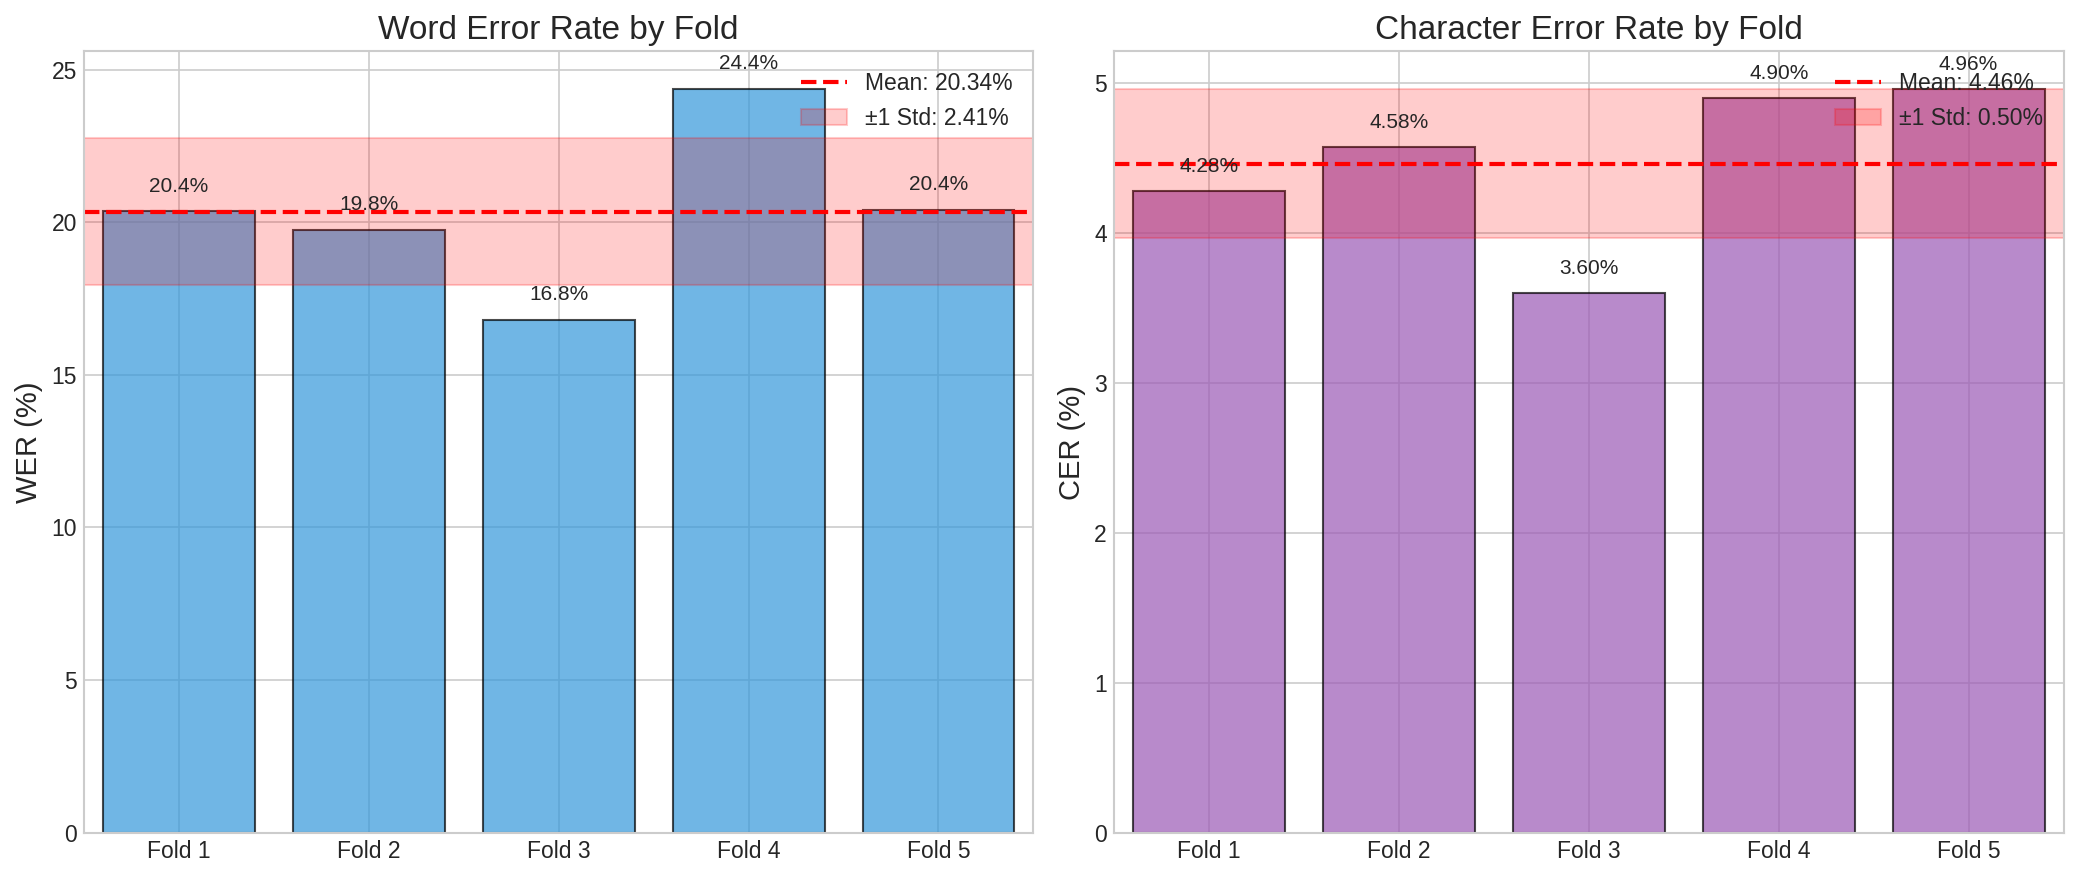
\includegraphics[width=0.9\textwidth]{code/freeze_encoder/outputs/metrics/run_20260212_060037/visualizations/cross_validation_summary.png}
\caption{Cross-Validation Summary --- Freeze Encoder}
\label{fig:comparison_cv}
\end{figure}

\begin{figure}[H]
\centering
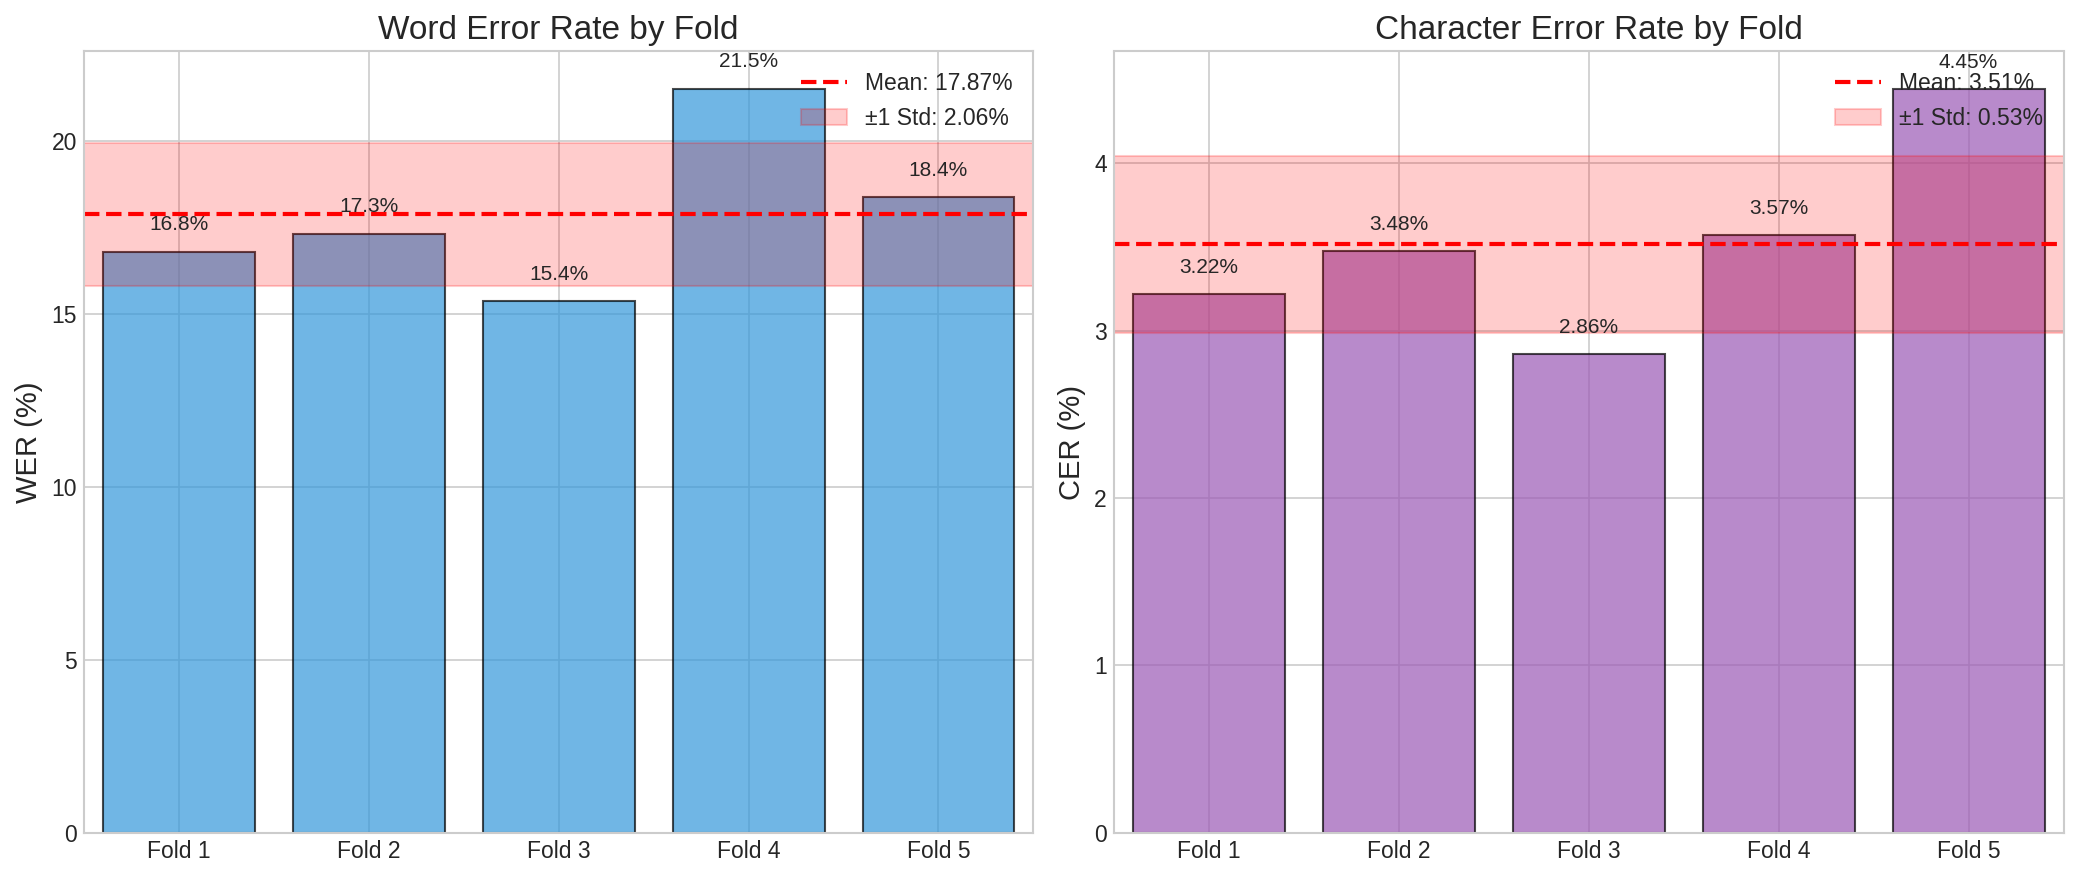
\includegraphics[width=0.9\textwidth]{code/lora/outputs/metrics/lora_20260212_063207/visualizations/cross_validation_summary.png}
\caption{Cross-Validation Summary --- LoRA}
\label{fig:lora_cv_summary}
\end{figure}

%% ====================================================================
%% SECTION: PEMBAHASAN
%% ====================================================================
\section{Pembahasan} \label{IV.Analisis}

\subsection{Efektivitas LoRA pada Skenario Low-Resource}

Keunggulan LoRA atas \textit{Freeze Encoder} pada skenario \textit{extremely low-resource} (1,3 jam) merupakan temuan yang signifikan dan sedikit bertentangan dengan intuisi awal. Secara konvensional, lebih banyak parameter trainable (50\% pada \textit{Freeze Encoder}) seharusnya memberikan kapasitas belajar yang lebih besar. Namun, hasil dari seluruh sepuluh percobaan (lima \textit{Freeze Encoder} dan lima LoRA, lihat Tabel~\ref{tab:all_runs_summary}) secara konsisten menunjukkan sebaliknya---LoRA dengan hanya 1,47\% parameter trainable justru lebih baik pada setiap konfigurasi yang diuji. Beberapa penjelasan untuk fenomena ini:

\begin{itemize}
    \item \textbf{Regularisasi Struktural}: \textit{Low-rank constraint} ($r$=8) membatasi perubahan representasi internal ke subspace berdimensi rendah, secara efektif mencegah \textit{overfitting} tanpa memerlukan regularisasi eksplisit yang agresif. Hal ini krusial pada dataset kecil di mana \textit{overfitting} merupakan risiko utama \cite{hu2022lora}.
    
    \item \textbf{Adaptasi di Seluruh Layer}: LoRA memodifikasi semua 6 \textit{linear layer} di setiap blok transformer (encoder dan decoder), memberikan adaptasi yang terdistribusi merata. Sebaliknya, \textit{Freeze Encoder} hanya memodifikasi decoder, sehingga representasi encoder tetap statis. Meskipun encoder Whisper sudah baik untuk audio umum, adaptasi ringan melalui LoRA pada encoder dapat meningkatkan representasi fitur spesifik untuk karakteristik akustik bahasa Minangkabau.
    
    \item \textbf{Learning Rate Optimal}: LoRA menggunakan learning rate 70$\times$ lebih tinggi (7$\times$10\textsuperscript{-4} vs 1$\times$10\textsuperscript{-5}), yang dimungkinkan oleh jumlah parameter trainable yang sangat kecil. Learning rate yang lebih tinggi memungkinkan adaptasi yang lebih cepat dan eksplorasi ruang parameter yang lebih efektif.
    
    \item \textbf{Label Smoothing}: Penggunaan \textit{label smoothing} (0,1) pada kedua strategi mendistribusikan probabilitas ke seluruh \textit{vocabulary}, mencegah model menjadi terlalu percaya diri dan meningkatkan kalibrasi probabilistik \cite{szegedy2016rethinking}. Teknik ini berkontribusi pada stabilitas performa antar-\textit{fold} pada kedua metode.
\end{itemize}

\subsection{Konsistensi sebagai Indikator Generalisasi}

Konsistensi LoRA (std WER 2,06\% vs 2,41\%) merupakan keunggulan yang relevan untuk sistem ASR \textit{low-resource}:

\begin{itemize}
    \item Pada skenario \textit{deployment}, variasi performa yang tinggi berarti pengguna mungkin mendapatkan pengalaman yang sangat berbeda tergantung pada konten audio. Model dengan konsistensi tinggi memberikan pengalaman pengguna yang lebih dapat diprediksi.
    
    \item Rentang WER LoRA (15,36\%--21,51\%) lebih sempit dibandingkan \textit{Freeze Encoder} (16,81\%--24,37\%), menunjukkan bahwa model LoRA generalize dengan lebih baik terhadap berbagai pembagian data.
    
    \item Keunggulan LoRA pada \textit{best-case fold} (15,36\% vs 16,81\%) maupun \textit{worst-case fold} (21,51\% vs 24,37\%) mengkonfirmasi bahwa performa yang baik bukan hasil dari pembagian data yang ``beruntung'', melainkan superioritas metode yang konsisten.
\end{itemize}

\subsection{Efisiensi Komputasi}

Kedua strategi menunjukkan efisiensi komputasi yang baik pada GPU RTX 5060 Ti 16GB:

\begin{itemize}
    \item \textbf{Freeze Encoder}: Rata-rata 111,2 \textit{steps} (27,8 epoch) per \textit{fold}. Melatih $\sim$37M parameter dengan BF16 \textit{mixed precision} \cite{micikevicius2018mixed}.
    
    \item \textbf{LoRA}: Rata-rata 85,6 \textit{steps} (21,4 epoch) per \textit{fold}. Melatih hanya $\sim$1,1M parameter namun dengan \textit{overhead adapter} \cite{manmatha2017peft} pada 6 layer per blok.
    
    \item \textbf{Efisiensi Parameter}: LoRA mencapai WER 12\% lebih baik dengan parameter 34$\times$ lebih sedikit dan \textit{steps} rata-rata yang lebih rendah. Dalam konteks \textit{low-resource language} di mana data sangat mahal untuk dikumpulkan, efisiensi parameter LoRA sangat berharga karena memungkinkan adaptasi cepat ke bahasa baru tanpa risiko \textit{overfitting} yang signifikan.
\end{itemize}

\subsection{Transfer Learning dan Kedekatan Tipologis}

Keberhasilan kedua strategi---terutama LoRA yang hanya memodifikasi 1,47\% parameter---mengkonfirmasi efektivitas \textit{transfer learning} \cite{pan2010transfer} dari Whisper yang dilatih pada 680.000 jam audio multibahasa. Penggunaan bahasa Indonesia (\texttt{id}) sebagai \textit{proxy language token} untuk bahasa Minangkabau terbukti efektif berkat kedekatan tipologis antara kedua bahasa rumpun Austronesia \cite{koto2020minangkabau,liang2025fieldmatters}.

Hasil ini konsisten dengan temuan penelitian terdahulu: Pillai dkk. \cite{pillai2024multistage} mencapai WER $\sim$25\% pada bahasa Malaysia dengan \textit{multi-stage fine-tuning}; Gete dkk. \cite{gete2025whispering} melaporkan WER kompetitif pada bahasa Basque dengan pendekatan serupa; dan Li dkk. \cite{li2024improving} menunjukkan efektivitas LoRA pada bahasa Tionghoa \textit{low-resource}. Performa LoRA pada penelitian ini (WER 17,87\%) tergolong sangat baik mengingat keterbatasan data ($\sim$1,3 jam) yang jauh lebih kecil dari dataset pada penelitian-penelitian tersebut.

\subsection{Limitasi dan Tantangan}

Beberapa limitasi yang berlaku untuk kedua strategi:

\begin{itemize}
    \item \textbf{Ukuran Dataset}: Dataset 1,3 jam sangat terbatas untuk bahasa dengan variasi dialek luas seperti Minangkabau \cite{liang2025fieldmatters,pratap2020mls}. Peningkatan signifikan diharapkan ketika data bertambah menjadi 5--10 jam.
    
    \item \textbf{Standarisasi Ortografi}: Ketiadaan standar ejaan resmi untuk bahasa Minangkabau menyebabkan inkonsistensi transkripsi yang secara artifisial meningkatkan WER \cite{koto2020minangkabau,sovia2022minangkabau}. Variasi seperti ``di antaro'' vs ``diantaro'' dihitung sebagai kesalahan meskipun secara semantik benar.
    
    \item \textbf{Potensi Estimasi Optimistis}: Penggunaan \textit{evaluation set} yang sama untuk \textit{early stopping} dan pelaporan metrik berpotensi menghasilkan estimasi performa yang sedikit optimistis pada kedua strategi. Namun, penggunaan 5-\textit{fold cross-validation} memitigasi risiko ini dibandingkan evaluasi \textit{single split}.
    
    \item \textbf{Domain Spesifik}: Data dari LibriVox (pembacaan teks) mungkin tidak merepresentasikan percakapan spontan, membatasi generalisasi domain.
    
    \item \textbf{Ruang Hyperparameter}: Meskipun lima percobaan dilakukan pada masing-masing strategi, eksplorasi \textit{hyperparameter} yang lebih luas (misalnya variasi \textit{rank} LoRA yang lebih ekstrem, \textit{learning rate scheduling} alternatif, atau \textit{data augmentation} yang berbeda) berpotensi menghasilkan performa yang lebih baik lagi.
\end{itemize}

    \newpage
\chapter{KESIMPULAN DAN SARAN} \label{Bab V}

\section{Kesimpulan} \label{V.Kesimpulan}

Penelitian ini telah berhasil mengadaptasi model \textit{Automatic Speech Recognition} (ASR) OpenAI Whisper Base untuk bahasa Minangkabau melalui \textit{fine-tuning} dengan dua strategi yang berbeda. Berdasarkan serangkaian 18 percobaan eksperimen dan analisis menyeluruh yang disajikan pada Bab~\ref{Bab IV}, kesimpulan penelitian ini disusun untuk menjawab kelima poin rumusan masalah secara berurutan.

\begin{enumerate}

    \item \textbf{Adaptasi Whisper Base untuk Bahasa Minangkabau (\textit{Low-Resource})}

    Model Whisper Base berhasil diadaptasi untuk mengenali ucapan bahasa Minangkabau melalui proses \textit{fine-tuning} pada dataset \textit{extremely low-resource} (156 file audio, $\sim$1,3 jam). Strategi adaptasi terbaik yang ditemukan merupakan kombinasi dari: (a) pemilihan \textit{hyperparameter} yang tepat melalui eksplorasi iteratif selama sembilan percobaan per strategi, (b) augmentasi data yang terkalibrasi (\textit{speed perturbation} 0,85--1,15, \textit{SpecAugment} minimal, \textit{pitch shifting}), (c) regularisasi berlapis (\textit{label smoothing} 0,1, \textit{weight decay} minimal, \textit{dropout} adaptif), dan (d) penerapan \textit{Weighted Cross-Entropy} (WCE) yang dirancang berdasarkan analisis pola kesalahan historis untuk memperkuat sinyal gradien pada token-token yang sulit.

    Penggunaan \textit{language token} bahasa Indonesia (\texttt{id}) sebagai \textit{proxy} terbukti efektif memanfaatkan kedekatan tipologis antara bahasa Indonesia dan bahasa Minangkabau sebagai sesama anggota rumpun Austronesia \cite{koto2020minangkabau}. Pendekatan \textit{transfer learning} ini memungkinkan model memanfaatkan representasi fonotaktik dan leksikal yang sudah dipelajari tanpa perlu pelatihan dari nol, sehingga keterbatasan data (1,3 jam) dapat diatasi secara signifikan.

    \item \textbf{Implementasi Sistem ASR Berbasis Python, PyTorch, dan Hugging Face Transformers}

    Sistem ASR bahasa Minangkabau berhasil dirancang dan diimplementasikan menggunakan ekosistem \textit{open-source}: Python sebagai bahasa pemrograman utama, PyTorch sebagai \textit{framework} \textit{deep learning}, Hugging Face Transformers untuk manajemen model dan \textit{tokenizer}, serta PEFT (\textit{Parameter-Efficient Fine-Tuning}) library untuk implementasi LoRA. \textit{Pipeline} yang dibangun mencakup modul \textit{audio preprocessing} (konversi format, \textit{resampling} ke 16 kHz, validasi durasi), \textit{text preprocessing} (normalisasi teks Minangkabau), augmentasi data (\textit{SpecAugment}, \textit{speed perturbation}, \textit{noise injection}), dan infrastruktur \textit{training} dengan \textit{monitoring} real-time melalui \textit{Weights \& Biases}. Seluruh kode diimplementasikan dengan desain modular yang memungkinkan konfigurasi fleksibel dan reprodusibilitas eksperimen.

    \item \textbf{Perbandingan Strategi \textit{Freeze Encoder} vs LoRA}

    Perbandingan komprehensif antara dua strategi \textit{fine-tuning} menghasilkan temuan-temuan berikut:

    \begin{enumerate}

        \item \textbf{LoRA unggul secara konsisten}: Strategi LoRA (L-9) mencapai WER rata-rata \textbf{16,33\% $\pm$ 2,03\%} dan CER \textbf{3,37\% $\pm$ 0,35\%}, mengungguli strategi \textit{Freeze Encoder} terbaik (FE-9) yang mencapai WER \textbf{18,24\% $\pm$ 2,18\%} dan CER \textbf{3,87\% $\pm$ 0,61\%}. Keunggulan LoRA bersifat \textit{robust} dan sistematis: seluruh rentang WER percobaan LoRA (16,33\%--18,37\%) berada di bawah atau sebanding dengan percobaan \textit{Freeze Encoder} terbaik.

        \item \textbf{Efisiensi parameter LoRA sangat signifikan}: LoRA (L-9, \textit{rank} 16) hanya melatih $\sim$2,93\% parameter ($\sim$2,16 juta dari 74 juta total), 17 kali lebih efisien dari \textit{Freeze Encoder} yang melatih 50\% parameter ($\sim$37 juta). Meskipun demikian, LoRA menghasilkan WER rata-rata yang 1,91 poin persentase lebih rendah dan \textit{worst-case fold} yang 3,90 poin persentase lebih baik (18,32\% vs 22,22\%).

        \item \textbf{\textit{Best single-fold} dicapai oleh LoRA}: L-9 Fold~4 mencapai WER \textbf{12,83\%} dan L-9 Fold~2 mencapai CER \textbf{2,77\%}, merupakan nilai terbaik di antara seluruh 18 percobaan dan 90 evaluasi fold yang dilakukan.

        \item \textbf{WCE memberikan peningkatan bertahap}: Penerapan \textit{Weighted Cross-Entropy} pada fase akhir (Run 7--9) berkontribusi pada penurunan WER sebesar 1,68 poin persentase pada \textit{Freeze Encoder} (dari FE-4: 19,92\% ke FE-9: 18,24\%) dan 0,99 poin persentase pada LoRA (dari L-1: 17,32\% ke L-9: 16,33\%). WCE paling efektif ketika dikombinasikan dengan jumlah \textit{training steps} yang cukup ($\geq$400) dan konfigurasi \textit{hyperparameter} yang optimal \cite{pineiromartin2024weighted}.

        \item \textbf{Augmentasi perlu dikalibrasi hati-hati}: Augmentasi berlebihan (FE-5, WER 21,14\%; L-5, WER 18,37\%) secara konsisten menurunkan performa dibandingkan konfigurasi augmentasi standar, mengkonfirmasi bahwa pada dataset sangat terbatas, keseimbangan antara diversifikasi data dan preservasi informasi linguistik sangat kritis.

    \end{enumerate}

    \item \textbf{Evaluasi dan Analisis Kesalahan Model}

    Evaluasi menggunakan skema 5-\textit{fold cross-validation} menghasilkan estimasi performa yang andal dan tidak bias. Analisis kualitatif terhadap prediksi model mengidentifikasi tiga pola kesalahan dominan yang bersifat sistematis:

    \begin{enumerate}
        \item \textbf{Substitusi fonetik}: Penggantian konsonan dengan artikulasi serupa (contoh: \textit{paralu} $\rightarrow$ \textit{palu}, \textit{barontak} $\rightarrow$ \textit{barantak}, \textit{kazaliman} $\rightarrow$ \textit{kajaliman}, \textit{mandorong} $\rightarrow$ \textit{mandaurang}). Pola ini dominan pada strategi \textit{Freeze Encoder} dan mencerminkan keterbatasan representasi akustik dari encoder yang dibekukan dalam membedakan konsonan-konsonan yang memiliki kemiripan akustik tinggi dalam bahasa Minangkabau.

        \item \textbf{Segmentasi kata}: Kesalahan pada batas kata (\textit{kaadilan} $\rightarrow$ \textit{ka adilan}, \textit{mangukuahkan} $\rightarrow$ \textit{manguku hakkan}), mencerminkan tantangan intrinsik yang belum sepenuhnya terselesaikan oleh kedua strategi. Fenomena ini berkaitan dengan ketiadaan standar ortografi resmi bahasa Minangkabau.

        \item \textbf{Substitusi vokal}: Pengubahan bunyi vokal pada suku kata tertentu (contoh: \textit{elok} $\rightarrow$ \textit{elo}), bersifat ringan dengan kontribusi kecil pada CER.
    \end{enumerate}

    Dibandingkan dengan \textit{Freeze Encoder}, \textit{Fold}~4 dari LoRA L-9 berhasil memprediksi sempurna (WER 0\%, CER 0\%) sejumlah kalimat panjang yang kompleks, membuktikan efektivitas adaptasi LoRA di seluruh lapisan encoder dan decoder model.

    \item \textbf{Kontribusi terhadap Pelestarian Bahasa Daerah}

    Penelitian ini berhasil menghasilkan prototipe sistem ASR bahasa Minangkabau pertama berbasis Whisper dengan WER 16,33\% pada domain pembacaan formal. Kontribusi utama terhadap pelestarian bahasa daerah mencakup: (1) terbentuknya \textit{pipeline} teknis yang sepenuhnya terdokumentasi dan dapat direproduksi untuk adaptasi model ASR ke bahasa-bahasa daerah Indonesia lain yang juga \textit{low-resource}, (2) penyediaan \textit{baseline} performa kuantitatif (WER 16,33\%, CER 3,37\%) yang dapat dijadikan titik acuan bagi penelitian lanjutan, (3) demonstrasi bahwa dengan hanya $\sim$1,3 jam data audio, sistem ASR fungsional untuk bahasa daerah dapat dibangun menggunakan metode PEFT yang efisien secara komputasi \cite{hu2022lora, gupta2024parameter}, serta (4) dokumentasi pola kesalahan sistematis yang dapat memandu pengembangan dataset dan standarisasi ortografi bahasa Minangkabau di masa depan \cite{koto2020minangkabau, sovia2022minangkabau}.

\end{enumerate}

Secara keseluruhan, penelitian ini menunjukkan bahwa \textit{fine-tuning} Whisper Base dengan strategi LoRA merupakan pendekatan yang paling efektif dan efisien untuk skenario ASR bahasa \textit{low-resource} seperti bahasa Minangkabau. Keunggulan LoRA tidak hanya terletak pada efisiensi parameter, tetapi juga pada kemampuannya menghasilkan adaptasi yang lebih menyeluruh dengan risiko \textit{overfitting} yang lebih rendah melalui regularisasi struktural dari \textit{low-rank constraint} \cite{hu2022lora, song2024lorawhisper}.

%% ===================================================================

\section{Saran} \label{V.Saran}

Berdasarkan temuan dan limitasi yang diidentifikasi dalam penelitian ini, berikut adalah saran-saran untuk pengembangan lebih lanjut:

\begin{enumerate}

    \item \textbf{Perluasan dan Diversifikasi Dataset}

    Keterbatasan utama penelitian ini adalah ukuran dan domain dataset yang sangat spesifik (1,3 jam, pembacaan teks formal UDHR). Penelitian lanjutan sangat disarankan untuk: (a) mengumpulkan data percakapan spontan, podcast, siaran radio, dan konten \textit{informal} dalam bahasa Minangkabau guna meningkatkan generalisasi model; (b) merepresentasikan variasi dialek regional Minangkabau (mis. dialek Agam, Lima Puluh Kota, Pasaman) yang masing-masing memiliki karakteristik fonetik berbeda; serta (c) mengembangkan standar anotasi dan ortografi untuk transkripsi bahasa Minangkabau agar konsistensi data training dapat ditingkatkan dan nilai WER tidak lagi dipengaruhi oleh inkonsistensi ejaan.

    \item \textbf{Eksplorasi Varian Model yang Lebih Besar}

    Penelitian ini dibatasi pada Whisper Base (74M parameter) karena risiko \textit{overfitting} pada dataset 1,3 jam. Seiring bertambahnya ketersediaan data, varian Whisper Small (244M) atau Medium (769M) berpotensi menghasilkan WER yang lebih rendah karena kapasitas representasi yang lebih besar. Dengan strategi LoRA, biaya komputasi untuk melatih varian lebih besar tetap terjangkau karena hanya $<$3\% parameter yang dilatih, sehingga eksplorasi ini layak dilakukan bahkan dengan data tambahan yang relatif terbatas.

    \item \textbf{Penerapan \textit{Multi-Stage Fine-Tuning}}

    Strategi \textit{multi-stage fine-tuning} yang pertama kali melatih model pada bahasa Indonesia (yang lebih banyak datanya) sebelum melakukan adaptasi akhir ke bahasa Minangkabau berpotensi meningkatkan performa secara signifikan \cite{pillai2024multistage}. Kedekatan tipologis antara bahasa Indonesia dan Minangkabau menjadikan transfer bertahap ini lebih efektif dibandingkan adaptasi langsung dari model multibahasa ke bahasa Minangkabau. Pendekatan ini juga dapat dikombinasikan dengan \textit{data augmentation} yang lebih agresif pada tahap pelatihan bahasa Indonesia.

    \item \textbf{Integrasi \textit{Language Model} pada Tahap \textit{Decoding}}

    Penelitian ini hanya menggunakan \textit{beam search} standar pada tahap \textit{decoding} tanpa \textit{external language model}. Arisaputra dan Zahra \cite{arisaputra2022xlsr53} menunjukkan bahwa integrasi \textit{language model} berbasis KenLM 4-gram menurunkan WER bahasa Indonesia dari $\sim$20\% ke $\sim$12\%, mengindikasikan potensi perbaikan yang serupa untuk bahasa Minangkabau. Pembangunan \textit{language model} bahasa Minangkabau dari sumber teks yang tersedia (Wikipedia, teks sastra digital, majalah daerah) dapat menjadi langkah praktis yang berdampak besar tanpa memerlukan data audio tambahan.

    \item \textbf{Penerapan Teknik Regularisasi dan Optimisasi Lanjutan}

    Beberapa teknik yang belum dieksplor dalam penelitian ini dan berpotensi meningkatkan performa di antaranya: (a) \textit{monotonic alignment loss} \cite{zhuang2025monotonic} yang secara eksplisit mengoptimalkan keselarasan antara sekuens audio dan teks selama \textit{fine-tuning}; (b) \textit{Mixture of LoRA Experts} \cite{bagat2025mixture} untuk menangani variasi dialek dalam satu model secara adaptif; serta (c) \textit{curriculum learning} yang menyajikan sampel dari yang mudah ke sulit selama pelatihan, membantu model membangun representasi secara bertahap pada dataset yang sangat terbatas \cite{liang2025fieldmatters}.

    \item \textbf{Perbaikan Metodologi Evaluasi}

    Untuk menghilangkan potensi bias dari penggunaan \textit{evaluation set} yang sama untuk \textit{early stopping} dan pelaporan, penelitian lanjutan disarankan untuk menggunakan skema evaluasi yang lebih ketat: (a) memisahkan \textit{validation set} dari \textit{training set} dalam setiap \textit{fold} ketika ukuran dataset sudah cukup besar ($>$5 jam), atau (b) menggunakan \textit{held-out test set} yang sama sekali tidak disentuh selama proses \textit{training} untuk evaluasi akhir yang benar-benar independen.

    \item \textbf{Pengembangan ke Sistem \textit{End-to-End}}

    Prototipe yang dihasilkan dalam penelitian ini merupakan komponen model saja. Untuk menghasilkan dampak praktis yang lebih besar terhadap pelestarian dan pengembangan bahasa Minangkabau, penelitian lanjutan dapat mengintegrasikan model ini ke dalam sistem yang lebih lengkap, misalnya: (a) aplikasi transkripsi berbasis web atau \textit{mobile} yang memungkinkan masyarakat Minangkabau mengunggah rekaman audio dan mendapatkan transkripsi otomatis; (b) alat bantu pembuatan \textit{subtitle} untuk konten video berbahasa Minangkabau; atau (c) sistem digitalisasi arsip audio budaya (rekaman \textit{kaba}, cerita rakyat, lagu tradisional) yang dapat diakses dan ditelusuri secara digital.

\end{enumerate}
	%----------------------------------------------------------------%
    % Daftar Pustaka
    \newpage
    \phantomsection%
    \addcontentsline{toc}{chapter}{DAFTAR PUSTAKA}
    \printbibliography[title={Daftar Pustaka}]
	%----------------------------------------------------------------%
    % Lampiran
    %----------------------------------------------------------------%
    % TODO: Tabel Lampiran
    \newpage
    \appendix
    \addcontentsline{toc}{chapter}{LAMPIRAN}
    \chapter*{Lampiran}
    \renewcommand\thesection{\Alph{section}}
    \section{Dataset}
Dataset yang digunakan dalam penelitian ini adalah dataset publik LibriVox Indonesia versi 1.0 yang disediakan oleh \textit{Indonesian-nlp} melalui platform Hugging Face (\url{https://huggingface.co/datasets/indonesian-nlp/librivox-indonesia}).

Dataset ini terdiri dari audio berformat MP3 dan file teks transkrip terkait yang dihasilkan dari buku-buku audio domain publik LibriVox. Pengumpulan data dalam repositori tersebut difokuskan secara khusus pada bahasa-bahasa di Indonesia. Durasi asli buku audio LibriVox bervariasi dari beberapa menit hingga beberapa jam. Namun, pada dataset ini, setiap file audio telah disegmentasi sehingga memiliki durasi mulai dari beberapa detik hingga maksimal 20 detik.

Konversi buku audio tersebut menjadi dataset ucapan dilakukan menggunakan perangkat lunak penyelarasan paksa (\textit{forced alignment}) yang dikembangkan oleh pihak pengembang. Perangkat lunak ini dirancang untuk mendukung multibahasa, termasuk bahasa-bahasa dengan sumber daya terbatas (\textit{low-resource}), seperti Aceh, Bali, maupun Minangkabau, tanpa memerlukan pekerjaan tambahan untuk melatih model penjajaran. Secara keseluruhan, dataset dari repositori utama saat ini terdiri dari total 8 jam rekaman dalam 7 bahasa dari Indonesia.

Meskipun repositori utama menyediakan berbagai bahasa daerah, penelitian ini secara khusus hanya mengekstraksi dan menggunakan subset penyusun dataset berbahasa Minangkabau. Bahasa daerah lain (seperti Aceh, Bali, Jawa, dll.) yang terdapat di dalam koleksi LibriVox Indonesia tersebut tidak digunakan sama sekali dalam proses pelatihan maupun evaluasi model pada penelitian ini.

\section{Hasil Wawancara}

\section{Rincian Kasus Uji}
    %----------------------------------------------------------------%
\end{document}
